% Options for packages loaded elsewhere
\PassOptionsToPackage{unicode}{hyperref}
\PassOptionsToPackage{hyphens}{url}
\PassOptionsToPackage{dvipsnames,svgnames,x11names}{xcolor}
%
\documentclass[
  letterpaper,
  DIV=11,
  numbers=noendperiod]{scrartcl}

\usepackage{amsmath,amssymb}
\usepackage{iftex}
\ifPDFTeX
  \usepackage[T1]{fontenc}
  \usepackage[utf8]{inputenc}
  \usepackage{textcomp} % provide euro and other symbols
\else % if luatex or xetex
  \usepackage{unicode-math}
  \defaultfontfeatures{Scale=MatchLowercase}
  \defaultfontfeatures[\rmfamily]{Ligatures=TeX,Scale=1}
\fi
\usepackage{lmodern}
\ifPDFTeX\else  
    % xetex/luatex font selection
\fi
% Use upquote if available, for straight quotes in verbatim environments
\IfFileExists{upquote.sty}{\usepackage{upquote}}{}
\IfFileExists{microtype.sty}{% use microtype if available
  \usepackage[]{microtype}
  \UseMicrotypeSet[protrusion]{basicmath} % disable protrusion for tt fonts
}{}
\makeatletter
\@ifundefined{KOMAClassName}{% if non-KOMA class
  \IfFileExists{parskip.sty}{%
    \usepackage{parskip}
  }{% else
    \setlength{\parindent}{0pt}
    \setlength{\parskip}{6pt plus 2pt minus 1pt}}
}{% if KOMA class
  \KOMAoptions{parskip=half}}
\makeatother
\usepackage{xcolor}
\setlength{\emergencystretch}{3em} % prevent overfull lines
\setcounter{secnumdepth}{5}
% Make \paragraph and \subparagraph free-standing
\makeatletter
\ifx\paragraph\undefined\else
  \let\oldparagraph\paragraph
  \renewcommand{\paragraph}{
    \@ifstar
      \xxxParagraphStar
      \xxxParagraphNoStar
  }
  \newcommand{\xxxParagraphStar}[1]{\oldparagraph*{#1}\mbox{}}
  \newcommand{\xxxParagraphNoStar}[1]{\oldparagraph{#1}\mbox{}}
\fi
\ifx\subparagraph\undefined\else
  \let\oldsubparagraph\subparagraph
  \renewcommand{\subparagraph}{
    \@ifstar
      \xxxSubParagraphStar
      \xxxSubParagraphNoStar
  }
  \newcommand{\xxxSubParagraphStar}[1]{\oldsubparagraph*{#1}\mbox{}}
  \newcommand{\xxxSubParagraphNoStar}[1]{\oldsubparagraph{#1}\mbox{}}
\fi
\makeatother

\usepackage{color}
\usepackage{fancyvrb}
\newcommand{\VerbBar}{|}
\newcommand{\VERB}{\Verb[commandchars=\\\{\}]}
\DefineVerbatimEnvironment{Highlighting}{Verbatim}{commandchars=\\\{\}}
% Add ',fontsize=\small' for more characters per line
\newenvironment{Shaded}{}{}
\newcommand{\AlertTok}[1]{\textcolor[rgb]{1.00,0.00,0.00}{\textbf{#1}}}
\newcommand{\AnnotationTok}[1]{\textcolor[rgb]{0.38,0.63,0.69}{\textbf{\textit{#1}}}}
\newcommand{\AttributeTok}[1]{\textcolor[rgb]{0.49,0.56,0.16}{#1}}
\newcommand{\BaseNTok}[1]{\textcolor[rgb]{0.25,0.63,0.44}{#1}}
\newcommand{\BuiltInTok}[1]{\textcolor[rgb]{0.00,0.50,0.00}{#1}}
\newcommand{\CharTok}[1]{\textcolor[rgb]{0.25,0.44,0.63}{#1}}
\newcommand{\CommentTok}[1]{\textcolor[rgb]{0.38,0.63,0.69}{\textit{#1}}}
\newcommand{\CommentVarTok}[1]{\textcolor[rgb]{0.38,0.63,0.69}{\textbf{\textit{#1}}}}
\newcommand{\ConstantTok}[1]{\textcolor[rgb]{0.53,0.00,0.00}{#1}}
\newcommand{\ControlFlowTok}[1]{\textcolor[rgb]{0.00,0.44,0.13}{\textbf{#1}}}
\newcommand{\DataTypeTok}[1]{\textcolor[rgb]{0.56,0.13,0.00}{#1}}
\newcommand{\DecValTok}[1]{\textcolor[rgb]{0.25,0.63,0.44}{#1}}
\newcommand{\DocumentationTok}[1]{\textcolor[rgb]{0.73,0.13,0.13}{\textit{#1}}}
\newcommand{\ErrorTok}[1]{\textcolor[rgb]{1.00,0.00,0.00}{\textbf{#1}}}
\newcommand{\ExtensionTok}[1]{#1}
\newcommand{\FloatTok}[1]{\textcolor[rgb]{0.25,0.63,0.44}{#1}}
\newcommand{\FunctionTok}[1]{\textcolor[rgb]{0.02,0.16,0.49}{#1}}
\newcommand{\ImportTok}[1]{\textcolor[rgb]{0.00,0.50,0.00}{\textbf{#1}}}
\newcommand{\InformationTok}[1]{\textcolor[rgb]{0.38,0.63,0.69}{\textbf{\textit{#1}}}}
\newcommand{\KeywordTok}[1]{\textcolor[rgb]{0.00,0.44,0.13}{\textbf{#1}}}
\newcommand{\NormalTok}[1]{#1}
\newcommand{\OperatorTok}[1]{\textcolor[rgb]{0.40,0.40,0.40}{#1}}
\newcommand{\OtherTok}[1]{\textcolor[rgb]{0.00,0.44,0.13}{#1}}
\newcommand{\PreprocessorTok}[1]{\textcolor[rgb]{0.74,0.48,0.00}{#1}}
\newcommand{\RegionMarkerTok}[1]{#1}
\newcommand{\SpecialCharTok}[1]{\textcolor[rgb]{0.25,0.44,0.63}{#1}}
\newcommand{\SpecialStringTok}[1]{\textcolor[rgb]{0.73,0.40,0.53}{#1}}
\newcommand{\StringTok}[1]{\textcolor[rgb]{0.25,0.44,0.63}{#1}}
\newcommand{\VariableTok}[1]{\textcolor[rgb]{0.10,0.09,0.49}{#1}}
\newcommand{\VerbatimStringTok}[1]{\textcolor[rgb]{0.25,0.44,0.63}{#1}}
\newcommand{\WarningTok}[1]{\textcolor[rgb]{0.38,0.63,0.69}{\textbf{\textit{#1}}}}

\providecommand{\tightlist}{%
  \setlength{\itemsep}{0pt}\setlength{\parskip}{0pt}}\usepackage{longtable,booktabs,array}
\usepackage{calc} % for calculating minipage widths
% Correct order of tables after \paragraph or \subparagraph
\usepackage{etoolbox}
\makeatletter
\patchcmd\longtable{\par}{\if@noskipsec\mbox{}\fi\par}{}{}
\makeatother
% Allow footnotes in longtable head/foot
\IfFileExists{footnotehyper.sty}{\usepackage{footnotehyper}}{\usepackage{footnote}}
\makesavenoteenv{longtable}
\usepackage{graphicx}
\makeatletter
\def\maxwidth{\ifdim\Gin@nat@width>\linewidth\linewidth\else\Gin@nat@width\fi}
\def\maxheight{\ifdim\Gin@nat@height>\textheight\textheight\else\Gin@nat@height\fi}
\makeatother
% Scale images if necessary, so that they will not overflow the page
% margins by default, and it is still possible to overwrite the defaults
% using explicit options in \includegraphics[width, height, ...]{}
\setkeys{Gin}{width=\maxwidth,height=\maxheight,keepaspectratio}
% Set default figure placement to htbp
\makeatletter
\def\fps@figure{htbp}
\makeatother
% definitions for citeproc citations
\NewDocumentCommand\citeproctext{}{}
\NewDocumentCommand\citeproc{mm}{%
  \begingroup\def\citeproctext{#2}\cite{#1}\endgroup}
\makeatletter
 % allow citations to break across lines
 \let\@cite@ofmt\@firstofone
 % avoid brackets around text for \cite:
 \def\@biblabel#1{}
 \def\@cite#1#2{{#1\if@tempswa , #2\fi}}
\makeatother
\newlength{\cslhangindent}
\setlength{\cslhangindent}{1.5em}
\newlength{\csllabelwidth}
\setlength{\csllabelwidth}{3em}
\newenvironment{CSLReferences}[2] % #1 hanging-indent, #2 entry-spacing
 {\begin{list}{}{%
  \setlength{\itemindent}{0pt}
  \setlength{\leftmargin}{0pt}
  \setlength{\parsep}{0pt}
  % turn on hanging indent if param 1 is 1
  \ifodd #1
   \setlength{\leftmargin}{\cslhangindent}
   \setlength{\itemindent}{-1\cslhangindent}
  \fi
  % set entry spacing
  \setlength{\itemsep}{#2\baselineskip}}}
 {\end{list}}
\usepackage{calc}
\newcommand{\CSLBlock}[1]{\hfill\break\parbox[t]{\linewidth}{\strut\ignorespaces#1\strut}}
\newcommand{\CSLLeftMargin}[1]{\parbox[t]{\csllabelwidth}{\strut#1\strut}}
\newcommand{\CSLRightInline}[1]{\parbox[t]{\linewidth - \csllabelwidth}{\strut#1\strut}}
\newcommand{\CSLIndent}[1]{\hspace{\cslhangindent}#1}

\KOMAoption{captions}{tableheading}
\makeatletter
\@ifpackageloaded{tcolorbox}{}{\usepackage[skins,breakable]{tcolorbox}}
\@ifpackageloaded{fontawesome5}{}{\usepackage{fontawesome5}}
\definecolor{quarto-callout-color}{HTML}{909090}
\definecolor{quarto-callout-note-color}{HTML}{0758E5}
\definecolor{quarto-callout-important-color}{HTML}{CC1914}
\definecolor{quarto-callout-warning-color}{HTML}{EB9113}
\definecolor{quarto-callout-tip-color}{HTML}{00A047}
\definecolor{quarto-callout-caution-color}{HTML}{FC5300}
\definecolor{quarto-callout-color-frame}{HTML}{acacac}
\definecolor{quarto-callout-note-color-frame}{HTML}{4582ec}
\definecolor{quarto-callout-important-color-frame}{HTML}{d9534f}
\definecolor{quarto-callout-warning-color-frame}{HTML}{f0ad4e}
\definecolor{quarto-callout-tip-color-frame}{HTML}{02b875}
\definecolor{quarto-callout-caution-color-frame}{HTML}{fd7e14}
\makeatother
\makeatletter
\@ifpackageloaded{caption}{}{\usepackage{caption}}
\AtBeginDocument{%
\ifdefined\contentsname
  \renewcommand*\contentsname{Table of contents}
\else
  \newcommand\contentsname{Table of contents}
\fi
\ifdefined\listfigurename
  \renewcommand*\listfigurename{List of Figures}
\else
  \newcommand\listfigurename{List of Figures}
\fi
\ifdefined\listtablename
  \renewcommand*\listtablename{List of Tables}
\else
  \newcommand\listtablename{List of Tables}
\fi
\ifdefined\figurename
  \renewcommand*\figurename{Figure}
\else
  \newcommand\figurename{Figure}
\fi
\ifdefined\tablename
  \renewcommand*\tablename{Table}
\else
  \newcommand\tablename{Table}
\fi
}
\@ifpackageloaded{float}{}{\usepackage{float}}
\floatstyle{ruled}
\@ifundefined{c@chapter}{\newfloat{codelisting}{h}{lop}}{\newfloat{codelisting}{h}{lop}[chapter]}
\floatname{codelisting}{Listing}
\newcommand*\listoflistings{\listof{codelisting}{List of Listings}}
\makeatother
\makeatletter
\makeatother
\makeatletter
\@ifpackageloaded{caption}{}{\usepackage{caption}}
\@ifpackageloaded{subcaption}{}{\usepackage{subcaption}}
\makeatother

\ifLuaTeX
\usepackage[bidi=basic]{babel}
\else
\usepackage[bidi=default]{babel}
\fi
\babelprovide[main,import]{american}
% get rid of language-specific shorthands (see #6817):
\let\LanguageShortHands\languageshorthands
\def\languageshorthands#1{}
\ifLuaTeX
  \usepackage{selnolig}  % disable illegal ligatures
\fi
\usepackage{bookmark}

\IfFileExists{xurl.sty}{\usepackage{xurl}}{} % add URL line breaks if available
\urlstyle{same} % disable monospaced font for URLs
\hypersetup{
  pdftitle={Aplicação da partição aditiva da diversidade em zooplâncton como indicadores biológicos em riachos de Floresta Atlântica (Brasil)},
  pdfauthor={Ellen Gomes da Silva; Mayara Mirelly da Silva Monteiro; Marcela Vitória Bernardo da Silva; Ludmilla Cavalcanti Antunes Lucena; Thais Xavier de Melo; Elvio Sergio Figueredo Medeiros},
  pdflang={en-US},
  pdfkeywords={Floresta Atlântica, Zooplâncton, Riachos
tropicais, Partição da diversidade, Sazonalidade climática},
  colorlinks=true,
  linkcolor={blue},
  filecolor={Maroon},
  citecolor={Blue},
  urlcolor={Blue},
  pdfcreator={LaTeX via pandoc}}


\title{Aplicação da partição aditiva da diversidade em zooplâncton como
indicadores biológicos em riachos de Floresta Atlântica (Brasil)}
\usepackage{etoolbox}
\makeatletter
\providecommand{\subtitle}[1]{% add subtitle to \maketitle
  \apptocmd{\@title}{\par {\large #1 \par}}{}{}
}
\makeatother
\subtitle{Subtitle 1 Subtitle 2}
\author{Ellen Gomes da Silva \and Mayara Mirelly da Silva
Monteiro \and Marcela Vitória Bernardo da Silva \and Ludmilla Cavalcanti
Antunes Lucena \and Thais Xavier de Melo \and Elvio Sergio Figueredo
Medeiros}
\date{2026-03-27}

\begin{document}
\maketitle
\begin{abstract}
Abstract
\end{abstract}

\renewcommand*\contentsname{Table of contents}
{
\hypersetup{linkcolor=}
\setcounter{tocdepth}{3}
\tableofcontents
}
\listoffigures
\listoftables

\section{Introduction}\label{introduction}

A Floresta Atlântica, reconhecida por sua alta riqueza de espécies e
alto grau de endemismo (Branco et al., 2021; É. O. Lima, 2023; Tabarelli
et al., 2012; Taboada et al., 2022), é uma das florestas tropicais mais
ameaçadas mundialmente em decorrência de ações antrópicas, que impactam
negativamente a biodiversidade (Myers et al., 2000; Safar et al., 2020;
Vancine et al., 2024). Embora ocupe cerca de 1,4\% da superfície
terrestre, este bioma abriga mais de 60\% das espécies conhecidas,
evidenciando sua relevância ecológica (Fonseca, 1985; Pôrto et al.,
2005). No entanto, estima-se que a Floresta Atlântica tenha perdido
cerca de 70\% de seu habitat original em decorrência do desmatamento e
da expansão das atividades humanas (Branco et al., 2021; Maxwell \&
Dean, 1995; Myers et al., 2000; Tabarelli et al., 2012).

A perda de habitat decorrente do desmatamento está diretamente associada
ao processo de fragmentação florestal, resultando na formação de
remanescentes isolados e na limitação da dispersão de espécies presentes
neste ecossistema (Tabarelli et al., 2010; Zaú, 1998), interferindo
negativamente na manutenção da biodiversidade (Souza et al., 2025)
(Souza et al., 2025).

Neste contexto, a fragmentação e o manejo florestal têm um impacto
significativo na fauna de riachos dentro da Floresta Atlântica, uma vez
que os organismos aquáticos são extremamente sensíveis às mudanças nas
condições naturais da água causadas por atividades antrópicas (Gouveia
et al., 2017). De acordo com (Maltchik \& Medeiros, 2006), processos em
escala de paisagem, como perturbação, fragmentação, dispersão e
estrutura de mosaicos, influenciam diretamente as populações locais nos
riachos. Dessa forma, é necessário compreender e preservar os processos
ecológicos que indiquem a saúde ecológica destes corpos d'água e como a
diversidade se mantém em uma escala local e regional.

Neste sentido, as comunidades aquáticas têm sido amplamente utilizadas
como ferramentas para avaliar o estado ecológico de riachos, uma vez que
estes respondem rapidamente às alterações ambientais. Dentre esses
organismos, o zooplâncton se destaca por seu papel fundamental na
transferência de energia entre os níveis tróficos e na ciclagem de
nutrientes (Bonecker, 2012; Cardoso et al., 2009; ESTEVES, 2011).

Segundo (Keppeler \& Hardy, 2004), as diferentes formas de ocupação de
nichos nos ecossistemas de águas continentais são influenciadas pela
interação de parâmetros físicos, químicos e biológicos, como variações
sazonais, os quais podem interferir na composição de espécies e nos
grupos zooplanctônicos. O zooplâncton é constituído por organismos de
tamanhos e formas variáveis, com ciclos de vida e papéis funcionais
distintos. Diversos estudos demonstram que este organismo é sensível às
variações ambientais, como características físicas e químicas do
ambiente, que podem refletir na composição de espécies e na substituição
de táxons (Freiry et al., 2020; Melo \& Medeiros, 2013), tornando-os,
portanto, importantes bioindicadores ecológicos.

Em ecossistemas lóticos, a sazonalidade climática exerce um papel
fundamental na composição das comunidades aquáticas, especialmente
devido aos períodos seco e chuvoso. Essas variações hidrológicas
influenciam diretamente as condições físicas e químicas dos corpos
d'água, impactando na disponibilidade de recursos e micro-habitats e,
consequentemente, a composição e a dinâmica das comunidades (ESTEVES,
2011; Junk et al., 1989; Souza et al., 2025; Ward, 1998).

Durante o período seco, há maior incidência de luz solar e aumento da
temperatura, contudo, há menor variação espacial, favorecendo a
permanência de populações locais. Em contraste, o período chuvoso é
caracterizado pelo aumento da vazão, intensificando processos de
dístúrbios, dispersão e substituição de espécies (Allan et al., 2021;
Souza et al., 2025).

Os principais grupos zooplanctônicos mais comumente utilizados como
objetos de estudo são Rotifera e os microcrustáceos Cladocera e
Copepoda. Além de sua ampla representatividade em ecossistemas
áquaticos, constituem uma importante fonte de alimento para diferentes
espécies, como peixes, aves aquáticas e mamíferos, permitindo a criação
de um elo entre produtores e consumidores a partir da disponibilidade de
energia para níveis tróficos superiores, uma vez que atuam como
consumidores primários (Altindağ \& Berdi̇, 2025; Balkić et al., 2022;
Cardoso et al., 2009; Majeed et al., 2023; Marcelino et al., 2025; Souza
et al., 2025).

De acordo com (FLACH, 2009; Lopes et al., 2014), a partição da
diversidade tem recebido crescente atenção de ecólogos por permitir
fracionar a diversidade em múltiplas escalas, permitindo testar se a
diversidade é maior ou menor que o esperado com base na distribuição dos
indivíduos nas unidades amostrais. Esta abordagem fornece informações
acerca da organização das comunidades e os processos ecológicos que as
estruturam.

Na partição aditiva, a diversidade de espécies é decomposta em
componentes alfa e beta, permitindo obter a proporção da diversidade
gama em diferentes habitats, paisagens ou regiões (Crist et al., 2003).
Assim, a diversidade gama (γ) corresponde à soma da diversidade alfa
média (α) e da diversidade beta (β), esta última representando o número
de espécies que diferem entre os habitats.

Por sua vez, na partição multiplicativa, a diversidade gama é expressa
como o produto das diversidades alfa média e beta, podendo ser
interpretada como a diferenciação entre as comunidades (Jost, 2007;
Whittaker, 1972). A aplicação conjunta dessas abordagens permite uma
maior compreensão dos padrões de diversidade, especialmente naqueles que
estão sujeitos à atividade antrópica, como riachos de Floresta
Atlântica. Portanto, torna-se crucial realizar estudos acerca do
zooplâncton utilizando essas métricas para compreender sua dinâmica
espacial, avaliar a influência de fatores ambientais e o estado
ecológico de ecossistemas aquáticos.

\subsection{Objective}\label{objective}

O presente estudo teve como objetivo determinar a riqueza de espécies na
comunidade zooplanctônica e avaliar a partição da diversidade em
diferentes escalas espaciais em ambientes aquáticos da Reserva Biológica
Guaribas nos períodos seco e chuvoso.

\textbf{Objetivo específico}

Verificar se os métodos aditivos e multiplicativos para o cálculo da
partição da diversidade podem indicar o estado ecológico de ambientes
sob diferentes níveis de impactos antropogênicos e períodos.

\subsection{Material and Methods}\label{material-and-methods}

Data and methods are discussed in Section~\ref{sec-data-col}. This
citation will appear in the bibliography section (Gouveia et al. (2017);
E. S. F. Medeiros et al. (2008)).

\subsection{Study Area and Sampling
Design}\label{study-area-and-sampling-design}

A Reserva Biológica Guaribas (REBIO) está localizada na Mesorregião da
Mata Paraibana e na Microrregião do Litoral Norte, sendo uma unidade de
conservação desde 1990 Leal et al. (2025); MMA (2003). São incluídas
três áreas descontínuas, sendo elas SEMA 01 e SEMA 02 localizadas no
município de Mamanguape, PB, e SEMA 03 localizada no município de Rio
Tinto, PB. De acordo com a classificação de Köppen, o clima é quente e
úmido, com estação seca no verão e chuvosa no inverno e temperaturas que
variam entre 24°C e 26°C (MMA, 2003).

Por se tratar de uma unidade de conservação e por compor um dos últimos
remanescentes de Floresta Atlântica do Estado da Paraíba, a reserva
tornou-se essencial no que diz respeito à conservação de espécies raras,
endêmicas e ameaçadas de extinção, além de proteger nascentes de
importantes riachos (MMA, 2003). Entretanto, ainda é possível observar
atividades antrópicas na região, como o plantio de cana-de-açúcar, o
cultivo de frutas e hortaliças e a formação de áreas de pastagens.

A área selecionada para o presente estudo, SEMA 02, abriga os riachos
Caiana e Barro Branco que drenam no sentido sul-norte e cujos cursos não
se estendem por mais de 10 km antes de desaguarem no Rio Camaratuba, o
qual, por sua vez, deságua no oceano Atlântico. Ambos os riachos nascem
dentro da reserva, entretanto, o Caiana flui sobre uma área de floresta
modificada para pastoreio e plantios, enquanto o Barro Branco flui
parcialmente por uma área de Floresta Atlântica no interior da unidade
(Figura 1)

\subsection{Data Collection}\label{sec-data-col}

As coletas ocorreram entre novembro de 2023 a fevereiro de 2024 durante
o período seco e de junho a agosto de 2024 no período chuvoso. Foram
selecionados 15 pontos de coleta (denominados Unidades Amostrais ou UAs)
(Figura 1), localizados dentro e no entorno da Reserva Biológica. Para
cada unidade amostral, foram coletadas três subamostras, uma em cada
habitat, a fim de realizar uma análise estatística mais rigorosa
(Martinelli \& Kruche, 2004).

Dados físicos, químicos e ambientais foram coletados com a finalidade de
caracterizar as condições do habitat em que as espécies foram
encontradas. Neste contexto, foram avaliados os seguintes dados:
\textbf{(1) morfometria}, como profundidade (m), largura (l) e
velocidade da corrente de água (m/s); \textbf{(2) qualidade da água},
incluindooxigênio dissolvido (mg/L) e temperatura (°C); e \textbf{(3)
estrutura do habitat,} por meio da avaliação dos tipos de substrato e
estruturas subaquáticas e marginais (E. S. F. Medeiros et al., 2008).

Para a coleta de zooplâncton, foram filtrados 50 litros de água
utilizando rede de plâncton com diâmetro de abertura de 30 cm e
comprimento de 70 cm, com malha de 68 μm. Os espécimes foram armazenados
em frascos plásticos de 80 mL, denominados como Volume de Trabalho (Vt),
fixados em solução de formaldeído a 4\% e narcotizados por saturação de
CO\textsubscript{2} (adição de água com gás). Posteriormente foi
adicionada uma pequena quantidade de sacarose para evitar o
desprendimento de ovos, a contração dos indivíduos ou que possam expelir
seu conteúdo intestinal, já que após a coleta, é normal que ocorra a
rápida degradação estrutural e metabólica (Bicudo \& Bicudo, 2004).

Todas as amostras foram transportadas até o Laboratório de Ecologia
(LABECO), localizado no Centro de Ciências Biológicas e Sociais
Aplicadas, Campus V -- João Pessoa, da Universidade Estadual da Paraíba,
para a realização da análise até o menor nível taxonômico possível,
utilizando câmara de Sedgewick-Rafter com capacidade para 1 mL,
microscópio (OLYMPUS CX31) e chaves de identificação como
(ELMOOR-LOUREIRO, 1997; Koste \& Shiel, 1987; Shiel, 1995). Além disso,
todos os espécimes passaram por confirmação das espécies por uma
especialista.

Para que as análises estatísticas fossem realizadas, foi efetuado o
cálculo de densidade, considerando o número de indivíduos de espécie por
m³, através da fórmula:

em que,
\includegraphics[width=1.92708in,height=\textheight]{imagens/fórmula densidade.png}

{[} \rho = \frac{m}{V} {]}

onde: - (\rho) = densidade\\
- (m) = massa\\
- (V) = volume

A densidade em número de indivíduos por m³ de uma espécie (Dsp) para um
determinado habitat será o número de indivíduos da espécie (Nsp),
dividido pelo volume total filtrado (Vf) (Bowen, 2017).

Além disso, as fórmulas de partição aditiva e multiplicativa também
foram aplicadas:

\begin{figure}

\centering{

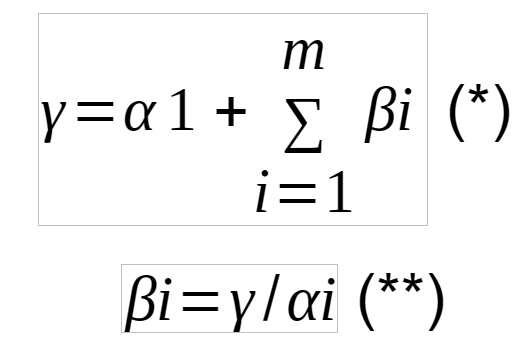
\includegraphics[width=1.57292in,height=\textheight]{imagens/formula.png}

}

\caption{\label{fig-formula}Fórmula da partição aditiva (*\emph{) e
multiplicativa (}**).}

\end{figure}%

Na \textbf{partição aditiva (*)} (Oksanen et al., 2020), γ é expressa
como a soma da diversidade alfa do nível amostral (α₁) e das
contribuições da diversidade beta (βᵢ) associadas a cada unidade
amostral, conforme a equação γ = α₁ + Σβᵢ Figure~\ref{fig-formula}. A
diversidade (βᵢ) foi calculada a partir da razão entre a diversidade
total (γ) e a diversidade alfa observada em cada unidade amostral (αᵢ),
permitindo avaliar o grau de diferenciação entre as unidades amostrais
em relação ao conjunto total de amostras. Valores mais elevados de βᵢ
indicam maior heterogeneidade entre as unidades amostrais, enquanto
valores menores sugerem maior similaridade entre elas. Em resumo, a
diversidade total (\textbf{γ}) é resultado da diversidade média local
(\textbf{α₁}) e da soma das diferenças entre as unidades amostrais
(\textbf{βᵢ}). A \textbf{partição multiplicativa (**)} tem como função
encontrar o valor da diversidade beta (β), tendo em vista que a
diversidade de espécies muda ao longo de escalas espaciais (Jost, 2007;
Lande, 1996; Melo et al., 2009; Melo et al., 2012; Whittaker, 1972;
\textbf{oksanen2025?}).

\subsection{Statistical Analyses}\label{statistical-analyses}

Os dados foram organizados em formatos de tabelas, gráficos e figuras e
analisados por meio de testes estatísticos compatíveis através de
técnicas multivariadas utilizando o ambiente de programação R/RStudio
(Hair et al., 2021; R Core Team, 2017; RStudio Team, 2022; Zar, 1999).

Para a realização das análises estatísticas, foram utilizados pacotes
que permitem avaliar a estrutura da comunidade com base na riqueza. A
Análise de Componentes Principais (PCA) foi executada para avaliar as
variáveis ambientais.

Foram empregados pacotes sobre partição da diversidade para que fosse
possível decompor ou particionar a diversidade em componentes alfa (α),
beta (β) e gama (γ). A diversidade alfa se refere à diversidade de
espécies em uma escala local, ou seja, dentro de manchas homogêneas
locais ou unidades amostrais únicas. Diversidade gama, ou diversidade
regional, corresponde a escalas espaciais maiores, enquanto que a
diversidade beta manifesta-se quando há variação na diversidade entre os
ambientes ou escalas espaciais (Chao et al., 2012; Farias et al., 2020).

Os gráficos e figuras sobre as partições foram realizados no programa
estatístico RStudio utilizando os pacotes: eulerr, vegan e VennDiagram
que forneceram informações acerca da distribuição da riqueza de espécies
com base na diversidade alfa e diversidade gama (Chen \& Boutros, 2011;
\textbf{oksanen2015?}). Funções como adipart e multipart também foram
empregadas. A função adipart foi utilizada para a partição aditiva da
diversidade, em que conterá os valores médios da diversidade alfa que
serão comparados com a diversidade total em todo o conjunto de dados
(γ-diversidade) e multipart para partição multiplicativa da diversidade,
que conterá os valores médios da α-diversidade em níveis mais baixos de
uma hierarquia e comparados com a diversidade total gama.

Esses pacotes permitiram uma análise detalhada e abrangente da
distribuição e diversidade de espécies nos riachos estudados.

\begin{Shaded}
\begin{Highlighting}[numbers=left,,]
\CommentTok{\#REBIO23 {-} ORGANIZANDO DADOS{-}{-}{-}{-}}
\DocumentationTok{\#\#\#\#\#....{-}{-}{-}{-}}

\FunctionTok{dev.off}\NormalTok{() }\CommentTok{\#apaga os graficos, se houver algum}
\FunctionTok{rm}\NormalTok{(}\AttributeTok{list=}\FunctionTok{ls}\NormalTok{(}\AttributeTok{all=}\ConstantTok{TRUE}\NormalTok{)) }\CommentTok{\#limpa a memória}
\FunctionTok{cat}\NormalTok{(}\StringTok{"}\SpecialCharTok{\textbackslash{}014}\StringTok{"}\NormalTok{) }\CommentTok{\#limpa o console}
\CommentTok{\#shell.exec(getwd())}
\FunctionTok{getwd}\NormalTok{()}
\FunctionTok{setwd}\NormalTok{(}\StringTok{"C:/Users/ellen/Downloads"}\NormalTok{)}
\FunctionTok{library}\NormalTok{(openxlsx)}

\DocumentationTok{\#\#CARREGANDO MATRIZES BRUTAS{-}{-}{-}{-}}

\NormalTok{habitat }\OtherTok{\textless{}{-}} \FunctionTok{read.xlsx}\NormalTok{(}\StringTok{"C:/Users/ellen/Dropbox/Universidade/Estágio/Planilhas REBIO23/rebio23{-}habitat.xlsx"}\NormalTok{,}
                    \AttributeTok{rowNames =}\NormalTok{ T,}
                    \AttributeTok{colNames =}\NormalTok{ T,}
                    \AttributeTok{sheet =} \StringTok{"ambiente"}\NormalTok{)}
\NormalTok{grupos }\OtherTok{\textless{}{-}} \FunctionTok{read.xlsx}\NormalTok{(}\StringTok{"C:/Users/ellen/Dropbox/Universidade/Estágio/Planilhas REBIO23/rebio23{-}habitat.xlsx"}\NormalTok{,}
                   \AttributeTok{rowNames =}\NormalTok{ T,}
                   \AttributeTok{colNames =}\NormalTok{ T,}
                   \AttributeTok{sheet =} \StringTok{"grupos"}\NormalTok{)}

\DocumentationTok{\#\#\#REMOVENDO LINHAS ZERADAS DE HABITAT{-}{-}{-}{-}}
\FunctionTok{rownames}\NormalTok{(habitat)}
\NormalTok{del\_rows }\OtherTok{\textless{}{-}} \FunctionTok{c}\NormalTok{(}\StringTok{"S{-}C{-}P11{-}H1"}\NormalTok{, }\StringTok{"S{-}C{-}P11{-}H2"}\NormalTok{, }\StringTok{"S{-}C{-}P11{-}H3"}\NormalTok{, }\StringTok{"C{-}C{-}P11{-}H1"}\NormalTok{,}\StringTok{"C{-}C{-}P11{-}H2"}\NormalTok{,}\StringTok{"C{-}C{-}P11{-}H3"}\NormalTok{)}
\NormalTok{del\_rows}
\NormalTok{m\_hab }\OtherTok{\textless{}{-}}\NormalTok{ habitat[}\SpecialCharTok{!}\NormalTok{(}\FunctionTok{row.names}\NormalTok{(habitat) }\SpecialCharTok{\%in\%} \FunctionTok{c}\NormalTok{(del\_rows)),]}
\NormalTok{m\_hab}

\DocumentationTok{\#\#\#REMOVENDO LINHAS ZERADAS DE GRUPOS{-}{-}{-}{-}}
\FunctionTok{rownames}\NormalTok{(grupos)}
\NormalTok{del\_rows }\OtherTok{\textless{}{-}} \FunctionTok{c}\NormalTok{(}\StringTok{"S{-}C{-}P11{-}H1"}\NormalTok{, }\StringTok{"S{-}C{-}P11{-}H2"}\NormalTok{, }\StringTok{"S{-}C{-}P11{-}H3"}\NormalTok{, }\StringTok{"C{-}C{-}P11{-}H1"}\NormalTok{,}\StringTok{"C{-}C{-}P11{-}H2"}\NormalTok{,}\StringTok{"C{-}C{-}P11{-}H3"}\NormalTok{)}
\NormalTok{del\_rows}
\NormalTok{grupos }\OtherTok{\textless{}{-}}\NormalTok{ grupos[}\SpecialCharTok{!}\NormalTok{(}\FunctionTok{row.names}\NormalTok{(grupos) }\SpecialCharTok{\%in\%} \FunctionTok{c}\NormalTok{(del\_rows)),]}
\NormalTok{grupos}

\DocumentationTok{\#\#\#PARTICIONANDO TABELA DE GRUPOS{-}{-}{-}{-}}
\NormalTok{t\_grps }\OtherTok{\textless{}{-}}\NormalTok{ grupos[}\SpecialCharTok{!}\NormalTok{(}\FunctionTok{row.names}\NormalTok{(grupos) }\SpecialCharTok{\%in\%}\NormalTok{ del\_rows),]}


\DocumentationTok{\#\#SALVANDO MATRIZES FINAIS REMOVIDAS AS LINHAS/COLUNAS ZERADAS{-}{-}{-}{-}}

\FunctionTok{write.table}\NormalTok{(t\_grps, }\StringTok{"t\_grps.csv"}\NormalTok{,}
            \AttributeTok{sep =} \StringTok{";"}\NormalTok{, }\AttributeTok{dec =} \StringTok{"."}\NormalTok{, }\CommentTok{\#"\textbackslash{}t",}
            \AttributeTok{row.names =} \ConstantTok{TRUE}\NormalTok{,}
            \AttributeTok{quote =} \ConstantTok{TRUE}\NormalTok{,}
            \AttributeTok{append =} \ConstantTok{FALSE}\NormalTok{)}
\FunctionTok{write.table}\NormalTok{(m\_hab, }\StringTok{"m\_hab.csv"}\NormalTok{,}
            \AttributeTok{sep =} \StringTok{";"}\NormalTok{, }\AttributeTok{dec =} \StringTok{"."}\NormalTok{, }\CommentTok{\#"\textbackslash{}t",}
            \AttributeTok{row.names =} \ConstantTok{TRUE}\NormalTok{,}
            \AttributeTok{quote =} \ConstantTok{TRUE}\NormalTok{,}
            \AttributeTok{append =} \ConstantTok{FALSE}\NormalTok{)}
\NormalTok{t\_grps }\OtherTok{\textless{}{-}} \FunctionTok{read.csv}\NormalTok{(}\StringTok{"t\_grps.csv"}\NormalTok{,}
                   \AttributeTok{sep =} \StringTok{";"}\NormalTok{, }\AttributeTok{dec =} \StringTok{"."}\NormalTok{,}
                   \AttributeTok{row.names =} \DecValTok{1}\NormalTok{,}
                   \AttributeTok{header =} \ConstantTok{TRUE}\NormalTok{,}
                   \AttributeTok{na.strings =} \ConstantTok{NA}\NormalTok{)}
\NormalTok{m\_hab }\OtherTok{\textless{}{-}} \FunctionTok{read.csv}\NormalTok{(}\StringTok{"m\_hab.csv"}\NormalTok{,}
                   \AttributeTok{sep =} \StringTok{";"}\NormalTok{, }\AttributeTok{dec =} \StringTok{"."}\NormalTok{,}
                   \AttributeTok{row.names =} \DecValTok{1}\NormalTok{,}
                   \AttributeTok{header =} \ConstantTok{TRUE}\NormalTok{,}
                   \AttributeTok{na.strings =} \ConstantTok{NA}\NormalTok{)}

\CommentTok{\#REBIO23 {-} MATRIZ DE CONTAGEM{-}{-}{-}{-}}
\DocumentationTok{\#\#\#\#\#....{-}{-}{-}{-}}

\FunctionTok{library}\NormalTok{(openxlsx)}
\NormalTok{zoo }\OtherTok{\textless{}{-}} \FunctionTok{read.xlsx}\NormalTok{(}\StringTok{"C:/Users/ellen/Dropbox/Universidade/Estágio/Planilhas REBIO23/rebio23{-}zoopl.xlsx"}\NormalTok{,}
                       \AttributeTok{rowNames =}\NormalTok{ T,}
                       \AttributeTok{colNames =}\NormalTok{ T,}
                       \AttributeTok{sheet =} \StringTok{"rebio23\_80ml"}\NormalTok{)}
\NormalTok{zoo [}\DecValTok{1}\SpecialCharTok{:}\DecValTok{5}\NormalTok{,}\DecValTok{1}\SpecialCharTok{:}\DecValTok{5}\NormalTok{] }\CommentTok{\#[1:5,1:5] mostra apenas as linhas e colunas de 1 a 5.}

\FunctionTok{str}\NormalTok{(zoo)}
\CommentTok{\#View(zoo)}
\NormalTok{zoo[}\DecValTok{1}\SpecialCharTok{:}\DecValTok{5}\NormalTok{,}\DecValTok{1}\SpecialCharTok{:}\DecValTok{5}\NormalTok{] }\CommentTok{\#[1:5,1:5] mostra apenas as linhas e colunas de 1 a 5.}
\CommentTok{\#View(zoo)}
\FunctionTok{print}\NormalTok{(zoo[}\DecValTok{1}\SpecialCharTok{:}\DecValTok{8}\NormalTok{,}\DecValTok{1}\SpecialCharTok{:}\DecValTok{8}\NormalTok{])}
\FunctionTok{str}\NormalTok{(zoo)}
\FunctionTok{mode}\NormalTok{(zoo)}
\FunctionTok{class}\NormalTok{(zoo)}

\DocumentationTok{\#\#\#REMOVENDO LINHAS ZERADAS}
\FunctionTok{rownames}\NormalTok{(zoo)}
\NormalTok{del\_rows }\OtherTok{\textless{}{-}} \FunctionTok{c}\NormalTok{(}\StringTok{"S{-}C{-}P11{-}H1"}\NormalTok{, }\StringTok{"S{-}C{-}P11{-}H2"}\NormalTok{, }\StringTok{"S{-}C{-}P11{-}H3"}\NormalTok{, }\StringTok{"C{-}C{-}P11{-}H1"}\NormalTok{,}\StringTok{"C{-}C{-}P11{-}H2"}\NormalTok{,}\StringTok{"C{-}C{-}P11{-}H3"}\NormalTok{)}
\NormalTok{del\_rows}
\NormalTok{zoo }\OtherTok{\textless{}{-}}\NormalTok{ zoo[}\SpecialCharTok{!}\NormalTok{(}\FunctionTok{row.names}\NormalTok{(zoo) }\SpecialCharTok{\%in\%} \FunctionTok{c}\NormalTok{(del\_rows)),]}
\NormalTok{zoo}
\FunctionTok{colnames}\NormalTok{(zoo)}
\NormalTok{m\_trab }\OtherTok{\textless{}{-}}\NormalTok{ zoo}
\FunctionTok{colnames}\NormalTok{(m\_trab) }\OtherTok{\textless{}{-}} \FunctionTok{as.character}\NormalTok{(}\FunctionTok{unlist}\NormalTok{(m\_trab[}\DecValTok{1}\NormalTok{, ]))}
\NormalTok{m\_trab }\OtherTok{\textless{}{-}}\NormalTok{ m\_trab[}\SpecialCharTok{{-}}\DecValTok{1}\NormalTok{, ]}

\CommentTok{\#Criando a matriz de cada período}
\NormalTok{zoo\_seco }\OtherTok{\textless{}{-}}\NormalTok{ m\_trab[}\FunctionTok{grepl}\NormalTok{(}\StringTok{"\^{}S"}\NormalTok{, }\FunctionTok{rownames}\NormalTok{(m\_trab)), ]}
\NormalTok{zoo\_chuvoso }\OtherTok{\textless{}{-}}\NormalTok{ m\_trab[}\FunctionTok{grepl}\NormalTok{(}\StringTok{"\^{}C"}\NormalTok{, }\FunctionTok{rownames}\NormalTok{(m\_trab)), ]}

\DocumentationTok{\#\#SALVANDO MATRIZ FINAL}
\CommentTok{\#PERÍODO SECO}
\FunctionTok{write.table}\NormalTok{(zoo\_seco, }\StringTok{"zoo\_seco.csv"}\NormalTok{,}
            \AttributeTok{sep =} \StringTok{";"}\NormalTok{, }\AttributeTok{dec =} \StringTok{"."}\NormalTok{, }\CommentTok{\#"\textbackslash{}t",}
            \AttributeTok{row.names =} \ConstantTok{TRUE}\NormalTok{,}
            \AttributeTok{quote =} \ConstantTok{TRUE}\NormalTok{,}
            \AttributeTok{append =} \ConstantTok{FALSE}\NormalTok{)}
\NormalTok{zoo\_seco }\OtherTok{\textless{}{-}} \FunctionTok{read.csv}\NormalTok{(}\StringTok{"zoo\_seco.csv"}\NormalTok{,}
                   \AttributeTok{sep =} \StringTok{";"}\NormalTok{, }\AttributeTok{dec =} \StringTok{"."}\NormalTok{,}
                   \AttributeTok{row.names =} \DecValTok{1}\NormalTok{,}
                   \AttributeTok{header =} \ConstantTok{TRUE}\NormalTok{,}
                   \AttributeTok{na.strings =} \ConstantTok{NA}\NormalTok{)}
\NormalTok{zoo\_seco}

\CommentTok{\#PERÍODO CHUVOSO}
\FunctionTok{write.table}\NormalTok{(zoo\_chuvoso, }\StringTok{"zoo\_chuvoso.csv"}\NormalTok{,}
            \AttributeTok{sep =} \StringTok{";"}\NormalTok{, }\AttributeTok{dec =} \StringTok{"."}\NormalTok{, }\CommentTok{\#"\textbackslash{}t",}
            \AttributeTok{row.names =} \ConstantTok{TRUE}\NormalTok{,}
            \AttributeTok{quote =} \ConstantTok{TRUE}\NormalTok{,}
            \AttributeTok{append =} \ConstantTok{FALSE}\NormalTok{)}
\NormalTok{zoo\_chuvoso }\OtherTok{\textless{}{-}} \FunctionTok{read.csv}\NormalTok{(}\StringTok{"zoo\_chuvoso.csv"}\NormalTok{,}
                     \AttributeTok{sep =} \StringTok{";"}\NormalTok{, }\AttributeTok{dec =} \StringTok{"."}\NormalTok{,}
                     \AttributeTok{row.names =} \DecValTok{1}\NormalTok{,}
                     \AttributeTok{header =} \ConstantTok{TRUE}\NormalTok{,}
                     \AttributeTok{na.strings =} \ConstantTok{NA}\NormalTok{)}
\NormalTok{zoo\_chuvoso}
\end{Highlighting}
\end{Shaded}

\section{Results}\label{results}

The results section should follow the model in
\url{https://elviomedeiros.github.io/Bentos2006_Q/}.

\subsection{Environmental variables}\label{environmental-variables}

É importante destacar que as unidades amostrais (UAs) P05 a P10
correspondem ao riacho Barro Branco, sendo as UAs P5, P6 e P7
localizadas no interior da reserva, enquanto que os pontos P08, P09 e
P10 estão situados fora da área de preservação. O riacho Caiana, por sua
vez, é representado pelas UAs P12 a P20, todas localizadas fora da
reserva (ver Figure~\ref{fig-mapa}).

Os resultados da Análise de Componentes Principais (PCA) evidenciaram
uma clara diferenciação das unidades amostrais com base nas
características físicas e estruturais do habitat. Ao longo dos riachos e
períodos amostrais analisados.

No período seco (Figure~\ref{fig-pcaseco}), observou-se que as UAs P05,
P07 e P08, pertencentes ao riacho Barro Branco, apresentaram maior
associação a liteira, algas filamentosas e aderidas. Em contraste, a UA
P06 do Barro Branco, juntamente com as UAs P16, P17 e P20, do Caiana,
esteve associada principalmente às variáveis estruturais, como a
presença de pedras, profundidade máxima, mínima e marginal, largura e
vegetação submersa. Além disso, P10 do Barro Branco e P18 do Caiana
apresentaram associação evidente ao pH, cujos valores variaram de ácido
a levemente neutro.

No período chuvoso (Figure~\ref{fig-pcachuvoso}), a distribuição das
unidades amostrais no espaço da biplot indicou alterações nos padrões de
associação observados no período seco. As UAs P05 e P06 do Barro Branco,
assim como a UA P18 do Caiana, estiveram associadas principalmente à
presença de lama, macrófitas, vegetação submersa, folhiço e detritos.
Por outro lado, as P08, P10 e P16 apresentaram maior associação com
algas filamentosas e aderidas, vegetação marginal e largura média do
canal.

De modo geral, os resultados indicaram que ambos os períodos
contribuíram de formas distintas para a estruturação do habitat,
evidenciando variações espaciais e sazonais nas características físicas
e estruturais dos riachos estudados.

\begin{Shaded}
\begin{Highlighting}[numbers=left,,]
\CommentTok{\#REBIO23 {-} PCA {-} SECO{-}{-}{-}{-}}
\DocumentationTok{\#\#\#\#\#....{-}{-}{-}{-}}

\FunctionTok{dev.off}\NormalTok{()}
\FunctionTok{rm}\NormalTok{(}\AttributeTok{list=}\FunctionTok{ls}\NormalTok{(}\AttributeTok{all=}\ConstantTok{TRUE}\NormalTok{))}
\FunctionTok{cat}\NormalTok{(}\StringTok{"}\SpecialCharTok{\textbackslash{}014}\StringTok{"}\NormalTok{)}
\FunctionTok{library}\NormalTok{(openxlsx)}
\NormalTok{dados\_bruto }\OtherTok{\textless{}{-}} \FunctionTok{read.xlsx}\NormalTok{(}\StringTok{"C:/Users/ellen/Dropbox/Universidade/Estágio/Planilhas REBIO23/rebio{-}habitat.xlsx"}\NormalTok{,}
                         \AttributeTok{rowNames =}\NormalTok{ T,}
                         \AttributeTok{colNames =}\NormalTok{ T,}
                         \AttributeTok{sheet =} \StringTok{"habitat\_t"}\NormalTok{,}
                         \AttributeTok{na.strings =} \StringTok{"n/a"}\NormalTok{,}
                         \AttributeTok{startRow =} \DecValTok{2}\NormalTok{)}

\CommentTok{\#deletar o ponto onze}
\FunctionTok{row.names}\NormalTok{(dados\_bruto)}
\NormalTok{del\_rows }\OtherTok{\textless{}{-}} \FunctionTok{c}\NormalTok{(}\StringTok{"S{-}C{-}P11{-}H1"}\NormalTok{, }\StringTok{"S{-}C{-}P11{-}H2"}\NormalTok{, }\StringTok{"S{-}C{-}P11{-}H3"}\NormalTok{, }\StringTok{"C{-}C{-}P11{-}H1"}\NormalTok{, }\StringTok{"C{-}C{-}P11{-}H2"}\NormalTok{, }\StringTok{"C{-}C{-}P11{-}H3"}\NormalTok{)}
\NormalTok{m\_cort }\OtherTok{\textless{}{-}}\NormalTok{ dados\_bruto[}\SpecialCharTok{!}\NormalTok{(}\FunctionTok{row.names}\NormalTok{(dados\_bruto) }\SpecialCharTok{\%in\%}\NormalTok{ del\_rows), ]}

\CommentTok{\#SELECIONANDO VARIÁVEIS}
\NormalTok{m\_cort }\OtherTok{\textless{}{-}}\NormalTok{ m\_cort [, }\FunctionTok{c}\NormalTok{(}\StringTok{"Cond\_uS.cm"}\NormalTok{,}\StringTok{"Turb\_ntu"}\NormalTok{, }\StringTok{"pH"}\NormalTok{, }\StringTok{"Vel\_m.s"}\NormalTok{, }\StringTok{"Slope"}\NormalTok{, }\StringTok{"Depth\_max\_cm"}\NormalTok{,}
                      \StringTok{"Depth\_avg\_cm"}\NormalTok{, }\StringTok{"Depth\_mar\_cm"}\NormalTok{, }\StringTok{"Width\_m"}\NormalTok{, }\StringTok{"Mud"}\NormalTok{, }\StringTok{"Sand"}\NormalTok{, }\StringTok{"Gravel\_f"}\NormalTok{, }
                      \StringTok{"Gravel\_c"}\NormalTok{, }\StringTok{"Cobbles"}\NormalTok{, }\StringTok{"Rocks"}\NormalTok{, }\StringTok{"Bedrock"}\NormalTok{, }\StringTok{"Macrophytes"}\NormalTok{, }\StringTok{"Grass"}\NormalTok{, }
                      \StringTok{"Subm\_veg"}\NormalTok{, }\StringTok{"Overh\_veg"}\NormalTok{, }\StringTok{"Leaf\_l"}\NormalTok{, }\StringTok{"Algae\_f"}\NormalTok{, }\StringTok{"Algae\_a"}\NormalTok{, }\StringTok{"Root\_masses"}\NormalTok{,}
                      \StringTok{"Debris\_l"}\NormalTok{, }\StringTok{"Debris\_s"}\NormalTok{)]}
\FunctionTok{str}\NormalTok{(m\_cort)}

\CommentTok{\# CRIANDO MATRIZ DE MÉDIAS}
\FunctionTok{library}\NormalTok{(}\StringTok{"tidyverse"}\NormalTok{)}
\CommentTok{\#Inserindo coluna para agrupamentos}
\NormalTok{data }\OtherTok{\textless{}{-}}\NormalTok{ m\_cort}
\FunctionTok{nrow}\NormalTok{(data); }\FunctionTok{ncol}\NormalTok{(data) }\CommentTok{\#no. de N colunas x M linhas}
\NormalTok{data\_g }\OtherTok{\textless{}{-}} \FunctionTok{cbind}\NormalTok{(}\AttributeTok{Grupos =} \FunctionTok{rownames}\NormalTok{(data), data)}
\NormalTok{data\_g}
\NormalTok{grps }\OtherTok{\textless{}{-}} \FunctionTok{substr}\NormalTok{(data\_g[, }\DecValTok{1}\NormalTok{], }\DecValTok{1}\NormalTok{,}\DecValTok{7}\NormalTok{)}
\NormalTok{grps}
\NormalTok{data\_g }\OtherTok{\textless{}{-}}\NormalTok{ data\_g }\SpecialCharTok{\%\textgreater{}\%} \FunctionTok{mutate}\NormalTok{(}\AttributeTok{Grupos=}\FunctionTok{c}\NormalTok{(grps))}
\CommentTok{\#data\_avg \textless{}{-} aggregate(data\_g[, 9:9], list(data\_g$Grupos), mean)}
\CommentTok{\#data\_avg}
\NormalTok{data\_avg }\OtherTok{\textless{}{-}}\NormalTok{ data\_g }\SpecialCharTok{\%\textgreater{}\%} 
  \FunctionTok{group\_by}\NormalTok{(Grupos) }\SpecialCharTok{\%\textgreater{}\%}
  \FunctionTok{summarise}\NormalTok{(}\FunctionTok{across}\NormalTok{(}\AttributeTok{.cols =} \FunctionTok{everything}\NormalTok{(), }\SpecialCharTok{\textasciitilde{}} \FunctionTok{mean}\NormalTok{(.x, }\AttributeTok{na.rm =} \ConstantTok{TRUE}\NormalTok{)))}
\NormalTok{data\_avg}
\NormalTok{data\_dp }\OtherTok{\textless{}{-}}\NormalTok{ data\_g }\SpecialCharTok{\%\textgreater{}\%} 
  \FunctionTok{group\_by}\NormalTok{(Grupos) }\SpecialCharTok{\%\textgreater{}\%}
  \FunctionTok{summarise}\NormalTok{(}\FunctionTok{across}\NormalTok{(}\AttributeTok{.cols =} \FunctionTok{everything}\NormalTok{(), }\FunctionTok{list}\NormalTok{(}\AttributeTok{mean =}\NormalTok{ mean, }\AttributeTok{sd =}\NormalTok{ sd)))}
\CommentTok{\#?across}
\NormalTok{data\_dp }\OtherTok{\textless{}{-}}\NormalTok{ data\_avg}
\CommentTok{\#Primeira coluna para nomes das linhas }
\NormalTok{data\_dp }\OtherTok{\textless{}{-}} \FunctionTok{as.data.frame}\NormalTok{(data\_dp)}
\FunctionTok{class}\NormalTok{(data\_dp)}
\FunctionTok{rownames}\NormalTok{(data\_dp) }\OtherTok{\textless{}{-}}\NormalTok{ data\_dp[,}\DecValTok{1}\NormalTok{]}
\NormalTok{data\_dp[,}\DecValTok{1}\NormalTok{] }\OtherTok{\textless{}{-}} \ConstantTok{NULL}
\NormalTok{data\_dp }\OtherTok{\textless{}{-}} \FunctionTok{round}\NormalTok{(data\_dp, }\DecValTok{1}\NormalTok{)}
\NormalTok{data\_dp}
\NormalTok{m\_cort }\OtherTok{\textless{}{-}}\NormalTok{ data\_dp}

\CommentTok{\#SELECIONANDO VARIÁVEIS}
\NormalTok{m\_trans }\OtherTok{\textless{}{-}} \FunctionTok{t}\NormalTok{(m\_cort)}
\FunctionTok{colnames}\NormalTok{(m\_trans)}
\NormalTok{seco }\OtherTok{\textless{}{-}} \FunctionTok{t}\NormalTok{(m\_trans[, }\FunctionTok{c}\NormalTok{(}\StringTok{"S{-}B{-}P05"}\NormalTok{, }\StringTok{"S{-}B{-}P06"}\NormalTok{, }\StringTok{"S{-}B{-}P07"}\NormalTok{,}
                      \StringTok{"S{-}B{-}P08"}\NormalTok{, }\StringTok{"S{-}B{-}P09"}\NormalTok{, }\StringTok{"S{-}B{-}P10"}\NormalTok{, }
                      \StringTok{"S{-}C{-}P12"}\NormalTok{, }\StringTok{"S{-}C{-}P13"}\NormalTok{, }\StringTok{"S{-}C{-}P14"}\NormalTok{,}
                      \StringTok{"S{-}C{-}P15"}\NormalTok{, }\StringTok{"S{-}C{-}P16"}\NormalTok{, }\StringTok{"S{-}C{-}P17"}\NormalTok{,}
                      \StringTok{"S{-}C{-}P18"}\NormalTok{, }\StringTok{"S{-}C{-}P19"}\NormalTok{, }\StringTok{"S{-}C{-}P20"}\NormalTok{)])}

\NormalTok{chuvoso }\OtherTok{\textless{}{-}} \FunctionTok{t}\NormalTok{(m\_trans[, }\FunctionTok{c}\NormalTok{(}\StringTok{"C{-}B{-}P05"}\NormalTok{, }\StringTok{"C{-}B{-}P06"}\NormalTok{, }\StringTok{"C{-}B{-}P07"}\NormalTok{, }
                         \StringTok{"C{-}B{-}P08"}\NormalTok{, }\StringTok{"C{-}B{-}P09"}\NormalTok{, }\StringTok{"C{-}B{-}P10"}\NormalTok{,}
                         \StringTok{"C{-}C{-}P12"}\NormalTok{, }\StringTok{"C{-}C{-}P13"}\NormalTok{, }\StringTok{"C{-}C{-}P14"}\NormalTok{,}
                         \StringTok{"C{-}C{-}P15"}\NormalTok{, }\StringTok{"C{-}C{-}P16"}\NormalTok{, }\StringTok{"C{-}C{-}P17"}\NormalTok{,}
                         \StringTok{"C{-}C{-}P18"}\NormalTok{, }\StringTok{"C{-}C{-}P19"}\NormalTok{, }\StringTok{"C{-}C{-}P20"}\NormalTok{)])}

\DocumentationTok{\#\#\#\#\#\# seco}
\NormalTok{seco }\OtherTok{\textless{}{-}} \FunctionTok{as.data.frame}\NormalTok{(seco)}
\NormalTok{seco[] }\OtherTok{\textless{}{-}} \FunctionTok{lapply}\NormalTok{(seco, as.numeric)}
\DocumentationTok{\#\#\#\#\#\# chuvoso}
\NormalTok{chuvoso }\OtherTok{\textless{}{-}} \FunctionTok{as.data.frame}\NormalTok{(chuvoso)}
\NormalTok{chuvoso[] }\OtherTok{\textless{}{-}} \FunctionTok{lapply}\NormalTok{(chuvoso, as.numeric)}

\DocumentationTok{\#\#\#\#\#\#\#\#\#\#\#\#\#\#\#\#\#\#\#\#\#\#\#\#\#\#\#\#\#\#\#\#\#\#\#\#\#\#\#\#\#\#\#\#\#\#\#\#\#\#\#\#\#\#\#\#\#\#\#\#\#\#\#\#\#\#\#\#\#\#\#\#\#\#\#\#\#\#\#\#}
\DocumentationTok{\#\#\#\#SECO}

\CommentTok{\# CRIANDO MATRIZ DE MÉDIAS}
\FunctionTok{library}\NormalTok{(}\StringTok{"tidyverse"}\NormalTok{)}
\CommentTok{\#Inserindo coluna para agrupamentos}
\NormalTok{data }\OtherTok{\textless{}{-}}\NormalTok{ seco}
\FunctionTok{nrow}\NormalTok{(data); }\FunctionTok{ncol}\NormalTok{(data) }\CommentTok{\#no. de N colunas x M linhas}
\NormalTok{data\_g }\OtherTok{\textless{}{-}} \FunctionTok{cbind}\NormalTok{(}\AttributeTok{Grupos =} \FunctionTok{rownames}\NormalTok{(data), data)}
\NormalTok{data\_g}
\NormalTok{grps }\OtherTok{\textless{}{-}} \FunctionTok{substr}\NormalTok{(data\_g[, }\DecValTok{1}\NormalTok{], }\DecValTok{5}\NormalTok{,}\DecValTok{7}\NormalTok{)}
\NormalTok{grps}
\NormalTok{data\_g }\OtherTok{\textless{}{-}}\NormalTok{ data\_g }\SpecialCharTok{\%\textgreater{}\%} \FunctionTok{mutate}\NormalTok{(}\AttributeTok{Grupos=}\FunctionTok{c}\NormalTok{(grps))}
\CommentTok{\#data\_avg \textless{}{-} aggregate(data\_g[, 9:9], list(data\_g$Grupos), mean)}
\CommentTok{\#data\_avg}
\NormalTok{data\_avg }\OtherTok{\textless{}{-}}\NormalTok{ data\_g }\SpecialCharTok{\%\textgreater{}\%} 
  \FunctionTok{group\_by}\NormalTok{(Grupos) }\SpecialCharTok{\%\textgreater{}\%}
  \FunctionTok{summarise}\NormalTok{(}\FunctionTok{across}\NormalTok{(}\AttributeTok{.cols =} \FunctionTok{everything}\NormalTok{(), }\SpecialCharTok{\textasciitilde{}} \FunctionTok{mean}\NormalTok{(.x, }\AttributeTok{na.rm =} \ConstantTok{TRUE}\NormalTok{)))}
\NormalTok{data\_avg}
\NormalTok{data\_dp }\OtherTok{\textless{}{-}}\NormalTok{ data\_g }\SpecialCharTok{\%\textgreater{}\%} 
  \FunctionTok{group\_by}\NormalTok{(Grupos) }\SpecialCharTok{\%\textgreater{}\%}
  \FunctionTok{summarise}\NormalTok{(}\FunctionTok{across}\NormalTok{(}\AttributeTok{.cols =} \FunctionTok{everything}\NormalTok{(), }\FunctionTok{list}\NormalTok{(}\AttributeTok{mean =}\NormalTok{ mean, }\AttributeTok{sd =}\NormalTok{ sd)))}
\CommentTok{\#?across}
\NormalTok{data\_dp }\OtherTok{\textless{}{-}}\NormalTok{ data\_avg}
\CommentTok{\#Primeira coluna para nomes das linhas }
\NormalTok{data\_dp }\OtherTok{\textless{}{-}} \FunctionTok{as.data.frame}\NormalTok{(data\_dp)}
\FunctionTok{class}\NormalTok{(data\_dp)}
\FunctionTok{rownames}\NormalTok{(data\_dp) }\OtherTok{\textless{}{-}}\NormalTok{ data\_dp[,}\DecValTok{1}\NormalTok{]}
\NormalTok{data\_dp[,}\DecValTok{1}\NormalTok{] }\OtherTok{\textless{}{-}} \ConstantTok{NULL}
\NormalTok{data\_dp }\OtherTok{\textless{}{-}} \FunctionTok{round}\NormalTok{(data\_dp, }\DecValTok{1}\NormalTok{)}
\NormalTok{data\_dp}
\NormalTok{seco }\OtherTok{\textless{}{-}}\NormalTok{ data\_dp}
\DocumentationTok{\#\#\#\#\#\#\#\#\#\#\#\#\#\#\#\#\#\#\#\#\#\#\#\#\#\#\#\#}
\CommentTok{\# Pacotes}
\DocumentationTok{\#\#\#\#\#\#\#\#\#\#\#\#\#\#\#\#\#\#\#\#\#\#\#\#\#\#\#\#}
\FunctionTok{library}\NormalTok{(vegan)}
\FunctionTok{library}\NormalTok{(gplots)}
\FunctionTok{library}\NormalTok{(psych)}
\FunctionTok{library}\NormalTok{(tidyverse)}
\FunctionTok{library}\NormalTok{(ggplot2)}

\DocumentationTok{\#\#\#\#\#\#\#\#\#\#\#\#\#\#\#\#\#\#\#\#\#\#\#\#\#\#\#\#}
\CommentTok{\# Pré{-}processamento da matriz}
\DocumentationTok{\#\#\#\#\#\#\#\#\#\#\#\#\#\#\#\#\#\#\#\#\#\#\#\#\#\#\#\#}
\NormalTok{m\_trab }\OtherTok{\textless{}{-}}\NormalTok{ seco}
\NormalTok{m\_trns }\OtherTok{\textless{}{-}} \FunctionTok{sqrt}\NormalTok{(m\_trab) }\CommentTok{\# transformação}

\CommentTok{\# Remover linhas e colunas com todos os valores = 0}
\NormalTok{m\_trns }\OtherTok{\textless{}{-}}\NormalTok{ m\_trns[}\FunctionTok{rowSums}\NormalTok{(m\_trns) }\SpecialCharTok{\textgreater{}} \DecValTok{0}\NormalTok{, ]}
\NormalTok{m\_trns }\OtherTok{\textless{}{-}}\NormalTok{ m\_trns[, }\FunctionTok{colSums}\NormalTok{(m\_trns) }\SpecialCharTok{\textgreater{}} \DecValTok{0}\NormalTok{]}

\DocumentationTok{\#\#\#\#\#\#\#\#\#\#\#\#\#\#\#\#\#\#\#\#\#\#\#\#\#\#\#\#}
\CommentTok{\# Distância e Cluster}
\DocumentationTok{\#\#\#\#\#\#\#\#\#\#\#\#\#\#\#\#\#\#\#\#\#\#\#\#\#\#\#\#}
\NormalTok{vegdist\_mat }\OtherTok{\textless{}{-}} \FunctionTok{vegdist}\NormalTok{(m\_trns, }\AttributeTok{method =} \StringTok{"bray"}\NormalTok{, }\AttributeTok{diag =} \ConstantTok{TRUE}\NormalTok{, }\AttributeTok{upper =} \ConstantTok{FALSE}\NormalTok{)}
\NormalTok{cluster\_uas }\OtherTok{\textless{}{-}} \FunctionTok{hclust}\NormalTok{(vegdist\_mat, }\AttributeTok{method =} \StringTok{"average"}\NormalTok{)}

\FunctionTok{plot}\NormalTok{(cluster\_uas, }\AttributeTok{main =} \StringTok{"Cluster Dendrogram {-} Bray{-}Curtis"}\NormalTok{, }\AttributeTok{hang =} \FloatTok{0.1}\NormalTok{)}
\FunctionTok{rect.hclust}\NormalTok{(cluster\_uas, }\AttributeTok{k =} \DecValTok{2}\NormalTok{, }\AttributeTok{h =} \ConstantTok{NULL}\NormalTok{)}

\FunctionTok{as.matrix}\NormalTok{(vegdist\_mat)[}\DecValTok{1}\SpecialCharTok{:}\DecValTok{6}\NormalTok{, }\DecValTok{1}\SpecialCharTok{:}\DecValTok{6}\NormalTok{]}

\DocumentationTok{\#\#\#\#\#\#\#\#\#\#\#\#\#\#\#\#\#\#\#\#\#\#\#\#\#\#\#\#}
\CommentTok{\# Heatmap (UAs)}
\DocumentationTok{\#\#\#\#\#\#\#\#\#\#\#\#\#\#\#\#\#\#\#\#\#\#\#\#\#\#\#\#}
\NormalTok{col }\OtherTok{\textless{}{-}} \FunctionTok{rev}\NormalTok{(}\FunctionTok{heat.colors}\NormalTok{(}\DecValTok{999}\NormalTok{))}

\FunctionTok{heatmap.2}\NormalTok{(}\FunctionTok{as.matrix}\NormalTok{(vegdist\_mat),}
          \AttributeTok{Rowv =} \FunctionTok{as.dendrogram}\NormalTok{(cluster\_uas),}
          \AttributeTok{Colv =} \FunctionTok{as.dendrogram}\NormalTok{(cluster\_uas),}
          \AttributeTok{key =} \ConstantTok{TRUE}\NormalTok{, }\AttributeTok{tracecol =} \ConstantTok{NA}\NormalTok{, }\AttributeTok{revC =} \ConstantTok{TRUE}\NormalTok{,}
          \AttributeTok{col =}\NormalTok{ col,}
          \AttributeTok{density.info =} \StringTok{"none"}\NormalTok{,}
          \AttributeTok{xlab =} \StringTok{"UA´s"}\NormalTok{, }\AttributeTok{ylab =} \StringTok{"UA´s"}\NormalTok{,}
          \AttributeTok{mar =} \FunctionTok{c}\NormalTok{(}\DecValTok{6}\NormalTok{, }\DecValTok{6}\NormalTok{) }\SpecialCharTok{+} \FloatTok{0.2}\NormalTok{)}

\DocumentationTok{\#\#\#\#\#\#\#\#\#\#\#\#\#\#\#\#\#\#\#\#\#\#\#\#\#\#\#\#}
\CommentTok{\# Cluster das variaves}
\DocumentationTok{\#\#\#\#\#\#\#\#\#\#\#\#\#\#\#\#\#\#\#\#\#\#\#\#\#\#\#\#}
\NormalTok{cluster\_spp }\OtherTok{\textless{}{-}} \FunctionTok{hclust}\NormalTok{(}\FunctionTok{vegdist}\NormalTok{(}\FunctionTok{t}\NormalTok{(m\_trns), }\AttributeTok{method =} \StringTok{"bray"}\NormalTok{, }\AttributeTok{diag =} \ConstantTok{TRUE}\NormalTok{, }\AttributeTok{upper =} \ConstantTok{FALSE}\NormalTok{),}
                      \AttributeTok{method =} \StringTok{"average"}\NormalTok{)}
\FunctionTok{plot}\NormalTok{(cluster\_spp, }\AttributeTok{main =} \StringTok{"Dendrograma dos atributos"}\NormalTok{)}

\FunctionTok{heatmap.2}\NormalTok{(}\FunctionTok{t}\NormalTok{(}\FunctionTok{as.matrix}\NormalTok{(m\_trns)),}
          \AttributeTok{Colv =} \FunctionTok{as.dendrogram}\NormalTok{(cluster\_uas),}
          \AttributeTok{Rowv =} \FunctionTok{as.dendrogram}\NormalTok{(cluster\_spp),}
          \AttributeTok{key =} \ConstantTok{TRUE}\NormalTok{, }\AttributeTok{tracecol =} \ConstantTok{NA}\NormalTok{, }\AttributeTok{revC =} \ConstantTok{TRUE}\NormalTok{,}
          \AttributeTok{col =}\NormalTok{ col,}
          \AttributeTok{density.info =} \StringTok{"none"}\NormalTok{,}
          \AttributeTok{xlab =} \StringTok{"Unidades amostrais"}\NormalTok{, }\AttributeTok{ylab =} \StringTok{"Espécies"}\NormalTok{,}
          \AttributeTok{mar =} \FunctionTok{c}\NormalTok{(}\DecValTok{6}\NormalTok{, }\DecValTok{6}\NormalTok{) }\SpecialCharTok{+} \FloatTok{0.1}\NormalTok{)}

\DocumentationTok{\#\#\#\#\#\#\#\#\#\#\#\#\#\#\#\#\#\#\#\#\#\#\#\#\#\#\#\#}
\CommentTok{\# PCA}
\DocumentationTok{\#\#\#\#\#\#\#\#\#\#\#\#\#\#\#\#\#\#\#\#\#\#\#\#\#\#\#\#}
\NormalTok{pca }\OtherTok{\textless{}{-}} \FunctionTok{prcomp}\NormalTok{(m\_trns)}
\FunctionTok{plot}\NormalTok{(pca, }\AttributeTok{type =} \StringTok{"l"}\NormalTok{)}
\FunctionTok{summary}\NormalTok{(pca)}

\FunctionTok{pairs.panels}\NormalTok{(m\_trns[,}\DecValTok{1}\SpecialCharTok{:}\FunctionTok{min}\NormalTok{(}\DecValTok{26}\NormalTok{, }\FunctionTok{ncol}\NormalTok{(m\_trns))], }
             \AttributeTok{method =} \StringTok{"pearson"}\NormalTok{,}
             \AttributeTok{scale =} \ConstantTok{FALSE}\NormalTok{, }\AttributeTok{lm =} \ConstantTok{FALSE}\NormalTok{,}
             \AttributeTok{hist.col =} \StringTok{"\#00AFBB"}\NormalTok{, }\AttributeTok{pch =} \DecValTok{19}\NormalTok{,}
             \AttributeTok{density =} \ConstantTok{TRUE}\NormalTok{, }\AttributeTok{ellipses =} \ConstantTok{TRUE}\NormalTok{, }\AttributeTok{alpha =} \FloatTok{0.5}\NormalTok{)}

\DocumentationTok{\#\#\#\#\#\#\#\#\#\#\#\#\#\#\#\#\#\#\#\#\#\#\#\#\#\#\#\#}
\CommentTok{\# PCA {-} diferentes escalas}
\DocumentationTok{\#\#\#\#\#\#\#\#\#\#\#\#\#\#\#\#\#\#\#\#\#\#\#\#\#\#\#\#}
\NormalTok{pca\_ce }\OtherTok{\textless{}{-}} \FunctionTok{prcomp}\NormalTok{(m\_trns, }\AttributeTok{center =} \ConstantTok{TRUE}\NormalTok{, }\AttributeTok{scale =} \ConstantTok{FALSE}\NormalTok{)}
\NormalTok{pca\_cs }\OtherTok{\textless{}{-}} \FunctionTok{prcomp}\NormalTok{(m\_trns, }\AttributeTok{center =} \ConstantTok{TRUE}\NormalTok{, }\AttributeTok{scale =} \ConstantTok{TRUE}\NormalTok{)}
\NormalTok{pca\_sc }\OtherTok{\textless{}{-}} \FunctionTok{prcomp}\NormalTok{(m\_trns, }\AttributeTok{scale =} \ConstantTok{TRUE}\NormalTok{)}

\FunctionTok{par}\NormalTok{(}\AttributeTok{mfrow =} \FunctionTok{c}\NormalTok{(}\DecValTok{3}\NormalTok{,}\DecValTok{1}\NormalTok{))}
\FunctionTok{plot}\NormalTok{(pca\_ce, }\AttributeTok{type =} \StringTok{"l"}\NormalTok{)}
\FunctionTok{plot}\NormalTok{(pca\_cs, }\AttributeTok{type =} \StringTok{"l"}\NormalTok{)}
\FunctionTok{plot}\NormalTok{(pca\_sc, }\AttributeTok{type =} \StringTok{"l"}\NormalTok{)}
\FunctionTok{par}\NormalTok{(}\AttributeTok{mfrow =} \FunctionTok{c}\NormalTok{(}\DecValTok{1}\NormalTok{,}\DecValTok{1}\NormalTok{))}

\FunctionTok{summary}\NormalTok{(pca\_sc)}
\FunctionTok{plot}\NormalTok{(pca\_sc, }\AttributeTok{type =} \StringTok{"l"}\NormalTok{, }\AttributeTok{main =} \StringTok{"Scree Plot (scaled data {-} m\_trns)"}\NormalTok{)}

\DocumentationTok{\#\#\#\#\#\#\#\#\#\#\#\#\#\#\#\#\#\#\#\#\#\#\#\#\#\#\#\#}
\CommentTok{\# Agrupamentos}
\DocumentationTok{\#\#\#\#\#\#\#\#\#\#\#\#\#\#\#\#\#\#\#\#\#\#\#\#\#\#\#\#}
\NormalTok{add.col }\OtherTok{\textless{}{-}} \FunctionTok{rownames\_to\_column}\NormalTok{(}\FunctionTok{as.data.frame}\NormalTok{(m\_trns), }\AttributeTok{var =} \StringTok{"UAs"}\NormalTok{)}
\NormalTok{agrup }\OtherTok{\textless{}{-}} \FunctionTok{substr}\NormalTok{(add.col}\SpecialCharTok{$}\NormalTok{UAs, }\DecValTok{1}\NormalTok{, }\DecValTok{1}\NormalTok{)}
\NormalTok{m\_pca\_agrup }\OtherTok{\textless{}{-}}\NormalTok{ add.col }\SpecialCharTok{\%\textgreater{}\%}
  \FunctionTok{mutate}\NormalTok{(}\AttributeTok{Agrupamentos =}\NormalTok{ agrup, }\AttributeTok{.before =}\NormalTok{ UAs)}

\DocumentationTok{\#\#\#\#\#\#\#\#\#\#\#\#\#\#\#\#\#\#\#\#\#\#\#\#\#\#\#\#}
\CommentTok{\# Biplot da PCA}
\DocumentationTok{\#\#\#\#\#\#\#\#\#\#\#\#\#\#\#\#\#\#\#\#\#\#\#\#\#\#\#\#}
\NormalTok{pca\_seco }\OtherTok{\textless{}{-}} \FunctionTok{biplot}\NormalTok{(pca\_sc, }\AttributeTok{choices =} \DecValTok{1}\SpecialCharTok{:}\DecValTok{2}\NormalTok{, }\AttributeTok{scale =} \DecValTok{1}\NormalTok{,}
                      \AttributeTok{main =} \StringTok{"Biplot da PCA {-} seco"}\NormalTok{,}
                      \AttributeTok{xlab =} \StringTok{"PC1 UAs"}\NormalTok{, }\AttributeTok{ylab =} \StringTok{"PC2 UAs"}\NormalTok{, }\AttributeTok{cex =} \FloatTok{0.8}\NormalTok{)}
\FunctionTok{ggsave}\NormalTok{(pca\_seco, }\AttributeTok{dpi =} \DecValTok{500}\NormalTok{, }\AttributeTok{filename =} \StringTok{"pca\_seco.png"}\NormalTok{)}

\NormalTok{var\_exp }\OtherTok{\textless{}{-}} \FunctionTok{round}\NormalTok{((pca\_sc}\SpecialCharTok{$}\NormalTok{sdev}\SpecialCharTok{\^{}}\DecValTok{2} \SpecialCharTok{/} \FunctionTok{sum}\NormalTok{(pca\_sc}\SpecialCharTok{$}\NormalTok{sdev}\SpecialCharTok{\^{}}\DecValTok{2}\NormalTok{)) }\SpecialCharTok{*} \DecValTok{100}\NormalTok{, }\DecValTok{2}\NormalTok{)}
\NormalTok{var\_exp}

\DocumentationTok{\#\#\#\#\#\#\#\#\#\#\#\#\#\#\#\#\#\#\#\#\#\#\#\#\#\#\#\#}
\CommentTok{\# PCA Scores}
\DocumentationTok{\#\#\#\#\#\#\#\#\#\#\#\#\#\#\#\#\#\#\#\#\#\#\#\#\#\#\#\#}
\NormalTok{pca\_scores }\OtherTok{\textless{}{-}} \FunctionTok{cbind}\NormalTok{(}\AttributeTok{Agrupamento =}\NormalTok{ m\_pca\_agrup}\SpecialCharTok{$}\NormalTok{Agrupamentos, }
\NormalTok{                    m\_trns, }
\NormalTok{                    pca\_sc}\SpecialCharTok{$}\NormalTok{x[,}\DecValTok{1}\SpecialCharTok{:}\DecValTok{2}\NormalTok{])}

\FunctionTok{ggplot}\NormalTok{(pca\_scores, }\FunctionTok{aes}\NormalTok{(PC1, PC2, }\AttributeTok{col =}\NormalTok{ Agrupamento, }\AttributeTok{fill =}\NormalTok{ Agrupamento)) }\SpecialCharTok{+}
  \FunctionTok{stat\_ellipse}\NormalTok{(}\AttributeTok{geom =} \StringTok{"polygon"}\NormalTok{, }\AttributeTok{col =} \StringTok{"black"}\NormalTok{, }\AttributeTok{alpha =} \FloatTok{0.5}\NormalTok{) }\SpecialCharTok{+}
  \FunctionTok{geom\_point}\NormalTok{(}\AttributeTok{shape =} \DecValTok{21}\NormalTok{, }\AttributeTok{col =} \StringTok{"black"}\NormalTok{)}

\DocumentationTok{\#\#\#\#\#\#\#\#\#\#\#\#\#\#\#\#\#\#\#\#\#\#\#\#\#\#\#\#}
\CommentTok{\# Correlação entre matriz original e eixos da PCA}
\DocumentationTok{\#\#\#\#\#\#\#\#\#\#\#\#\#\#\#\#\#\#\#\#\#\#\#\#\#\#\#\#}
\FunctionTok{cor}\NormalTok{(m\_trns, pca\_scores[, }\FunctionTok{c}\NormalTok{(}\StringTok{"PC1"}\NormalTok{, }\StringTok{"PC2"}\NormalTok{)])}

\DocumentationTok{\#\#\#\#\#\#\#\#\#\#\#\#\#\#\#\#\#\#\#\#\#\#\#\#\#\#\#\#\#\#\#\#\#\#\#\#\#\#\#\#\#\#\#\#\#\#\#\#\#\#\#\#\#\#\#\#\#\#\#\#\#\#\#\#\#\#\#\#\#\#\#\#\#\#\#\#\#\#\#\#}
\CommentTok{\#REBIO23 {-} PCA {-} CHUVOSO{-}{-}{-}{-}}
\DocumentationTok{\#\#\#\#\#....{-}{-}{-}{-}}

\CommentTok{\# CRIANDO MATRIZ DE MÉDIAS}
\FunctionTok{library}\NormalTok{(}\StringTok{"tidyverse"}\NormalTok{)}
\CommentTok{\#Inserindo coluna para agrupamentos}
\NormalTok{data }\OtherTok{\textless{}{-}}\NormalTok{ chuvoso}
\FunctionTok{nrow}\NormalTok{(data); }\FunctionTok{ncol}\NormalTok{(data) }\CommentTok{\#no. de N colunas x M linhas}
\NormalTok{data\_g }\OtherTok{\textless{}{-}} \FunctionTok{cbind}\NormalTok{(}\AttributeTok{Grupos =} \FunctionTok{rownames}\NormalTok{(data), data)}
\NormalTok{data\_g}
\NormalTok{grps }\OtherTok{\textless{}{-}} \FunctionTok{substr}\NormalTok{(data\_g[, }\DecValTok{1}\NormalTok{], }\DecValTok{5}\NormalTok{,}\DecValTok{7}\NormalTok{)}
\NormalTok{grps}
\NormalTok{data\_g }\OtherTok{\textless{}{-}}\NormalTok{ data\_g }\SpecialCharTok{\%\textgreater{}\%} \FunctionTok{mutate}\NormalTok{(}\AttributeTok{Grupos=}\FunctionTok{c}\NormalTok{(grps))}
\CommentTok{\#data\_avg \textless{}{-} aggregate(data\_g[, 9:9], list(data\_g$Grupos), mean)}
\CommentTok{\#data\_avg}
\NormalTok{data\_avg }\OtherTok{\textless{}{-}}\NormalTok{ data\_g }\SpecialCharTok{\%\textgreater{}\%} 
  \FunctionTok{group\_by}\NormalTok{(Grupos) }\SpecialCharTok{\%\textgreater{}\%}
  \FunctionTok{summarise}\NormalTok{(}\FunctionTok{across}\NormalTok{(}\AttributeTok{.cols =} \FunctionTok{everything}\NormalTok{(), }\SpecialCharTok{\textasciitilde{}} \FunctionTok{mean}\NormalTok{(.x, }\AttributeTok{na.rm =} \ConstantTok{TRUE}\NormalTok{)))}
\NormalTok{data\_avg}
\NormalTok{data\_dp }\OtherTok{\textless{}{-}}\NormalTok{ data\_g }\SpecialCharTok{\%\textgreater{}\%} 
  \FunctionTok{group\_by}\NormalTok{(Grupos) }\SpecialCharTok{\%\textgreater{}\%}
  \FunctionTok{summarise}\NormalTok{(}\FunctionTok{across}\NormalTok{(}\AttributeTok{.cols =} \FunctionTok{everything}\NormalTok{(), }\FunctionTok{list}\NormalTok{(}\AttributeTok{mean =}\NormalTok{ mean, }\AttributeTok{sd =}\NormalTok{ sd)))}
\CommentTok{\#?across}
\NormalTok{data\_dp }\OtherTok{\textless{}{-}}\NormalTok{ data\_avg}
\CommentTok{\#Primeira coluna para nomes das linhas }
\NormalTok{data\_dp }\OtherTok{\textless{}{-}} \FunctionTok{as.data.frame}\NormalTok{(data\_dp)}
\FunctionTok{class}\NormalTok{(data\_dp)}
\FunctionTok{rownames}\NormalTok{(data\_dp) }\OtherTok{\textless{}{-}}\NormalTok{ data\_dp[,}\DecValTok{1}\NormalTok{]}
\NormalTok{data\_dp[,}\DecValTok{1}\NormalTok{] }\OtherTok{\textless{}{-}} \ConstantTok{NULL}
\NormalTok{data\_dp }\OtherTok{\textless{}{-}} \FunctionTok{round}\NormalTok{(data\_dp, }\DecValTok{1}\NormalTok{)}
\NormalTok{data\_dp}
\NormalTok{chuvoso }\OtherTok{\textless{}{-}}\NormalTok{ data\_dp}
\DocumentationTok{\#\#\#\#\#\#\#\#\#\#\#\#\#\#\#\#\#\#\#\#\#\#\#\#\#\#\#\#}
\CommentTok{\# Pacotes}
\DocumentationTok{\#\#\#\#\#\#\#\#\#\#\#\#\#\#\#\#\#\#\#\#\#\#\#\#\#\#\#\#}
\FunctionTok{library}\NormalTok{(vegan)}
\FunctionTok{library}\NormalTok{(gplots)}
\FunctionTok{library}\NormalTok{(psych)}
\FunctionTok{library}\NormalTok{(tidyverse)}
\FunctionTok{library}\NormalTok{(ggplot2)}

\DocumentationTok{\#\#\#\#\#\#\#\#\#\#\#\#\#\#\#\#\#\#\#\#\#\#\#\#\#\#\#\#}
\CommentTok{\# Pré{-}processamento da matriz}
\DocumentationTok{\#\#\#\#\#\#\#\#\#\#\#\#\#\#\#\#\#\#\#\#\#\#\#\#\#\#\#\#}
\NormalTok{m\_trab }\OtherTok{\textless{}{-}}\NormalTok{ chuvoso}
\NormalTok{m\_trns }\OtherTok{\textless{}{-}} \FunctionTok{sqrt}\NormalTok{(m\_trab) }\CommentTok{\# transformação}

\CommentTok{\# Remover linhas e colunas com todos os valores = 0}
\NormalTok{m\_trns }\OtherTok{\textless{}{-}}\NormalTok{ m\_trns[}\FunctionTok{rowSums}\NormalTok{(m\_trns) }\SpecialCharTok{\textgreater{}} \DecValTok{0}\NormalTok{, ]}
\NormalTok{m\_trns }\OtherTok{\textless{}{-}}\NormalTok{ m\_trns[, }\FunctionTok{colSums}\NormalTok{(m\_trns) }\SpecialCharTok{\textgreater{}} \DecValTok{0}\NormalTok{]}

\DocumentationTok{\#\#\#\#\#\#\#\#\#\#\#\#\#\#\#\#\#\#\#\#\#\#\#\#\#\#\#\#}
\CommentTok{\# Distância e Cluster}
\DocumentationTok{\#\#\#\#\#\#\#\#\#\#\#\#\#\#\#\#\#\#\#\#\#\#\#\#\#\#\#\#}
\NormalTok{vegdist\_mat }\OtherTok{\textless{}{-}} \FunctionTok{vegdist}\NormalTok{(m\_trns, }\AttributeTok{method =} \StringTok{"bray"}\NormalTok{, }\AttributeTok{diag =} \ConstantTok{TRUE}\NormalTok{, }\AttributeTok{upper =} \ConstantTok{FALSE}\NormalTok{)}
\NormalTok{cluster\_uas }\OtherTok{\textless{}{-}} \FunctionTok{hclust}\NormalTok{(vegdist\_mat, }\AttributeTok{method =} \StringTok{"average"}\NormalTok{)}

\FunctionTok{plot}\NormalTok{(cluster\_uas, }\AttributeTok{main =} \StringTok{"Cluster Dendrogram {-} Bray{-}Curtis"}\NormalTok{, }\AttributeTok{hang =} \FloatTok{0.1}\NormalTok{)}
\FunctionTok{rect.hclust}\NormalTok{(cluster\_uas, }\AttributeTok{k =} \DecValTok{2}\NormalTok{, }\AttributeTok{h =} \ConstantTok{NULL}\NormalTok{)}

\FunctionTok{as.matrix}\NormalTok{(vegdist\_mat)[}\DecValTok{1}\SpecialCharTok{:}\DecValTok{6}\NormalTok{, }\DecValTok{1}\SpecialCharTok{:}\DecValTok{6}\NormalTok{]}

\DocumentationTok{\#\#\#\#\#\#\#\#\#\#\#\#\#\#\#\#\#\#\#\#\#\#\#\#\#\#\#\#}
\CommentTok{\# Heatmap (UAs)}
\DocumentationTok{\#\#\#\#\#\#\#\#\#\#\#\#\#\#\#\#\#\#\#\#\#\#\#\#\#\#\#\#}
\NormalTok{col }\OtherTok{\textless{}{-}} \FunctionTok{rev}\NormalTok{(}\FunctionTok{heat.colors}\NormalTok{(}\DecValTok{999}\NormalTok{))}

\FunctionTok{heatmap.2}\NormalTok{(}\FunctionTok{as.matrix}\NormalTok{(vegdist\_mat),}
          \AttributeTok{Rowv =} \FunctionTok{as.dendrogram}\NormalTok{(cluster\_uas),}
          \AttributeTok{Colv =} \FunctionTok{as.dendrogram}\NormalTok{(cluster\_uas),}
          \AttributeTok{key =} \ConstantTok{TRUE}\NormalTok{, }\AttributeTok{tracecol =} \ConstantTok{NA}\NormalTok{, }\AttributeTok{revC =} \ConstantTok{TRUE}\NormalTok{,}
          \AttributeTok{col =}\NormalTok{ col,}
          \AttributeTok{density.info =} \StringTok{"none"}\NormalTok{,}
          \AttributeTok{xlab =} \StringTok{"UA´s"}\NormalTok{, }\AttributeTok{ylab =} \StringTok{"UA´s"}\NormalTok{,}
          \AttributeTok{mar =} \FunctionTok{c}\NormalTok{(}\DecValTok{6}\NormalTok{, }\DecValTok{6}\NormalTok{) }\SpecialCharTok{+} \FloatTok{0.2}\NormalTok{)}

\DocumentationTok{\#\#\#\#\#\#\#\#\#\#\#\#\#\#\#\#\#\#\#\#\#\#\#\#\#\#\#\#}
\CommentTok{\# Cluster das variaves}
\DocumentationTok{\#\#\#\#\#\#\#\#\#\#\#\#\#\#\#\#\#\#\#\#\#\#\#\#\#\#\#\#}
\NormalTok{cluster\_spp }\OtherTok{\textless{}{-}} \FunctionTok{hclust}\NormalTok{(}\FunctionTok{vegdist}\NormalTok{(}\FunctionTok{t}\NormalTok{(m\_trns), }\AttributeTok{method =} \StringTok{"bray"}\NormalTok{, }\AttributeTok{diag =} \ConstantTok{TRUE}\NormalTok{, }\AttributeTok{upper =} \ConstantTok{FALSE}\NormalTok{),}
                      \AttributeTok{method =} \StringTok{"average"}\NormalTok{)}
\FunctionTok{plot}\NormalTok{(cluster\_spp, }\AttributeTok{main =} \StringTok{"Dendrograma dos atributos"}\NormalTok{)}

\FunctionTok{heatmap.2}\NormalTok{(}\FunctionTok{t}\NormalTok{(}\FunctionTok{as.matrix}\NormalTok{(m\_trns)),}
          \AttributeTok{Colv =} \FunctionTok{as.dendrogram}\NormalTok{(cluster\_uas),}
          \AttributeTok{Rowv =} \FunctionTok{as.dendrogram}\NormalTok{(cluster\_spp),}
          \AttributeTok{key =} \ConstantTok{TRUE}\NormalTok{, }\AttributeTok{tracecol =} \ConstantTok{NA}\NormalTok{, }\AttributeTok{revC =} \ConstantTok{TRUE}\NormalTok{,}
          \AttributeTok{col =}\NormalTok{ col,}
          \AttributeTok{density.info =} \StringTok{"none"}\NormalTok{,}
          \AttributeTok{xlab =} \StringTok{"Unidades amostrais"}\NormalTok{, }\AttributeTok{ylab =} \StringTok{"Espécies"}\NormalTok{,}
          \AttributeTok{mar =} \FunctionTok{c}\NormalTok{(}\DecValTok{6}\NormalTok{, }\DecValTok{6}\NormalTok{) }\SpecialCharTok{+} \FloatTok{0.1}\NormalTok{)}

\DocumentationTok{\#\#\#\#\#\#\#\#\#\#\#\#\#\#\#\#\#\#\#\#\#\#\#\#\#\#\#\#}
\CommentTok{\# PCA}
\DocumentationTok{\#\#\#\#\#\#\#\#\#\#\#\#\#\#\#\#\#\#\#\#\#\#\#\#\#\#\#\#}
\NormalTok{pca }\OtherTok{\textless{}{-}} \FunctionTok{prcomp}\NormalTok{(m\_trns)}
\FunctionTok{plot}\NormalTok{(pca, }\AttributeTok{type =} \StringTok{"l"}\NormalTok{)}
\FunctionTok{summary}\NormalTok{(pca)}

\FunctionTok{pairs.panels}\NormalTok{(m\_trns[,}\DecValTok{1}\SpecialCharTok{:}\FunctionTok{min}\NormalTok{(}\DecValTok{26}\NormalTok{, }\FunctionTok{ncol}\NormalTok{(m\_trns))], }
             \AttributeTok{method =} \StringTok{"pearson"}\NormalTok{,}
             \AttributeTok{scale =} \ConstantTok{FALSE}\NormalTok{, }\AttributeTok{lm =} \ConstantTok{FALSE}\NormalTok{,}
             \AttributeTok{hist.col =} \StringTok{"\#00AFBB"}\NormalTok{, }\AttributeTok{pch =} \DecValTok{19}\NormalTok{,}
             \AttributeTok{density =} \ConstantTok{TRUE}\NormalTok{, }\AttributeTok{ellipses =} \ConstantTok{TRUE}\NormalTok{, }\AttributeTok{alpha =} \FloatTok{0.5}\NormalTok{)}

\DocumentationTok{\#\#\#\#\#\#\#\#\#\#\#\#\#\#\#\#\#\#\#\#\#\#\#\#\#\#\#\#}
\CommentTok{\# PCA {-} diferentes escalas}
\DocumentationTok{\#\#\#\#\#\#\#\#\#\#\#\#\#\#\#\#\#\#\#\#\#\#\#\#\#\#\#\#}
\NormalTok{pca\_ce }\OtherTok{\textless{}{-}} \FunctionTok{prcomp}\NormalTok{(m\_trns, }\AttributeTok{center =} \ConstantTok{TRUE}\NormalTok{, }\AttributeTok{scale =} \ConstantTok{FALSE}\NormalTok{)}
\NormalTok{pca\_cs }\OtherTok{\textless{}{-}} \FunctionTok{prcomp}\NormalTok{(m\_trns, }\AttributeTok{center =} \ConstantTok{TRUE}\NormalTok{, }\AttributeTok{scale =} \ConstantTok{TRUE}\NormalTok{)}
\NormalTok{pca\_sc }\OtherTok{\textless{}{-}} \FunctionTok{prcomp}\NormalTok{(m\_trns, }\AttributeTok{scale =} \ConstantTok{TRUE}\NormalTok{)}

\FunctionTok{par}\NormalTok{(}\AttributeTok{mfrow =} \FunctionTok{c}\NormalTok{(}\DecValTok{3}\NormalTok{,}\DecValTok{1}\NormalTok{))}
\FunctionTok{plot}\NormalTok{(pca\_ce, }\AttributeTok{type =} \StringTok{"l"}\NormalTok{)}
\FunctionTok{plot}\NormalTok{(pca\_cs, }\AttributeTok{type =} \StringTok{"l"}\NormalTok{)}
\FunctionTok{plot}\NormalTok{(pca\_sc, }\AttributeTok{type =} \StringTok{"l"}\NormalTok{)}
\FunctionTok{par}\NormalTok{(}\AttributeTok{mfrow =} \FunctionTok{c}\NormalTok{(}\DecValTok{1}\NormalTok{,}\DecValTok{1}\NormalTok{))}

\FunctionTok{summary}\NormalTok{(pca\_sc)}
\FunctionTok{plot}\NormalTok{(pca\_sc, }\AttributeTok{type =} \StringTok{"l"}\NormalTok{, }\AttributeTok{main =} \StringTok{"Scree Plot (scaled data {-} m\_trns)"}\NormalTok{)}

\DocumentationTok{\#\#\#\#\#\#\#\#\#\#\#\#\#\#\#\#\#\#\#\#\#\#\#\#\#\#\#\#}
\CommentTok{\# Agrupamentos}
\DocumentationTok{\#\#\#\#\#\#\#\#\#\#\#\#\#\#\#\#\#\#\#\#\#\#\#\#\#\#\#\#}
\NormalTok{add.col }\OtherTok{\textless{}{-}} \FunctionTok{rownames\_to\_column}\NormalTok{(}\FunctionTok{as.data.frame}\NormalTok{(m\_trns), }\AttributeTok{var =} \StringTok{"UAs"}\NormalTok{)}
\NormalTok{agrup }\OtherTok{\textless{}{-}} \FunctionTok{substr}\NormalTok{(add.col}\SpecialCharTok{$}\NormalTok{UAs, }\DecValTok{1}\NormalTok{, }\DecValTok{1}\NormalTok{)}
\NormalTok{m\_pca\_agrup }\OtherTok{\textless{}{-}}\NormalTok{ add.col }\SpecialCharTok{\%\textgreater{}\%}
  \FunctionTok{mutate}\NormalTok{(}\AttributeTok{Agrupamentos =}\NormalTok{ agrup, }\AttributeTok{.before =}\NormalTok{ UAs)}

\DocumentationTok{\#\#\#\#\#\#\#\#\#\#\#\#\#\#\#\#\#\#\#\#\#\#\#\#\#\#\#\#}
\CommentTok{\# Biplot da PCA}
\DocumentationTok{\#\#\#\#\#\#\#\#\#\#\#\#\#\#\#\#\#\#\#\#\#\#\#\#\#\#\#\#}
\NormalTok{pca\_chuvoso }\OtherTok{\textless{}{-}} \FunctionTok{biplot}\NormalTok{(pca\_sc, }\AttributeTok{choices =} \DecValTok{1}\SpecialCharTok{:}\DecValTok{2}\NormalTok{, }\AttributeTok{scale =} \DecValTok{1}\NormalTok{,}
                      \AttributeTok{main =} \StringTok{"Biplot da PCA {-} Chuvoso"}\NormalTok{,}
                      \AttributeTok{xlab =} \StringTok{"PC1 UAs"}\NormalTok{, }\AttributeTok{ylab =} \StringTok{"PC2 UAs"}\NormalTok{, }\AttributeTok{cex =} \FloatTok{0.8}\NormalTok{)}
\FunctionTok{ggsave}\NormalTok{(pca\_chuvoso, }\AttributeTok{dpi =} \DecValTok{500}\NormalTok{, }\AttributeTok{filename =} \StringTok{"pca\_chuvoso.png"}\NormalTok{)}

\NormalTok{var\_exp }\OtherTok{\textless{}{-}} \FunctionTok{round}\NormalTok{((pca\_sc}\SpecialCharTok{$}\NormalTok{sdev}\SpecialCharTok{\^{}}\DecValTok{2} \SpecialCharTok{/} \FunctionTok{sum}\NormalTok{(pca\_sc}\SpecialCharTok{$}\NormalTok{sdev}\SpecialCharTok{\^{}}\DecValTok{2}\NormalTok{)) }\SpecialCharTok{*} \DecValTok{100}\NormalTok{, }\DecValTok{2}\NormalTok{)}
\NormalTok{var\_exp}

\DocumentationTok{\#\#\#\#\#\#\#\#\#\#\#\#\#\#\#\#\#\#\#\#\#\#\#\#\#\#\#\#}
\CommentTok{\# PCA Scores}
\DocumentationTok{\#\#\#\#\#\#\#\#\#\#\#\#\#\#\#\#\#\#\#\#\#\#\#\#\#\#\#\#}
\NormalTok{pca\_scores }\OtherTok{\textless{}{-}} \FunctionTok{cbind}\NormalTok{(}\AttributeTok{Agrupamento =}\NormalTok{ m\_pca\_agrup}\SpecialCharTok{$}\NormalTok{Agrupamentos, }
\NormalTok{                    m\_trns, }
\NormalTok{                    pca\_sc}\SpecialCharTok{$}\NormalTok{x[,}\DecValTok{1}\SpecialCharTok{:}\DecValTok{2}\NormalTok{])}

\FunctionTok{ggplot}\NormalTok{(pca\_scores, }\FunctionTok{aes}\NormalTok{(PC1, PC2, }\AttributeTok{col =}\NormalTok{ Agrupamento, }\AttributeTok{fill =}\NormalTok{ Agrupamento)) }\SpecialCharTok{+}
  \FunctionTok{stat\_ellipse}\NormalTok{(}\AttributeTok{geom =} \StringTok{"polygon"}\NormalTok{, }\AttributeTok{col =} \StringTok{"black"}\NormalTok{, }\AttributeTok{alpha =} \FloatTok{0.5}\NormalTok{) }\SpecialCharTok{+}
  \FunctionTok{geom\_point}\NormalTok{(}\AttributeTok{shape =} \DecValTok{21}\NormalTok{, }\AttributeTok{col =} \StringTok{"black"}\NormalTok{)}

\DocumentationTok{\#\#\#\#\#\#\#\#\#\#\#\#\#\#\#\#\#\#\#\#\#\#\#\#\#\#\#\#}
\CommentTok{\# Correlação entre matriz original e eixos da PCA}
\DocumentationTok{\#\#\#\#\#\#\#\#\#\#\#\#\#\#\#\#\#\#\#\#\#\#\#\#\#\#\#\#}
\FunctionTok{cor}\NormalTok{(m\_trns, pca\_scores[, }\FunctionTok{c}\NormalTok{(}\StringTok{"PC1"}\NormalTok{, }\StringTok{"PC2"}\NormalTok{)])}
\end{Highlighting}
\end{Shaded}

\subsection{Community structure}\label{community-structure}

Foram registrados táxons pertencentes aos grupos Rotifera, Cladocera e
Copepoda, distribuídos entre os riachos Barro Branco e Caiana, durante
os períodos seco e chuvoso (Tabela 1). No total, foram contabilizadas 15
espécies de Rotifera, 12 de Cladocera e 6 de Copepoda, incluindo
estágios juvenis, como náuplios e copepoditos.

A comunidade zooplanctônica esteve distribuída em 15 famílias, sendo
Lecanidae a mais representativa em ambos os períodos amostrais, com 15
espécies registradas, seguida por Lepadellidae (4 espécies) e
Brachionidae (3 espécies).

No período seco, foram registrados 58 táxons, com predominância de
Rotifera, seguidos por Cladocera e Copepoda. No período chuvoso,
observou-se o mesmo padrão de composição, contudo, com redução no número
total de táxons, sendo registrados 40 táxons.

Entre os Rotifera, a família Lecanidae foi a mais representativa em
ambos os períodos, com espécies do gênero Lecane ocorrendo de forma
recorrente nos dois riachos. Espécies como \emph{Lecane bulla} (Gosse,
1851), \emph{L. cornuta} (Müller, 1786), \emph{L. crepida} (Harring,
1914), \emph{L. curvicornis} (Murray, 1913), \emph{L. leontina} (Turner,
1892), \emph{L. lunaris} (Ehrenberg, 1832) e \emph{L. luna} (Müller,
1776) ocorreram em ambos os períodos e foram compartilhadas entre os
riachos Barro Branco e Caiana.

O Caiana apresentou maior número de táxons exclusivos, especialmente
entre Rotifera e Cladocera, tanto no período seco quanto no chuvoso,
enquanto no Barro Branco apresentou composição mais reduzida.

Quando se discute sobre espécies exclusivas, se refere a espécies que
ocorrem unicamente no riacho amostrado, logo:

No período seco foram registradas 12 espécies de Rotifera exclusivas no
riacho Caiana, incluindo \emph{Dicranophoroides} sp., \emph{Dissotrocha
aculeata} (Ehrenberg, 1832), \emph{Testudinella mucronata} (Gosse,
1886), \emph{Lepadella patella} (Müller, 1773), \emph{Lepadella} sp.1,
\emph{Lepadella} sp.2, \emph{Euchlanis dilatata} (Ehrenberg, 1832),
\emph{Polyarthra bicerca} (Wulfert, 1956), \emph{P. dolichoptera}
(Idelson, 1925), \emph{Mytilina crassipes} (Lucks, 1912), \emph{M.
bisulcata} (Lucks, 1912) e \emph{Trichotria tetractis} (Ehrenberg,
1830). Ainda neste período, no Barro Branco foram registradas 9 espécies
de Rotifera exclusivas, sendo elas \emph{Lecane aculeata} (Jakubski,
1912), \emph{L. furcata} (Murray, 1913), \emph{L. quadridentata}
(Ehrenberg, 1830), \emph{Lecane} sp.3, \emph{Brachionus patulus}
(Müller, 1786), \emph{Polyarthra dolichoptera} (Idelson, 1925),
\emph{Polyarthra} sp., \emph{Mytilina bisulcata} (Lucks, 1912) e
\emph{Trichocerca} sp.

No período chuvoso, o riacho Caiana manteve o maior número de espécies
exclusivas (5 espécies), sendo elas \emph{Testudinella mucronata}
(Gosse, 1886), \emph{Filinia longiseta} (Ehrenberg, 1834), \emph{Lecane
aculeata} (Jakubski, 1912), \emph{L. papuana} (Murray, 1913) e
\emph{Colurella} sp. No riacho Barro Branco, foram registradas 4
espécies exclusivas: \emph{Cephalodella} sp., \emph{Macrochaetus} sp.,
\emph{Lepadella} \emph{ovalis} (Müller, 1786) e \emph{L. patella}
(Müller, 1773).

Entre os Cladocera, foram registradas 5 famílias e 12 espécies. A
família Chydoridae apresentou ampla distribuição, com \emph{Alonella
dadayi} (Birge, 1910) ocorrendo em ambos os riachos e períodos. No
período seco, foram registradas sete espécies exclusivas no riacho
Caiana, enquanto no riacho Barro Branco foi registrada apenas
\emph{Chydorus} sp. No período chuvoso, o número de espécies exclusivas
reduziu-se para uma em cada riacho, sendo \emph{Leydigia} sp. no Caiana
e \emph{Macrothrix} sp. no Barro Branco.

Os Copepoda estiveram representados pelas famílias Cyclopidae
(\emph{Macrocyclops} sp., \emph{Mesocyclops} sp. e \emph{Paracyclops}
sp., com exceção da ocorrência da primeira espécie no Caiana durante o
período chuvoso) e Diaptomidae (\emph{Notodiaptomus} sp., ocorrendo
apenas no Caiana no período seco e chuvoso). Estágios juvenis de
náuplios e copepoditos ocorreram em ambos os riachos durante os dois
períodos.

\begin{Shaded}
\begin{Highlighting}[numbers=left,,]
\CommentTok{\#REBIO23 {-} ESTRUTURA DA COMUNIDADE {-} PERÍODO SECO{-}{-}{-}{-}}
\DocumentationTok{\#\#\#\#\#....{-}{-}{-}{-}}

\CommentTok{\#Transpondo a matriz zoo\_seco}
\NormalTok{zoo\_seco}
\NormalTok{zoo\_seco }\OtherTok{\textless{}{-}} \FunctionTok{t}\NormalTok{(zoo\_seco)}
\NormalTok{zoo\_seco }\OtherTok{\textless{}{-}} \FunctionTok{as.data.frame}\NormalTok{(zoo\_seco)}
\NormalTok{zoo\_seco[] }\OtherTok{\textless{}{-}} \FunctionTok{lapply}\NormalTok{(zoo\_seco, }\ControlFlowTok{function}\NormalTok{(x) }\FunctionTok{as.numeric}\NormalTok{(}\FunctionTok{as.character}\NormalTok{(x)))}
\FunctionTok{str}\NormalTok{(zoo\_seco)}
\CommentTok{\#View(zoo\_seco)}
\NormalTok{zoo\_seco}
\FunctionTok{print}\NormalTok{(zoo\_seco[}\DecValTok{1}\SpecialCharTok{:}\DecValTok{5}\NormalTok{,}\DecValTok{1}\SpecialCharTok{:}\DecValTok{5}\NormalTok{])}
\NormalTok{zoo\_seco[}\DecValTok{1}\SpecialCharTok{:}\DecValTok{5}\NormalTok{,}\DecValTok{1}\SpecialCharTok{:}\DecValTok{5}\NormalTok{]}
\FunctionTok{str}\NormalTok{(zoo\_seco)}
\FunctionTok{mode}\NormalTok{(zoo\_seco)}
\FunctionTok{class}\NormalTok{(zoo\_seco)}

\CommentTok{\#Informações básicas}
\FunctionTok{range}\NormalTok{(zoo\_seco) }\CommentTok{\#menor e maior valores}
\FunctionTok{length}\NormalTok{(zoo\_seco) }\CommentTok{\#no. de colunas}
\FunctionTok{ncol}\NormalTok{(zoo\_seco) }\CommentTok{\#no. de N colunas}
\FunctionTok{nrow}\NormalTok{(zoo\_seco) }\CommentTok{\#no. de M linhas}
\FunctionTok{sum}\NormalTok{(}\FunctionTok{lengths}\NormalTok{(zoo\_seco)) }\CommentTok{\#soma os nos. de colunas}
\FunctionTok{length}\NormalTok{(}\FunctionTok{as.matrix}\NormalTok{(zoo\_seco)) }\CommentTok{\#tamanho da matriz m x n}
\FunctionTok{sum}\NormalTok{(zoo\_seco }\SpecialCharTok{==} \DecValTok{0}\NormalTok{) }\CommentTok{\#número de observações igual a zero}
\FunctionTok{sum}\NormalTok{(zoo\_seco }\SpecialCharTok{\textgreater{}} \DecValTok{0}\NormalTok{) }\CommentTok{\#número de observações maiores que zero}
\CommentTok{\#calculando a proporção de zeros na matriz}
\NormalTok{zeros }\OtherTok{\textless{}{-}}\NormalTok{ (}\FunctionTok{sum}\NormalTok{(zoo\_seco }\SpecialCharTok{==} \DecValTok{0}\NormalTok{)}\SpecialCharTok{/}\FunctionTok{length}\NormalTok{(}\FunctionTok{as.matrix}\NormalTok{(zoo\_seco)))}\SpecialCharTok{*}\DecValTok{100}
\NormalTok{zeros}

\CommentTok{\#Descritores da diversidade}
\CommentTok{\#?apply}
\NormalTok{Sum }\OtherTok{\textless{}{-}} \FunctionTok{rowSums}\NormalTok{(zoo\_seco)}
\CommentTok{\#ou}
\NormalTok{Sum }\OtherTok{\textless{}{-}} \FunctionTok{apply}\NormalTok{(zoo\_seco,}\DecValTok{1}\NormalTok{,sum)}
\NormalTok{Sum}
\DocumentationTok{\#\# Abundância relativa (\%)}
\NormalTok{RA }\OtherTok{\textless{}{-}}\NormalTok{ (Sum }\SpecialCharTok{/} \FunctionTok{sum}\NormalTok{(Sum)) }\SpecialCharTok{*} \DecValTok{100} \CommentTok{\# percentage}
\DocumentationTok{\#\# Media}
\NormalTok{Mean }\OtherTok{\textless{}{-}} \FunctionTok{rowMeans}\NormalTok{(zoo\_seco)}
\NormalTok{Mean}
\DocumentationTok{\#\# Ou}
\NormalTok{Mean }\OtherTok{\textless{}{-}} \FunctionTok{apply}\NormalTok{(zoo\_seco,}\DecValTok{1}\NormalTok{,mean)}
\NormalTok{Mean}
\DocumentationTok{\#\# Desvio padrão}
\NormalTok{DP }\OtherTok{\textless{}{-}} \FunctionTok{apply}\NormalTok{(zoo\_seco,}\DecValTok{1}\NormalTok{,sd)}
\NormalTok{DP}
\DocumentationTok{\#\# Máximo}
\NormalTok{Max }\OtherTok{\textless{}{-}} \FunctionTok{apply}\NormalTok{(zoo\_seco,}\DecValTok{1}\NormalTok{,max)}
\NormalTok{Max }
\DocumentationTok{\#\# Mínimo}
\NormalTok{Min }\OtherTok{\textless{}{-}} \FunctionTok{apply}\NormalTok{(zoo\_seco,}\DecValTok{1}\NormalTok{,min)}
\NormalTok{Min}
\DocumentationTok{\#\# Mínimo não{-}zero}
\NormalTok{MinZ }\OtherTok{\textless{}{-}} \FunctionTok{apply}\NormalTok{(zoo\_seco, }\DecValTok{1}\NormalTok{, }\ControlFlowTok{function}\NormalTok{(row) \{}
\NormalTok{  non\_zero\_values }\OtherTok{\textless{}{-}}\NormalTok{ row[row }\SpecialCharTok{\textgreater{}} \DecValTok{0}\NormalTok{]  }\CommentTok{\# Filter out zero values}
  \ControlFlowTok{if}\NormalTok{ (}\FunctionTok{length}\NormalTok{(non\_zero\_values) }\SpecialCharTok{==} \DecValTok{0}\NormalTok{) \{}
    \FunctionTok{return}\NormalTok{(}\DecValTok{0}\NormalTok{)  }\CommentTok{\# If all values are zero, return 0}
\NormalTok{  \} }\ControlFlowTok{else}\NormalTok{ \{}
    \FunctionTok{return}\NormalTok{(}\FunctionTok{min}\NormalTok{(non\_zero\_values))  }\CommentTok{\# Return the minimum of non{-}zero values}
\NormalTok{  \}}
\NormalTok{\})}
\NormalTok{MinZ}

\CommentTok{\#Riqueza}
\NormalTok{m\_pa }\OtherTok{\textless{}{-}}\NormalTok{ zoo\_seco}
\NormalTok{m\_pa[m\_pa }\SpecialCharTok{!=} \DecValTok{0}\NormalTok{] }\OtherTok{\textless{}{-}} \DecValTok{1}
\FunctionTok{rowSums}\NormalTok{(m\_pa)}
\FunctionTok{library}\NormalTok{(vegan)}
\NormalTok{bin }\OtherTok{\textless{}{-}} \FunctionTok{decostand}\NormalTok{(zoo\_seco,}\StringTok{"pa"}\NormalTok{)}
\NormalTok{bin[}\DecValTok{1}\SpecialCharTok{:}\DecValTok{10}\NormalTok{, }\DecValTok{1}\SpecialCharTok{:}\DecValTok{10}\NormalTok{]}
\NormalTok{S }\OtherTok{\textless{}{-}} \FunctionTok{apply}\NormalTok{(bin,}\DecValTok{1}\NormalTok{,sum)}
\NormalTok{S}
\CommentTok{\#OU}
\NormalTok{Riqueza }\OtherTok{\textless{}{-}} \FunctionTok{specnumber}\NormalTok{(zoo\_seco)}
\NormalTok{Riqueza}
\NormalTok{Riqueza\_total }\OtherTok{\textless{}{-}} \FunctionTok{specnumber}\NormalTok{(}\FunctionTok{colSums}\NormalTok{(zoo\_seco))}
\NormalTok{Riqueza\_total}
\CommentTok{\#OU}
\NormalTok{FO }\OtherTok{\textless{}{-}} \FunctionTok{rowSums}\NormalTok{(zoo\_seco }\SpecialCharTok{\textgreater{}} \DecValTok{0}\NormalTok{) }\SpecialCharTok{/} \FunctionTok{ncol}\NormalTok{(zoo\_seco) }\SpecialCharTok{*} \DecValTok{100}
\NormalTok{FO}

\CommentTok{\#Índices de Diversidade}
\CommentTok{\#Shannon}
\NormalTok{H }\OtherTok{\textless{}{-}} \FunctionTok{diversity}\NormalTok{(zoo\_seco, }\AttributeTok{index =} \StringTok{"shannon"}\NormalTok{)}
\NormalTok{H}

\CommentTok{\#Simpson}
\NormalTok{D }\OtherTok{\textless{}{-}} \FunctionTok{diversity}\NormalTok{(zoo\_seco, }\StringTok{"simpson"}\NormalTok{)}
\NormalTok{D}
\NormalTok{D[}\FunctionTok{is.na}\NormalTok{(D)] }\OtherTok{\textless{}{-}} \DecValTok{0} \CommentTok{\#substitui NA ou NaN por 0}
\NormalTok{D}

\CommentTok{\#Equitabilidade de Pielou}
\NormalTok{E }\OtherTok{\textless{}{-}}\NormalTok{ H}\SpecialCharTok{/}\FunctionTok{log}\NormalTok{(}\FunctionTok{specnumber}\NormalTok{(zoo\_seco))}
\NormalTok{E}
\NormalTok{E[}\FunctionTok{is.na}\NormalTok{(E)] }\OtherTok{\textless{}{-}} \DecValTok{0} \CommentTok{\#substitui NA ou NaN por 0}
\NormalTok{E}

\CommentTok{\#Assimetria e curtose}
\FunctionTok{library}\NormalTok{(moments)}
\NormalTok{Assimetria }\OtherTok{\textless{}{-}} \FunctionTok{apply}\NormalTok{(zoo\_seco,}\DecValTok{1}\NormalTok{,skewness)}
\NormalTok{Assimetria}
\NormalTok{Curtose }\OtherTok{\textless{}{-}} \FunctionTok{apply}\NormalTok{(zoo\_seco,}\DecValTok{1}\NormalTok{,kurtosis)}
\NormalTok{Curtose}

\CommentTok{\#Tabela de Descritores}
\NormalTok{Descritores1 }\OtherTok{\textless{}{-}} \FunctionTok{cbind}\NormalTok{(Sum, RA, Mean, DP, Max, Min, MinZ, FO, S, E, H, D)}
\NormalTok{Descritores1 }\OtherTok{\textless{}{-}} \FunctionTok{as.data.frame}\NormalTok{(Descritores1)}
\NormalTok{Descritores1}
\CommentTok{\#Descritores1 \textless{}{-} Descritores1 \%\textgreater{}\% rownames\_to\_column(var="Espécies") \#da nome a primeira coluna}
\NormalTok{SomaTotalD }\OtherTok{\textless{}{-}} \FunctionTok{apply}\NormalTok{(Descritores1,}\DecValTok{2}\NormalTok{,sum)}
\NormalTok{SomaTotalD}
\NormalTok{MediaTotalD }\OtherTok{\textless{}{-}} \FunctionTok{apply}\NormalTok{(Descritores1,}\DecValTok{2}\NormalTok{,mean)}
\NormalTok{MediaTotalD}
\NormalTok{DPTotalD }\OtherTok{\textless{}{-}} \FunctionTok{apply}\NormalTok{(Descritores1,}\DecValTok{2}\NormalTok{,sd)}
\NormalTok{DPTotalD}
\NormalTok{Descritores2 }\OtherTok{\textless{}{-}} \FunctionTok{cbind}\NormalTok{(SomaTotalD, MediaTotalD, DPTotalD)}
\NormalTok{Descritores2 }\OtherTok{\textless{}{-}} \FunctionTok{as.data.frame}\NormalTok{(Descritores2)}
\NormalTok{Descritores2 }\OtherTok{\textless{}{-}} \FunctionTok{t}\NormalTok{(Descritores2)}
\NormalTok{Descritores2}
\NormalTok{DescritoresFinal }\OtherTok{\textless{}{-}} \FunctionTok{rbind}\NormalTok{(Descritores1, Descritores2)}
\NormalTok{DescritoresFinal}
\NormalTok{DescritoresFinal }\OtherTok{\textless{}{-}} \FunctionTok{round}\NormalTok{ (DescritoresFinal, }\DecValTok{2}\NormalTok{)}
\NormalTok{DescritoresFinal}
\CommentTok{\#Fazendo uma tabela}
\FunctionTok{library}\NormalTok{(gt)}
\NormalTok{df\_seco }\OtherTok{\textless{}{-}}\NormalTok{ DescritoresFinal}
\FunctionTok{ncol}\NormalTok{(df\_seco); }\FunctionTok{nrow}\NormalTok{(df\_seco) }\CommentTok{\#no. de N colunas x M linhas}
\NormalTok{df\_seco }\OtherTok{\textless{}{-}} \FunctionTok{cbind}\NormalTok{(}\StringTok{"Espécies"} \OtherTok{=} \FunctionTok{rownames}\NormalTok{(df\_seco), df\_seco)}
\FunctionTok{gt}\NormalTok{(df\_seco, }\AttributeTok{rowname\_col =} \StringTok{"Espécies"}\NormalTok{, }\AttributeTok{caption =} \StringTok{"Descritores da diversidade por espécie (colunas). Sum, soma; RA, abundância relativa (\%); mean, média; DP, desvio padrão da média; Max, maior valor; Min, menor valor; MinZ, menor valor não zero; FO, frequência de ocorrência (\%); S, riqueza (ou no. de ocorrências, da matriz transposta); E, índice de equitabilidade de Pielou; H, índice de diversidade de Shannon; D, índice de diversidade de Simpson."}\NormalTok{)}

\CommentTok{\#ARREDONDAR CASA DÉCIMAL}
\FunctionTok{ncol}\NormalTok{(df\_seco)}
\FunctionTok{nrow}\NormalTok{(df\_seco)}
\CommentTok{\# Adicionar a coluna \textquotesingle{}Pontos\textquotesingle{} com os nomes das linhas}
\CommentTok{\#df \textless{}{-} cbind(SPP = rownames(df), df)}
\CommentTok{\# Arredondar os valores para duas casas decimais}
\NormalTok{df\_seco\_arredondado }\OtherTok{\textless{}{-}}\NormalTok{ df\_seco }\SpecialCharTok{\%\textgreater{}\%}
  \FunctionTok{mutate}\NormalTok{(}\FunctionTok{across}\NormalTok{(}\FunctionTok{where}\NormalTok{(is.numeric), }\SpecialCharTok{\textasciitilde{}} \FunctionTok{round}\NormalTok{(., }\DecValTok{1}\NormalTok{)))}
\CommentTok{\# Exibir a tabela arredondada com gt}
\FunctionTok{gt}\NormalTok{(df\_seco\_arredondado, }\AttributeTok{rowname\_col =} \StringTok{"Espécies"}\NormalTok{, }\AttributeTok{caption =} \StringTok{"Descritores da diversidade por espécie (colunas). Sum, soma; mean, média; DP, desvio padrão da média; Max, maior valor; Min, menor valor; MinZ, menor valor não zero; S, riqueza (ou frequência de ocorrência na matriz transposta); E, índice de equitabilidade de Pielou; H, índice de diversidade de Shannon; D, índice de diversidade de Simpson."}\NormalTok{)}



\CommentTok{\#REBIO23 {-} ESTRUTURA DA COMUNIDADE {-} PERÍODO CHUVOSO{-}{-}{-}{-}}
\DocumentationTok{\#\#\#\#\#....{-}{-}{-}{-}}

\CommentTok{\#Transpondo a matriz zoo\_chuvoso}
\NormalTok{zoo\_chuvoso }\OtherTok{\textless{}{-}} \FunctionTok{t}\NormalTok{(zoo\_chuvoso)}
\NormalTok{zoo\_chuvoso }\OtherTok{\textless{}{-}} \FunctionTok{as.data.frame}\NormalTok{(zoo\_chuvoso)}
\NormalTok{zoo\_chuvoso[] }\OtherTok{\textless{}{-}} \FunctionTok{lapply}\NormalTok{(zoo\_chuvoso, }\ControlFlowTok{function}\NormalTok{(x) }\FunctionTok{as.numeric}\NormalTok{(}\FunctionTok{as.character}\NormalTok{(x)))}
\FunctionTok{str}\NormalTok{(zoo\_chuvoso)}
\CommentTok{\#View(zoo\_chuvoso)}
\NormalTok{zoo\_chuvoso}
\FunctionTok{print}\NormalTok{(zoo\_chuvoso[}\DecValTok{1}\SpecialCharTok{:}\DecValTok{5}\NormalTok{,}\DecValTok{1}\SpecialCharTok{:}\DecValTok{5}\NormalTok{])}
\NormalTok{zoo\_chuvoso[}\DecValTok{1}\SpecialCharTok{:}\DecValTok{5}\NormalTok{,}\DecValTok{1}\SpecialCharTok{:}\DecValTok{5}\NormalTok{]}
\FunctionTok{str}\NormalTok{(zoo\_chuvoso)}
\FunctionTok{mode}\NormalTok{(zoo\_chuvoso)}
\FunctionTok{class}\NormalTok{(zoo\_chuvoso)}

\CommentTok{\#Informações básicas}
\FunctionTok{range}\NormalTok{(zoo\_chuvoso) }\CommentTok{\#menor e maior valores}
\FunctionTok{length}\NormalTok{(zoo\_chuvoso) }\CommentTok{\#no. de colunas}
\FunctionTok{ncol}\NormalTok{(zoo\_chuvoso) }\CommentTok{\#no. de N colunas}
\FunctionTok{nrow}\NormalTok{(zoo\_chuvoso) }\CommentTok{\#no. de M linhas}
\FunctionTok{sum}\NormalTok{(}\FunctionTok{lengths}\NormalTok{(zoo\_chuvoso)) }\CommentTok{\#soma os nos. de colunas}
\FunctionTok{length}\NormalTok{(}\FunctionTok{as.matrix}\NormalTok{(zoo\_chuvoso)) }\CommentTok{\#tamanho da matriz m x n}
\FunctionTok{sum}\NormalTok{(zoo\_chuvoso }\SpecialCharTok{==} \DecValTok{0}\NormalTok{) }\CommentTok{\#número de observações igual a zero}
\FunctionTok{sum}\NormalTok{(zoo\_chuvoso }\SpecialCharTok{\textgreater{}} \DecValTok{0}\NormalTok{) }\CommentTok{\#número de observações maiores que zero}
\CommentTok{\#calculando a proporção de zeros na matriz}
\NormalTok{zeros }\OtherTok{\textless{}{-}}\NormalTok{ (}\FunctionTok{sum}\NormalTok{(zoo\_chuvoso }\SpecialCharTok{==} \DecValTok{0}\NormalTok{)}\SpecialCharTok{/}\FunctionTok{length}\NormalTok{(}\FunctionTok{as.matrix}\NormalTok{(zoo\_chuvoso)))}\SpecialCharTok{*}\DecValTok{100}
\NormalTok{zeros}

\DocumentationTok{\#\#\#\#Descritores da diversidade}
\CommentTok{\#?apply}
\NormalTok{Sum }\OtherTok{\textless{}{-}} \FunctionTok{rowSums}\NormalTok{(zoo\_chuvoso)}
\CommentTok{\#ou}
\NormalTok{Sum }\OtherTok{\textless{}{-}} \FunctionTok{apply}\NormalTok{(zoo\_chuvoso,}\DecValTok{1}\NormalTok{,sum)}
\NormalTok{Sum}
\DocumentationTok{\#\# Abundância relativa (\%)}
\NormalTok{RA }\OtherTok{\textless{}{-}}\NormalTok{ (Sum }\SpecialCharTok{/} \FunctionTok{sum}\NormalTok{(Sum)) }\SpecialCharTok{*} \DecValTok{100} \CommentTok{\# percentage}
\DocumentationTok{\#\# Media}
\NormalTok{Mean }\OtherTok{\textless{}{-}} \FunctionTok{rowMeans}\NormalTok{(zoo\_chuvoso)}
\NormalTok{Mean}
\DocumentationTok{\#\# Ou}
\NormalTok{Mean }\OtherTok{\textless{}{-}} \FunctionTok{apply}\NormalTok{(zoo\_chuvoso,}\DecValTok{1}\NormalTok{,mean)}
\NormalTok{Mean}
\DocumentationTok{\#\# Desvio padrão}
\NormalTok{DP }\OtherTok{\textless{}{-}} \FunctionTok{apply}\NormalTok{(zoo\_chuvoso,}\DecValTok{1}\NormalTok{,sd)}
\NormalTok{DP}
\DocumentationTok{\#\# Máximo}
\NormalTok{Max }\OtherTok{\textless{}{-}} \FunctionTok{apply}\NormalTok{(zoo\_chuvoso,}\DecValTok{1}\NormalTok{,max)}
\NormalTok{Max }
\DocumentationTok{\#\# Mínimo}
\NormalTok{Min }\OtherTok{\textless{}{-}} \FunctionTok{apply}\NormalTok{(zoo\_chuvoso,}\DecValTok{1}\NormalTok{,min)}
\NormalTok{Min}
\DocumentationTok{\#\# Mínimo não{-}zero}
\NormalTok{MinZ }\OtherTok{\textless{}{-}} \FunctionTok{apply}\NormalTok{(zoo\_chuvoso, }\DecValTok{1}\NormalTok{, }\ControlFlowTok{function}\NormalTok{(row) \{}
\NormalTok{  non\_zero\_values }\OtherTok{\textless{}{-}}\NormalTok{ row[row }\SpecialCharTok{\textgreater{}} \DecValTok{0}\NormalTok{]  }\CommentTok{\# Filter out zero values}
  \ControlFlowTok{if}\NormalTok{ (}\FunctionTok{length}\NormalTok{(non\_zero\_values) }\SpecialCharTok{==} \DecValTok{0}\NormalTok{) \{}
    \FunctionTok{return}\NormalTok{(}\DecValTok{0}\NormalTok{)  }\CommentTok{\# If all values are zero, return 0}
\NormalTok{  \} }\ControlFlowTok{else}\NormalTok{ \{}
    \FunctionTok{return}\NormalTok{(}\FunctionTok{min}\NormalTok{(non\_zero\_values))  }\CommentTok{\# Return the minimum of non{-}zero values}
\NormalTok{  \}}
\NormalTok{\})}
\NormalTok{MinZ}

\CommentTok{\#Riqueza}
\NormalTok{m\_pa }\OtherTok{\textless{}{-}}\NormalTok{ zoo\_chuvoso}
\NormalTok{m\_pa[m\_pa }\SpecialCharTok{!=} \DecValTok{0}\NormalTok{] }\OtherTok{\textless{}{-}} \DecValTok{1}
\FunctionTok{rowSums}\NormalTok{(m\_pa)}
\FunctionTok{library}\NormalTok{(vegan)}
\NormalTok{bin }\OtherTok{\textless{}{-}} \FunctionTok{decostand}\NormalTok{(zoo\_chuvoso,}\StringTok{"pa"}\NormalTok{)}
\NormalTok{bin[}\DecValTok{1}\SpecialCharTok{:}\DecValTok{10}\NormalTok{, }\DecValTok{1}\SpecialCharTok{:}\DecValTok{10}\NormalTok{]}
\NormalTok{S }\OtherTok{\textless{}{-}} \FunctionTok{apply}\NormalTok{(bin,}\DecValTok{1}\NormalTok{,sum)}
\NormalTok{S}
\CommentTok{\#OU}
\NormalTok{Riqueza }\OtherTok{\textless{}{-}} \FunctionTok{specnumber}\NormalTok{(zoo\_chuvoso)}
\NormalTok{Riqueza}
\NormalTok{Riqueza\_total }\OtherTok{\textless{}{-}} \FunctionTok{specnumber}\NormalTok{(}\FunctionTok{colSums}\NormalTok{(zoo\_chuvoso))}
\NormalTok{Riqueza\_total}
\CommentTok{\#OU}
\NormalTok{FO }\OtherTok{\textless{}{-}} \FunctionTok{rowSums}\NormalTok{(zoo\_chuvoso }\SpecialCharTok{\textgreater{}} \DecValTok{0}\NormalTok{) }\SpecialCharTok{/} \FunctionTok{ncol}\NormalTok{(zoo\_chuvoso) }\SpecialCharTok{*} \DecValTok{100}
\NormalTok{FO}

\CommentTok{\#Índices de Diversidade}
\CommentTok{\#Shannon}
\NormalTok{H }\OtherTok{\textless{}{-}} \FunctionTok{diversity}\NormalTok{(zoo\_chuvoso, }\AttributeTok{index =} \StringTok{"shannon"}\NormalTok{)}
\NormalTok{H}

\CommentTok{\#Simpson}
\NormalTok{D }\OtherTok{\textless{}{-}} \FunctionTok{diversity}\NormalTok{(zoo\_chuvoso, }\StringTok{"simpson"}\NormalTok{)}
\NormalTok{D}
\NormalTok{D[}\FunctionTok{is.na}\NormalTok{(D)] }\OtherTok{\textless{}{-}} \DecValTok{0} \CommentTok{\#substitui NA ou NaN por 0}
\NormalTok{D}

\CommentTok{\#Equitabilidade de Pielou}
\NormalTok{E }\OtherTok{\textless{}{-}}\NormalTok{ H}\SpecialCharTok{/}\FunctionTok{log}\NormalTok{(}\FunctionTok{specnumber}\NormalTok{(zoo\_chuvoso))}
\NormalTok{E}
\NormalTok{E[}\FunctionTok{is.na}\NormalTok{(E)] }\OtherTok{\textless{}{-}} \DecValTok{0} \CommentTok{\#substitui NA ou NaN por 0}
\NormalTok{E}

\CommentTok{\#Assimetria e curtose}
\FunctionTok{library}\NormalTok{(moments)}
\NormalTok{Assimetria }\OtherTok{\textless{}{-}} \FunctionTok{apply}\NormalTok{(zoo\_chuvoso,}\DecValTok{1}\NormalTok{,skewness)}
\NormalTok{Assimetria}
\NormalTok{Curtose }\OtherTok{\textless{}{-}} \FunctionTok{apply}\NormalTok{(zoo\_chuvoso,}\DecValTok{1}\NormalTok{,kurtosis)}
\NormalTok{Curtose}

\CommentTok{\#Tabela de Descritores}
\NormalTok{Descritores1 }\OtherTok{\textless{}{-}} \FunctionTok{cbind}\NormalTok{(Sum, RA, Mean, DP, Max, Min, MinZ, FO, S, E, H, D)}
\NormalTok{Descritores1 }\OtherTok{\textless{}{-}} \FunctionTok{as.data.frame}\NormalTok{(Descritores1)}
\NormalTok{Descritores1}
\CommentTok{\#Descritores1 \textless{}{-} Descritores1 \%\textgreater{}\% rownames\_to\_column(var="Espécies") \#da nome a primeira coluna}
\NormalTok{SomaTotalD }\OtherTok{\textless{}{-}} \FunctionTok{apply}\NormalTok{(Descritores1,}\DecValTok{2}\NormalTok{,sum)}
\NormalTok{SomaTotalD}
\NormalTok{MediaTotalD }\OtherTok{\textless{}{-}} \FunctionTok{apply}\NormalTok{(Descritores1,}\DecValTok{2}\NormalTok{,mean)}
\NormalTok{MediaTotalD}
\NormalTok{DPTotalD }\OtherTok{\textless{}{-}} \FunctionTok{apply}\NormalTok{(Descritores1,}\DecValTok{2}\NormalTok{,sd)}
\NormalTok{DPTotalD}
\NormalTok{Descritores2 }\OtherTok{\textless{}{-}} \FunctionTok{cbind}\NormalTok{(SomaTotalD, MediaTotalD, DPTotalD)}
\NormalTok{Descritores2 }\OtherTok{\textless{}{-}} \FunctionTok{as.data.frame}\NormalTok{(Descritores2)}
\NormalTok{Descritores2 }\OtherTok{\textless{}{-}} \FunctionTok{t}\NormalTok{(Descritores2)}
\NormalTok{Descritores2}
\NormalTok{DescritoresFinal }\OtherTok{\textless{}{-}} \FunctionTok{rbind}\NormalTok{(Descritores1, Descritores2)}
\NormalTok{DescritoresFinal}
\NormalTok{DescritoresFinal }\OtherTok{\textless{}{-}} \FunctionTok{round}\NormalTok{ (DescritoresFinal, }\DecValTok{2}\NormalTok{)}
\NormalTok{DescritoresFinal}

\DocumentationTok{\#\#\#\#Fazendo uma tabela}
\FunctionTok{library}\NormalTok{(gt)}
\NormalTok{df\_chuvoso }\OtherTok{\textless{}{-}}\NormalTok{ DescritoresFinal}
\FunctionTok{ncol}\NormalTok{(df\_chuvoso); }\FunctionTok{nrow}\NormalTok{(df\_chuvoso) }\CommentTok{\#no. de N colunas x M linhas}
\NormalTok{df\_chuvoso }\OtherTok{\textless{}{-}} \FunctionTok{cbind}\NormalTok{(}\StringTok{"Espécies"} \OtherTok{=} \FunctionTok{rownames}\NormalTok{(df\_chuvoso), df\_chuvoso)}
\FunctionTok{gt}\NormalTok{(df\_chuvoso, }\AttributeTok{rowname\_col =} \StringTok{"Espécies"}\NormalTok{, }\AttributeTok{caption =} \StringTok{"Descritores da diversidade por espécie (colunas). Sum, soma; RA, abundância relativa (\%); mean, média; DP, desvio padrão da média; Max, maior valor; Min, menor valor; MinZ, menor valor não zero; FO, frequência de ocorrência (\%); S, riqueza (ou no. de ocorrências, da matriz transposta); E, índice de equitabilidade de Pielou; H, índice de diversidade de Shannon; D, índice de diversidade de Simpson."}\NormalTok{)}

\CommentTok{\#ARREDONDAR CASA DÉCIMAL}
\FunctionTok{ncol}\NormalTok{(df\_chuvoso)}
\FunctionTok{nrow}\NormalTok{(df\_chuvoso)}
\CommentTok{\#Adicionar a coluna \textquotesingle{}Pontos\textquotesingle{} com os nomes das linhas}
\CommentTok{\#df \textless{}{-} cbind(SPP = rownames(df), df)}
\CommentTok{\#Arredondar os valores para duas casas decimais}
\NormalTok{df\_chuvoso\_arredondado }\OtherTok{\textless{}{-}}\NormalTok{ df\_chuvoso }\SpecialCharTok{\%\textgreater{}\%}
  \FunctionTok{mutate}\NormalTok{(}\FunctionTok{across}\NormalTok{(}\FunctionTok{where}\NormalTok{(is.numeric), }\SpecialCharTok{\textasciitilde{}} \FunctionTok{round}\NormalTok{(., }\DecValTok{1}\NormalTok{)))}
\CommentTok{\#Exibir a tabela arredondada com gt}
\FunctionTok{gt}\NormalTok{(df\_chuvoso\_arredondado, }\AttributeTok{rowname\_col =} \StringTok{"Espécies"}\NormalTok{, }\AttributeTok{caption =} \StringTok{"Descritores da diversidade por espécie (colunas). Sum, soma; mean, média; DP, desvio padrão da média; Max, maior valor; Min, menor valor; MinZ, menor valor não zero; S, riqueza (ou frequência de ocorrência na matriz transposta); E, índice de equitabilidade de Pielou; H, índice de diversidade de Shannon; D, índice de diversidade de Simpson."}\NormalTok{)}
\end{Highlighting}
\end{Shaded}

\subsection{Partitioning of diversity}\label{partitioning-of-diversity}

A análise dos dados, conduzida por meio de diagramas de Venn, revelou a
distribuição da riqueza de espécies nos riachos Barro Branco e Caiana
durante os períodos seco (Figure~\ref{fig-venn-seco}) e chuvoso
(Figure~\ref{fig-venn-chuvoso}), destacando como diferentes espécies são
compartilhadas e exclusivas entre estes ambientes.

No período seco (Figure~\ref{fig-venn-seco}), foram registradas 27
espécies compartilhadas entre os riachos. O Caiana apresentou alfa (α)
diversidade de 46 espécies, destas, 19 eram espécies exclusivas,
enquanto o Barro Branco apresentou α-diversidade de 39 espécies, com 12
espécies exclusivas. Considerando ambos os riachos, o patrimônio
regional (γ) foi de 58 espécies.

No período chuvoso (Figure~\ref{fig-venn-chuvoso}), o número de espécies
compartilhadas permaneceu inalterado, com 27 espécies. Entretanto,
observou-se uma redução na α-diversidade e no número de espécies
exclusivas, bem como na diversidade gama. No Caiana, a α-diversidade foi
de 34 espécies, com 7 espécies ocorrendo apenas neste riacho. No Barro
Branco, registrou-se α-diversidade de 33 espécies, com 6 espécies
exclusivas. A γ-diversidade total foi de 40 espécies.

De modo geral, os resultados indicam que o número de espécies exclusivas
variou entre os períodos hidrológicos, embora grande parte da riqueza
tenha sido compartilhada entre os riachos.

\begin{Shaded}
\begin{Highlighting}[numbers=left,,]
\CommentTok{\#REBIO23 {-} DIAGRAMA DE VENN, PERÍODO SECO {-}{-}{-}{-}}
\DocumentationTok{\#\#\#\#\#....{-}{-}{-}{-}}

\NormalTok{m\_bruta\_seco }\OtherTok{\textless{}{-}}\NormalTok{ m\_trab}

\CommentTok{\#Inserindo coluna para agrupamentos}
\FunctionTok{ncol}\NormalTok{(m\_bruta\_seco); }\FunctionTok{nrow}\NormalTok{(m\_bruta\_seco) }\CommentTok{\#no. de N colunas x M linhas}
\NormalTok{m\_bruta\_seco\_g }\OtherTok{\textless{}{-}} \FunctionTok{cbind}\NormalTok{(}\AttributeTok{Grupos =} \FunctionTok{rownames}\NormalTok{(m\_bruta\_seco), m\_bruta\_seco)}
\CommentTok{\# Mantém a tabela completa}
\NormalTok{m\_bruta\_seco\_g }\OtherTok{\textless{}{-}} \FunctionTok{cbind}\NormalTok{(}\AttributeTok{Grupos =} \FunctionTok{rownames}\NormalTok{(m\_bruta\_seco), m\_bruta\_seco)}
\NormalTok{m\_bruta\_seco\_g }\OtherTok{\textless{}{-}} \FunctionTok{as.data.frame}\NormalTok{(m\_bruta\_seco\_g)}

\CommentTok{\# Vetor de agrupamento}
\NormalTok{agrup1 }\OtherTok{\textless{}{-}} \FunctionTok{substr}\NormalTok{(m\_bruta\_seco\_g}\SpecialCharTok{$}\NormalTok{Grupos, }\DecValTok{1}\NormalTok{, }\DecValTok{3}\NormalTok{)}
\NormalTok{agrup1}

\CommentTok{\# Filtra apenas os grupos que começam com "S"}
\NormalTok{m\_bruta\_seco\_g\_s }\OtherTok{\textless{}{-}}\NormalTok{ m\_bruta\_seco\_g[}\FunctionTok{startsWith}\NormalTok{(agrup1, }\StringTok{"S"}\NormalTok{), ]}
\NormalTok{m\_bruta\_seco\_g\_s}\SpecialCharTok{$}\NormalTok{Grupos }\OtherTok{\textless{}{-}}\NormalTok{ agrup1[}\FunctionTok{startsWith}\NormalTok{(agrup1, }\StringTok{"S"}\NormalTok{)]  }\CommentTok{\# ajusta a coluna Grupos}
\NormalTok{m\_bruta\_seco\_g\_s}

\CommentTok{\# Agora pode calcular médias}
\FunctionTok{library}\NormalTok{(dplyr)}
\NormalTok{m\_avg\_s }\OtherTok{\textless{}{-}}\NormalTok{ m\_bruta\_seco\_g\_s }\SpecialCharTok{\%\textgreater{}\%}
  \FunctionTok{group\_by}\NormalTok{(Grupos) }\SpecialCharTok{\%\textgreater{}\%}
  \FunctionTok{summarise}\NormalTok{(}\FunctionTok{across}\NormalTok{(}\AttributeTok{.cols =} \FunctionTok{everything}\NormalTok{(), }\SpecialCharTok{\textasciitilde{}} \FunctionTok{mean}\NormalTok{(}\FunctionTok{as.numeric}\NormalTok{(.x), }\AttributeTok{na.rm =} \ConstantTok{TRUE}\NormalTok{)))}

\NormalTok{m\_avg\_s }\OtherTok{\textless{}{-}} \FunctionTok{as.data.frame}\NormalTok{(m\_avg\_s)}
\FunctionTok{rownames}\NormalTok{(m\_avg\_s) }\OtherTok{\textless{}{-}}\NormalTok{ m\_avg\_s}\SpecialCharTok{$}\NormalTok{Grupos}
\NormalTok{m\_avg\_s}\SpecialCharTok{$}\NormalTok{Grupos }\OtherTok{\textless{}{-}} \ConstantTok{NULL}
\NormalTok{m\_avg\_s}
\CommentTok{\#Salvando a matriz}
\FunctionTok{write.table}\NormalTok{(m\_avg\_s,}
            \StringTok{"m\_avgcsv.csv"}\NormalTok{,}
            \AttributeTok{append =}\NormalTok{ F,}
            \AttributeTok{quote =} \ConstantTok{TRUE}\NormalTok{,}
            \AttributeTok{sep =} \StringTok{";"}\NormalTok{, }\AttributeTok{dec =} \StringTok{","}\NormalTok{,}
            \AttributeTok{row.names =}\NormalTok{ T)}
\NormalTok{m\_avg1\_csv }\OtherTok{\textless{}{-}} \FunctionTok{read.csv}\NormalTok{(}\StringTok{"m\_avgcsv.csv"}\NormalTok{,}
                       \AttributeTok{sep =} \StringTok{";"}\NormalTok{, }\AttributeTok{dec =} \StringTok{","}\NormalTok{,}
                       \AttributeTok{header =}\NormalTok{ T,}
                       \AttributeTok{row.names =} \DecValTok{1}\NormalTok{,}
                       \AttributeTok{na.strings =} \ConstantTok{NA}\NormalTok{)}
\FunctionTok{library}\NormalTok{(}\StringTok{"gt"}\NormalTok{)}
\NormalTok{m\_venn }\OtherTok{\textless{}{-}} \FunctionTok{as.data.frame}\NormalTok{(}\FunctionTok{t}\NormalTok{(m\_avg\_s))}
\NormalTok{m\_venn}
\FunctionTok{gt}\NormalTok{(}\FunctionTok{round}\NormalTok{(m\_venn, }\DecValTok{2}\NormalTok{), }\AttributeTok{rownames\_to\_stub =} \ConstantTok{TRUE}\NormalTok{)}
\NormalTok{m\_venn[m\_venn }\SpecialCharTok{!=}\DecValTok{0}\NormalTok{] }\OtherTok{\textless{}{-}} \DecValTok{1} \CommentTok{\#matriz binária}
\NormalTok{m\_venn}
\FunctionTok{library}\NormalTok{(}\StringTok{"eulerr"}\NormalTok{)}
\CommentTok{\#set.seed() \#this seed changes the orientation of the sets        }
\FunctionTok{plot}\NormalTok{(}\FunctionTok{euler}\NormalTok{(m\_venn), }\AttributeTok{counts =} \ConstantTok{TRUE}\NormalTok{, }\AttributeTok{fontface =} \DecValTok{1}\NormalTok{)}
\CommentTok{\# Load required libraries}
\FunctionTok{library}\NormalTok{(VennDiagram)}
\FunctionTok{library}\NormalTok{(ggvenn)}
\NormalTok{SB }\OtherTok{\textless{}{-}} \FunctionTok{rownames}\NormalTok{(m\_venn)[}\FunctionTok{which}\NormalTok{(m\_venn}\SpecialCharTok{$}\StringTok{\textasciigrave{}}\AttributeTok{S{-}B}\StringTok{\textasciigrave{}} \SpecialCharTok{==} \DecValTok{1}\NormalTok{)]}
\NormalTok{SC }\OtherTok{\textless{}{-}} \FunctionTok{rownames}\NormalTok{(m\_venn)[}\FunctionTok{which}\NormalTok{(m\_venn}\SpecialCharTok{$}\StringTok{\textasciigrave{}}\AttributeTok{S{-}C}\StringTok{\textasciigrave{}} \SpecialCharTok{==} \DecValTok{1}\NormalTok{)]}

\NormalTok{overlap\_SB\_SC }\OtherTok{\textless{}{-}} \FunctionTok{intersect}\NormalTok{(SB, SC)}

\DocumentationTok{\#\#\#\#\#\#\#Visualizar número de espécies em cada grupo e sobreposição}
\FunctionTok{cat}\NormalTok{(}\StringTok{"Número de espécies S{-}B:"}\NormalTok{, }\FunctionTok{length}\NormalTok{(SB), }\StringTok{"}\SpecialCharTok{\textbackslash{}n}\StringTok{"}\NormalTok{)}
\FunctionTok{cat}\NormalTok{(}\StringTok{"Número de espécies S{-}C:"}\NormalTok{, }\FunctionTok{length}\NormalTok{(SC), }\StringTok{"}\SpecialCharTok{\textbackslash{}n}\StringTok{"}\NormalTok{)}
\FunctionTok{cat}\NormalTok{(}\StringTok{"Número de espécies em ambos (S{-}B ∩ S{-}C):"}\NormalTok{, }\FunctionTok{length}\NormalTok{(overlap\_SB\_SC), }\StringTok{"}\SpecialCharTok{\textbackslash{}n}\StringTok{"}\NormalTok{)}

\DocumentationTok{\#\#\#\#\#\#\#\#\#Plotar}
\FunctionTok{grid.newpage}\NormalTok{()}
\FunctionTok{draw.pairwise.venn}\NormalTok{(}
  \AttributeTok{area1 =} \FunctionTok{length}\NormalTok{(SB),}
  \AttributeTok{area2 =} \FunctionTok{length}\NormalTok{(SC),}
  \AttributeTok{cross.area =} \FunctionTok{length}\NormalTok{(overlap\_SB\_SC),}
  \AttributeTok{category =} \FunctionTok{c}\NormalTok{(}\StringTok{"S{-}B"}\NormalTok{, }\StringTok{"S{-}C"}\NormalTok{),}
  \AttributeTok{lty =} \FunctionTok{rep}\NormalTok{(}\StringTok{"blank"}\NormalTok{, }\DecValTok{2}\NormalTok{),}
  \AttributeTok{fill =} \FunctionTok{c}\NormalTok{(}\StringTok{"grey40"}\NormalTok{, }\StringTok{"grey70"}\NormalTok{),}
  \AttributeTok{alpha =} \FunctionTok{rep}\NormalTok{(}\FloatTok{0.5}\NormalTok{, }\DecValTok{2}\NormalTok{),}
  \AttributeTok{cat.pos =} \FunctionTok{c}\NormalTok{(}\DecValTok{0}\NormalTok{, }\DecValTok{0}\NormalTok{),}
  \AttributeTok{cat.dist =} \FunctionTok{rep}\NormalTok{(}\FloatTok{0.025}\NormalTok{, }\DecValTok{2}\NormalTok{)}
\NormalTok{)}

\DocumentationTok{\#\#\#\#\#\#\#\#\#\#\#\#\#\#Salvar em PNG}
\FunctionTok{venn.diagram}\NormalTok{(}
  \AttributeTok{x =} \FunctionTok{list}\NormalTok{(SB, SC),}
  \AttributeTok{category.names =} \FunctionTok{c}\NormalTok{(}\StringTok{"S{-}B"}\NormalTok{, }\StringTok{"S{-}C"}\NormalTok{),}
  \AttributeTok{filename =} \StringTok{"fig{-}venn\_SB\_SC\_seco.png"}\NormalTok{,}
  \AttributeTok{height =} \DecValTok{2000}\NormalTok{,}
  \AttributeTok{width =} \DecValTok{2000}\NormalTok{,}
  \AttributeTok{resolution =} \DecValTok{300}\NormalTok{,}
  \AttributeTok{lty =} \StringTok{"blank"}\NormalTok{,}
  \AttributeTok{fill =} \FunctionTok{c}\NormalTok{(}\StringTok{"grey40"}\NormalTok{, }\StringTok{"grey70"}\NormalTok{),}
  \AttributeTok{alpha =} \FloatTok{0.5}
\NormalTok{)}


\CommentTok{\#REBIO23 {-} DIAGRAMA DE VENN, PERÍODO CHUVOSO {-}{-}{-}{-}}
\DocumentationTok{\#\#\#\#\#....{-}{-}{-}{-}}

\NormalTok{m\_bruta\_chuvoso }\OtherTok{\textless{}{-}}\NormalTok{ m\_trab}

\CommentTok{\#Inserindo coluna para agrupamentos}
\FunctionTok{ncol}\NormalTok{(m\_bruta\_chuvoso); }\FunctionTok{nrow}\NormalTok{(m\_bruta\_chuvoso) }\CommentTok{\#no. de N colunas x M linhas}
\NormalTok{m\_bruta\_chuvoso\_g }\OtherTok{\textless{}{-}} \FunctionTok{cbind}\NormalTok{(}\AttributeTok{Grupos =} \FunctionTok{rownames}\NormalTok{(m\_bruta\_chuvoso), m\_bruta\_chuvoso)}
\CommentTok{\# Mantém a tabela completa}
\NormalTok{m\_bruta\_chuvoso\_g }\OtherTok{\textless{}{-}} \FunctionTok{cbind}\NormalTok{(}\AttributeTok{Grupos =} \FunctionTok{rownames}\NormalTok{(m\_bruta\_chuvoso), m\_bruta\_chuvoso)}
\NormalTok{m\_bruta\_chuvoso\_g }\OtherTok{\textless{}{-}} \FunctionTok{as.data.frame}\NormalTok{(m\_bruta\_chuvoso\_g)}

\CommentTok{\#Vetor de agrupamento}
\NormalTok{agrup1 }\OtherTok{\textless{}{-}} \FunctionTok{substr}\NormalTok{(m\_bruta\_chuvoso\_g}\SpecialCharTok{$}\NormalTok{Grupos, }\DecValTok{1}\NormalTok{, }\DecValTok{3}\NormalTok{)}
\NormalTok{agrup1}

\CommentTok{\#Filtra apenas os grupos que começam com "C"}
\NormalTok{m\_bruta\_chuvoso\_g\_c }\OtherTok{\textless{}{-}}\NormalTok{ m\_bruta\_chuvoso\_g[}\FunctionTok{startsWith}\NormalTok{(agrup1, }\StringTok{"C"}\NormalTok{), ]}
\NormalTok{m\_bruta\_chuvoso\_g\_c}\SpecialCharTok{$}\NormalTok{Grupos }\OtherTok{\textless{}{-}}\NormalTok{ agrup1[}\FunctionTok{startsWith}\NormalTok{(agrup1, }\StringTok{"C"}\NormalTok{)]  }\CommentTok{\# ajusta a coluna Grupos}
\NormalTok{m\_bruta\_chuvoso\_g\_c}

\CommentTok{\#Médias}
\FunctionTok{library}\NormalTok{(dplyr)}
\NormalTok{m\_avg\_c }\OtherTok{\textless{}{-}}\NormalTok{ m\_bruta\_chuvoso\_g\_c }\SpecialCharTok{\%\textgreater{}\%}
  \FunctionTok{group\_by}\NormalTok{(Grupos) }\SpecialCharTok{\%\textgreater{}\%}
  \FunctionTok{summarise}\NormalTok{(}\FunctionTok{across}\NormalTok{(}\AttributeTok{.cols =} \FunctionTok{everything}\NormalTok{(), }\SpecialCharTok{\textasciitilde{}} \FunctionTok{mean}\NormalTok{(}\FunctionTok{as.numeric}\NormalTok{(.x), }\AttributeTok{na.rm =} \ConstantTok{TRUE}\NormalTok{)))}

\NormalTok{m\_avg\_c }\OtherTok{\textless{}{-}} \FunctionTok{as.data.frame}\NormalTok{(m\_avg\_c)}
\FunctionTok{rownames}\NormalTok{(m\_avg\_c) }\OtherTok{\textless{}{-}}\NormalTok{ m\_avg\_c}\SpecialCharTok{$}\NormalTok{Grupos}
\NormalTok{m\_avg\_c}\SpecialCharTok{$}\NormalTok{Grupos }\OtherTok{\textless{}{-}} \ConstantTok{NULL}
\NormalTok{m\_avg\_c}

\DocumentationTok{\#\#Salvando a matriz}
\FunctionTok{write.table}\NormalTok{(m\_avg\_c,}
            \StringTok{"m\_avgcsv.csv"}\NormalTok{,}
            \AttributeTok{append =}\NormalTok{ F,}
            \AttributeTok{quote =} \ConstantTok{TRUE}\NormalTok{,}
            \AttributeTok{sep =} \StringTok{";"}\NormalTok{, }\AttributeTok{dec =} \StringTok{","}\NormalTok{,}
            \AttributeTok{row.names =}\NormalTok{ T)}
\NormalTok{m\_avg1\_csv }\OtherTok{\textless{}{-}} \FunctionTok{read.csv}\NormalTok{(}\StringTok{"m\_avgcsv.csv"}\NormalTok{,}
                       \AttributeTok{sep =} \StringTok{";"}\NormalTok{, }\AttributeTok{dec =} \StringTok{","}\NormalTok{,}
                       \AttributeTok{header =}\NormalTok{ T,}
                       \AttributeTok{row.names =} \DecValTok{1}\NormalTok{,}
                       \AttributeTok{na.strings =} \ConstantTok{NA}\NormalTok{)}
\FunctionTok{library}\NormalTok{(}\StringTok{"gt"}\NormalTok{)}
\NormalTok{m\_venn }\OtherTok{\textless{}{-}} \FunctionTok{as.data.frame}\NormalTok{(}\FunctionTok{t}\NormalTok{(m\_avg\_c))}
\NormalTok{m\_venn}
\FunctionTok{gt}\NormalTok{(}\FunctionTok{round}\NormalTok{(m\_venn, }\DecValTok{2}\NormalTok{), }\AttributeTok{rownames\_to\_stub =} \ConstantTok{TRUE}\NormalTok{)}
\NormalTok{m\_venn[m\_venn }\SpecialCharTok{!=}\DecValTok{0}\NormalTok{] }\OtherTok{\textless{}{-}} \DecValTok{1} \CommentTok{\#matriz binária}
\NormalTok{m\_venn}
\FunctionTok{library}\NormalTok{(}\StringTok{"eulerr"}\NormalTok{)}
\CommentTok{\#set.seed() \#this seed changes the orientation of the sets        }
\FunctionTok{plot}\NormalTok{(}\FunctionTok{euler}\NormalTok{(m\_venn), }\AttributeTok{counts =} \ConstantTok{TRUE}\NormalTok{, }\AttributeTok{fontface =} \DecValTok{1}\NormalTok{)}
\CommentTok{\# Load required libraries}
\FunctionTok{library}\NormalTok{(VennDiagram)}
\FunctionTok{library}\NormalTok{(ggvenn)}
\NormalTok{CB }\OtherTok{\textless{}{-}} \FunctionTok{rownames}\NormalTok{(m\_venn)[}\FunctionTok{which}\NormalTok{(m\_venn}\SpecialCharTok{$}\StringTok{\textasciigrave{}}\AttributeTok{C{-}B}\StringTok{\textasciigrave{}} \SpecialCharTok{==} \DecValTok{1}\NormalTok{)]}
\NormalTok{CC }\OtherTok{\textless{}{-}} \FunctionTok{rownames}\NormalTok{(m\_venn)[}\FunctionTok{which}\NormalTok{(m\_venn}\SpecialCharTok{$}\StringTok{\textasciigrave{}}\AttributeTok{C{-}C}\StringTok{\textasciigrave{}} \SpecialCharTok{==} \DecValTok{1}\NormalTok{)]}

\NormalTok{overlap\_CB\_CC }\OtherTok{\textless{}{-}} \FunctionTok{intersect}\NormalTok{(CB, CC)}

\DocumentationTok{\#\#\#\#Visualizar número de espécies em cada grupo e sobreposição}
\FunctionTok{cat}\NormalTok{(}\StringTok{"Número de espécies C{-}B:"}\NormalTok{, }\FunctionTok{length}\NormalTok{(CB), }\StringTok{"}\SpecialCharTok{\textbackslash{}n}\StringTok{"}\NormalTok{)}
\FunctionTok{cat}\NormalTok{(}\StringTok{"Número de espécies C{-}C:"}\NormalTok{, }\FunctionTok{length}\NormalTok{(CC), }\StringTok{"}\SpecialCharTok{\textbackslash{}n}\StringTok{"}\NormalTok{)}
\FunctionTok{cat}\NormalTok{(}\StringTok{"Número de espécies em ambos (C{-}B ∩ C{-}C):"}\NormalTok{, }\FunctionTok{length}\NormalTok{(overlap\_CB\_CC), }\StringTok{"}\SpecialCharTok{\textbackslash{}n}\StringTok{"}\NormalTok{)}

\CommentTok{\#Plotar}
\FunctionTok{grid.newpage}\NormalTok{()}
\FunctionTok{draw.pairwise.venn}\NormalTok{(}
  \AttributeTok{area1 =} \FunctionTok{length}\NormalTok{(CB),}
  \AttributeTok{area2 =} \FunctionTok{length}\NormalTok{(CC),}
  \AttributeTok{cross.area =} \FunctionTok{length}\NormalTok{(overlap\_CB\_CC),}
  \AttributeTok{category =} \FunctionTok{c}\NormalTok{(}\StringTok{"C{-}B"}\NormalTok{, }\StringTok{"C{-}C"}\NormalTok{),}
  \AttributeTok{lty =} \FunctionTok{rep}\NormalTok{(}\StringTok{"blank"}\NormalTok{, }\DecValTok{2}\NormalTok{),}
  \AttributeTok{fill =} \FunctionTok{c}\NormalTok{(}\StringTok{"grey40"}\NormalTok{, }\StringTok{"grey70"}\NormalTok{),}
  \AttributeTok{alpha =} \FunctionTok{rep}\NormalTok{(}\FloatTok{0.5}\NormalTok{, }\DecValTok{2}\NormalTok{),}
  \AttributeTok{cat.pos =} \FunctionTok{c}\NormalTok{(}\DecValTok{0}\NormalTok{, }\DecValTok{0}\NormalTok{),}
  \AttributeTok{cat.dist =} \FunctionTok{rep}\NormalTok{(}\FloatTok{0.025}\NormalTok{, }\DecValTok{2}\NormalTok{)}
\NormalTok{)}

\CommentTok{\#Salvar em PNG}
\FunctionTok{venn.diagram}\NormalTok{(}
  \AttributeTok{x =} \FunctionTok{list}\NormalTok{(CB, CC),}
  \AttributeTok{category.names =} \FunctionTok{c}\NormalTok{(}\StringTok{"C{-}B"}\NormalTok{, }\StringTok{"C{-}C"}\NormalTok{),}
  \AttributeTok{filename =} \StringTok{"fig{-}venn\_CB\_CC\_chuvoso.png"}\NormalTok{,}
  \AttributeTok{height =} \DecValTok{2000}\NormalTok{,}
  \AttributeTok{width =} \DecValTok{2000}\NormalTok{,}
  \AttributeTok{resolution =} \DecValTok{300}\NormalTok{,}
  \AttributeTok{lty =} \StringTok{"blank"}\NormalTok{,}
  \AttributeTok{fill =} \FunctionTok{c}\NormalTok{(}\StringTok{"grey40"}\NormalTok{, }\StringTok{"grey70"}\NormalTok{),}
  \AttributeTok{alpha =} \FloatTok{0.5}
\NormalTok{)}
\end{Highlighting}
\end{Shaded}

\subsection{Additive partition}\label{additive-partition}

Os valores observados representam a proporção percentual da diversidade
zooplanctônica registrada no presente estudo, enquanto os valores
esperados correspondem à proporção estimada a partir de amostras
aleatórias contendo maior riqueza de espécies do que a amostra
observada. Utilizou-se o método de partição aditiva, com base nas médias
do componente alfa (α), para realização das comparações entre habitats,
pontos de amostragem e riachos (Tabela 2 e Figura 5 e 6). Assim, a
variação total da diversidade zooplanctônica (diversidade gama) foi
decomposta em diversidade alfa (α) e beta (β). A diversidade total (γ)
foi assumida como constante e igual a 1,00 em todas as comparações.

A tabela e figuras (Figuras 5A,5B e 5C e Figuras 6A, 6B e 6C) abordam
duas escalas espaciais: uma maior, englobando ambos os riachos Caiana e
Barro Branco, e uma menor, que se refere a apenas um dos riachos, seja
Barro Branco ou Caiana separadamente.

\textbf{Período seco}

Em uma escala mais ampla, considerando ambos os riachos (Tabela 2,
Figure~\ref{fig-diversidadeobs-riachos-seco}), a diversidade alfa (α)
observada entre os riachos Barro Branco e Caiana foi significativamente
menor e diferente (0,12\%) do que o esperado (0,19\%; P\textless0,999).

A diversidade observada entre os habitats (β1) foi de 0,10\%, tendo um
valor menor do que o esperado (0,15\%; P\textless0,999). Contudo, a
respeito da diversidade entre todos os pontos (β2), a riqueza observada
(0,51\%) é ligeiramente similar à esperada (0,50\%), com um valor de
significância P=0,477. Entre os riachos Barro Branco e Caiana (β3), o
valor observado (0,27\%) foi maior do que o esperado (0,16\%), com valor
de significância P=0,001.

A α-diversidade observada no riacho Barro Branco (Tabela 2,
Figure~\ref{fig-diversidadeobs-bb-seco}) foi significativamente menor e
diferente (0,20\%) do esperado (0,27\%; P\textless0,999). O mesmo
acontece na diversidade entre os habitats (β1), com 0,15\% de
diversidade observada (P\textless0,999). Entretanto, a diversidade entre
os pontos (β2) foi significativamente maior (0,65\%) que o esperado
(0,53\%; P=0,001).

No Caiana (Tabela 2; Figure~\ref{fig-diversidadeobs-ca-seco}), a
diversidade estimada no componente alfa foi menor do que o esperado
(0,22\%), com apenas 0,15\% observada (P\textless0,999). Em β1, foi
observado 0,12\%, sendo significativamente inferior ao esperado (0,16\%;
P\textless0,999), tendo em vista que o valor esperado era de 0,16\%
(P\textless0,999). Em β2, o observado foi de 0,73\%, maior do que o
valor esperado de 0,61\% (P=0,001).

\begin{Shaded}
\begin{Highlighting}[numbers=left,,]
\CommentTok{\#REBIO23 {-} PARTIÇÃO ADITIVA {-} PERÍODO SECO{-}{-}{-}{-}}
\DocumentationTok{\#\#\#\#\#....{-}{-}{-}{-}}

\FunctionTok{library}\NormalTok{(tibble); }\FunctionTok{library}\NormalTok{(tidyverse); }\FunctionTok{library}\NormalTok{(forcats); }\FunctionTok{library}\NormalTok{(openxlsx); }\FunctionTok{library}\NormalTok{(Rcpp); }\FunctionTok{library}\NormalTok{(readxl); }\FunctionTok{library}\NormalTok{(dplyr)}

\NormalTok{m\_part\_seco }\OtherTok{\textless{}{-}}\NormalTok{ zoo\_seco}

\CommentTok{\#ler matriz escalas\_seco}

\NormalTok{escalas\_seco }\OtherTok{\textless{}{-}}\NormalTok{ zoo }\OtherTok{\textless{}{-}} \FunctionTok{read.xlsx}\NormalTok{(}\StringTok{"C:/Users/ellen/Downloads/Manuscritos/rebio23{-}part/dados/rebio23{-}zoopl.xlsx"}\NormalTok{,}
                                 \AttributeTok{rowNames =}\NormalTok{ T, }\AttributeTok{colNames =}\NormalTok{ T,}
                                 \AttributeTok{sheet =} \StringTok{"escalas\_seco"}\NormalTok{)}

\CommentTok{\#rebio}
\FunctionTok{colnames}\NormalTok{(escalas\_seco)}
\NormalTok{escala.total\_seco }\OtherTok{\textless{}{-}}\NormalTok{ escalas\_seco[, }\FunctionTok{c}\NormalTok{(}\StringTok{"rebio.habitat"}\NormalTok{,}\StringTok{"rebio.ponto"}\NormalTok{, }\StringTok{"rebio.rio"}\NormalTok{, }\StringTok{"rebio"}\NormalTok{)]}
\FunctionTok{head}\NormalTok{(escala.total\_seco)}
\FunctionTok{dim}\NormalTok{(escala.total\_seco)}

\CommentTok{\#matriz {-} escala bb}
\NormalTok{escala.bb\_seco }\OtherTok{\textless{}{-}}\NormalTok{ escalas\_seco[, }\FunctionTok{c}\NormalTok{(}\StringTok{"bb.habitat"}\NormalTok{,}\StringTok{"bb.ponto"}\NormalTok{,}\StringTok{"barrobranco"}\NormalTok{)]}
\FunctionTok{head}\NormalTok{(escala.bb\_seco)}
\FunctionTok{dim}\NormalTok{(escala.bb\_seco)}

\CommentTok{\#matriz {-} escala ca}
\NormalTok{escala.ca\_seco }\OtherTok{\textless{}{-}}\NormalTok{ escalas\_seco[, }\FunctionTok{c}\NormalTok{(}\StringTok{"ca.habitat"}\NormalTok{,}\StringTok{"ca.ponto"}\NormalTok{,}\StringTok{"caiana"}\NormalTok{)]}
\FunctionTok{head}\NormalTok{(escala.ca\_seco)}
\FunctionTok{dim}\NormalTok{(escala.ca\_seco)}

\CommentTok{\#ler matriz fauna total}
\NormalTok{fauna.zoo\_seco }\OtherTok{\textless{}{-}}\NormalTok{ m\_part\_seco}
\NormalTok{fauna.zoo\_seco[] }\OtherTok{\textless{}{-}} \FunctionTok{lapply}\NormalTok{(fauna.zoo\_seco, }\ControlFlowTok{function}\NormalTok{(x) }\FunctionTok{as.numeric}\NormalTok{(}\FunctionTok{as.character}\NormalTok{(x)))}
\FunctionTok{head}\NormalTok{(fauna.zoo\_seco)}
\FunctionTok{ncol}\NormalTok{(fauna.zoo\_seco)}
\FunctionTok{dim}\NormalTok{(fauna.zoo\_seco)}
\CommentTok{\#view(fauna.zoo\_seco)}

\CommentTok{\#Fauna {-} bb}
\NormalTok{fauna.zoo.bb\_seco }\OtherTok{\textless{}{-}}\NormalTok{ fauna.zoo\_seco[}\DecValTok{1}\SpecialCharTok{:}\DecValTok{18}\NormalTok{,]}
\FunctionTok{head}\NormalTok{(fauna.zoo.bb\_seco)}
\FunctionTok{ncol}\NormalTok{(fauna.zoo.bb\_seco)}
\FunctionTok{dim}\NormalTok{(fauna.zoo.bb\_seco)}

\CommentTok{\#Fauna {-} ca}
\NormalTok{fauna.zoo.ca\_seco }\OtherTok{\textless{}{-}}\NormalTok{ fauna.zoo\_seco[}\DecValTok{19}\SpecialCharTok{:}\DecValTok{45}\NormalTok{,]}
\FunctionTok{head}\NormalTok{(fauna.zoo.ca\_seco)}
\FunctionTok{ncol}\NormalTok{(fauna.zoo.ca\_seco)}
\FunctionTok{dim}\NormalTok{(fauna.zoo.ca\_seco)}

\DocumentationTok{\#\#\#\#\#\#\#\#\#\#\#\#\#\#\#\#\#\#\#\#\#\#\#\#\#\#\#\#\#\#\#\#\#\#\#\#\#\#\#\#\#\#\#\#\#\#\#\#\#\#\#\#\#\#\#\#\#\#\#\#\#\#\#\#\#\#\#\#\#\#\#\#\#\#\#\#\#}
\CommentTok{\#COMANDO}
\CommentTok{\#PARTIÇÃO GERAL}

\CommentTok{\#adipart(fauna,env, index="richness", relative=TRUE,}
\CommentTok{\#        weights="unif",nsimul=999)}

\CommentTok{\#Fauna total}
\FunctionTok{library}\NormalTok{(vegan)}
\CommentTok{\#part.geral\_seco\textless{}{-}adipart(y=fauna.zoo\_seco,x=escala.total\_seco, index="richness", relative=FALSE,}
\CommentTok{\#                    weights="unif",nsimul=999)}
\CommentTok{\#part.geral\_seco}
\CommentTok{\#EM PORCENTAGEM}
\NormalTok{part.geral\_seco}\OtherTok{\textless{}{-}}\FunctionTok{adipart}\NormalTok{(}\AttributeTok{y=}\NormalTok{fauna.zoo\_seco,}\AttributeTok{x=}\NormalTok{escala.total\_seco, }\AttributeTok{index=}\StringTok{"richness"}\NormalTok{, }\AttributeTok{relative=}\ConstantTok{TRUE}\NormalTok{,}
                         \AttributeTok{weights=}\StringTok{"unif"}\NormalTok{,}\AttributeTok{nsimul=}\DecValTok{999}\NormalTok{)}
\NormalTok{part.geral\_seco}
\FunctionTok{str}\NormalTok{(part.geral\_seco)}

\DocumentationTok{\#\#\#\#\#\#\#\#\#\#\#\#\#\#\#\#\#\#\#\#\#\#\#\#\#\#\#\#\#\#\#\#\#\#\#\#\#\#\#\#\#\#\#\#\#\#\#\#\#\#\#\#\#\#\#\#\#\#\#\#\#\#\#\#\#\#\#\#}
\CommentTok{\# Extrair valores do objeto part.geral\_seco}
\NormalTok{statistic }\OtherTok{\textless{}{-}}\NormalTok{ part.geral\_seco}\SpecialCharTok{$}\NormalTok{statistic}
\NormalTok{SES }\OtherTok{\textless{}{-}}\NormalTok{ part.geral\_seco}\SpecialCharTok{$}\NormalTok{oecosimu}\SpecialCharTok{$}\NormalTok{z}
\NormalTok{mean }\OtherTok{\textless{}{-}}\NormalTok{ part.geral\_seco}\SpecialCharTok{$}\NormalTok{oecosimu}\SpecialCharTok{$}\NormalTok{means}
\NormalTok{lower\_2}\FloatTok{.5} \OtherTok{\textless{}{-}} \FunctionTok{apply}\NormalTok{(part.geral\_seco}\SpecialCharTok{$}\NormalTok{oecosimu}\SpecialCharTok{$}\NormalTok{simulated, }\DecValTok{1}\NormalTok{, quantile, }\AttributeTok{probs =} \FloatTok{0.025}\NormalTok{)}
\NormalTok{median\_50 }\OtherTok{\textless{}{-}} \FunctionTok{apply}\NormalTok{(part.geral\_seco}\SpecialCharTok{$}\NormalTok{oecosimu}\SpecialCharTok{$}\NormalTok{simulated, }\DecValTok{1}\NormalTok{, quantile, }\AttributeTok{probs =} \FloatTok{0.50}\NormalTok{)}
\NormalTok{upper\_97}\FloatTok{.5} \OtherTok{\textless{}{-}} \FunctionTok{apply}\NormalTok{(part.geral\_seco}\SpecialCharTok{$}\NormalTok{oecosimu}\SpecialCharTok{$}\NormalTok{simulated, }\DecValTok{1}\NormalTok{, quantile, }\AttributeTok{probs =} \FloatTok{0.975}\NormalTok{)}
\NormalTok{Pr\_sim }\OtherTok{\textless{}{-}}\NormalTok{ part.geral\_seco}\SpecialCharTok{$}\NormalTok{oecosimu}\SpecialCharTok{$}\NormalTok{pval}

\CommentTok{\# Definir função para adicionar significância}
\NormalTok{get\_significance }\OtherTok{\textless{}{-}} \ControlFlowTok{function}\NormalTok{(p) \{}
  \ControlFlowTok{if}\NormalTok{ (p }\SpecialCharTok{\textless{}=} \FloatTok{0.001}\NormalTok{) \{}
    \FunctionTok{return}\NormalTok{(}\StringTok{"***"}\NormalTok{)}
\NormalTok{  \} }\ControlFlowTok{else} \ControlFlowTok{if}\NormalTok{ (p }\SpecialCharTok{\textless{}=} \FloatTok{0.01}\NormalTok{) \{}
    \FunctionTok{return}\NormalTok{(}\StringTok{"**"}\NormalTok{)}
\NormalTok{  \} }\ControlFlowTok{else} \ControlFlowTok{if}\NormalTok{ (p }\SpecialCharTok{\textless{}=} \FloatTok{0.05}\NormalTok{) \{}
    \FunctionTok{return}\NormalTok{(}\StringTok{"*"}\NormalTok{)}
\NormalTok{  \} }\ControlFlowTok{else} \ControlFlowTok{if}\NormalTok{ (p }\SpecialCharTok{\textless{}=} \FloatTok{0.1}\NormalTok{) \{}
    \FunctionTok{return}\NormalTok{(}\StringTok{"."}\NormalTok{)}
\NormalTok{  \} }\ControlFlowTok{else}\NormalTok{ \{}
    \FunctionTok{return}\NormalTok{(}\StringTok{" "}\NormalTok{)}
\NormalTok{  \}}
\NormalTok{\}}
\NormalTok{significance }\OtherTok{\textless{}{-}} \FunctionTok{sapply}\NormalTok{(Pr\_sim, get\_significance)}

\CommentTok{\# Criar dataframe com todas as informações}
\NormalTok{diversity\_data\_seco }\OtherTok{\textless{}{-}} \FunctionTok{data.frame}\NormalTok{(}
  \AttributeTok{Component =} \FunctionTok{names}\NormalTok{(statistic),}
  \AttributeTok{Observed =} \FunctionTok{round}\NormalTok{(statistic, }\DecValTok{2}\NormalTok{),}
  \AttributeTok{SES =} \FunctionTok{round}\NormalTok{(SES, }\DecValTok{2}\NormalTok{),}
  \AttributeTok{Mean =} \FunctionTok{round}\NormalTok{(mean, }\DecValTok{2}\NormalTok{),}
  \AttributeTok{Lower\_2.5 =} \FunctionTok{round}\NormalTok{(lower\_2}\FloatTok{.5}\NormalTok{, }\DecValTok{2}\NormalTok{),}
  \AttributeTok{Median\_50 =} \FunctionTok{round}\NormalTok{(median\_50, }\DecValTok{2}\NormalTok{),}
  \AttributeTok{Upper\_97.5 =} \FunctionTok{round}\NormalTok{(upper\_97}\FloatTok{.5}\NormalTok{, }\DecValTok{2}\NormalTok{),}
  \AttributeTok{Pr\_sim =}\NormalTok{ Pr\_sim,}
  \AttributeTok{Sign =}\NormalTok{ significance}
\NormalTok{)}

\CommentTok{\# Exibir a tabela}
\FunctionTok{library}\NormalTok{(gt)}
\FunctionTok{print}\NormalTok{(diversity\_data\_seco)}
\FunctionTok{str}\NormalTok{(part.geral\_seco)}
\FunctionTok{gt}\NormalTok{(diversity\_data\_seco)}

\DocumentationTok{\#\#\#\#\#\#\#\#\#\#\#\#\#\#\#\#\#\#\#\#\#\#\#\#\#\#\#\#\#\#\#\#\#\#\#\#\#\#\#\#\#\#\#\#\#\#\#\#\#\#\#\#\#\#\#\#\#\#\#\#\#\#\#\#\#\#\#\#\#\#\#\#\#}
\CommentTok{\# Criar dataframe com valores observados e esperados}
\NormalTok{observed\_values }\OtherTok{\textless{}{-}}\NormalTok{ part.geral\_seco}\SpecialCharTok{$}\NormalTok{statistic}
\NormalTok{observed\_values}
\NormalTok{expected\_values }\OtherTok{\textless{}{-}}\NormalTok{ part.geral\_seco}\SpecialCharTok{$}\NormalTok{oecosimu}\SpecialCharTok{$}\NormalTok{means}
\NormalTok{expected\_values}
\CommentTok{\# Combine observed and expected values into a dataframe}
\NormalTok{df }\OtherTok{\textless{}{-}} \FunctionTok{data.frame}\NormalTok{(}
  \AttributeTok{Componente =} \FunctionTok{names}\NormalTok{(observed\_values),  }\CommentTok{\# Use names from observed\_values}
  \AttributeTok{Type =} \FunctionTok{rep}\NormalTok{(}\FunctionTok{c}\NormalTok{(}\StringTok{"Esperado"}\NormalTok{, }\StringTok{"Observado"}\NormalTok{), }\AttributeTok{each =} \FunctionTok{length}\NormalTok{(observed\_values)),}
  \AttributeTok{Value =} \FunctionTok{c}\NormalTok{(expected\_values, observed\_values)}
\NormalTok{)}
\NormalTok{df}\SpecialCharTok{$}\NormalTok{Type }\OtherTok{\textless{}{-}} \FunctionTok{factor}\NormalTok{(df}\SpecialCharTok{$}\NormalTok{Type, }\AttributeTok{levels =} \FunctionTok{c}\NormalTok{(}\StringTok{"Esperado"}\NormalTok{, }\StringTok{"Observado"}\NormalTok{))}
\NormalTok{df}
\NormalTok{df\_filtered }\OtherTok{\textless{}{-}}\NormalTok{ df[}\SpecialCharTok{!}\NormalTok{df}\SpecialCharTok{$}\NormalTok{Componente }\SpecialCharTok{\%in\%} \FunctionTok{c}\NormalTok{(}\StringTok{"alpha.2"}\NormalTok{, }\StringTok{"alpha.3"}\NormalTok{, }\StringTok{"gamma"}\NormalTok{), ]}
\NormalTok{df\_filtered}\SpecialCharTok{$}\NormalTok{Componente }\OtherTok{\textless{}{-}} \FunctionTok{factor}\NormalTok{(df\_filtered}\SpecialCharTok{$}\NormalTok{Componente, }
                                 \AttributeTok{levels =} \FunctionTok{c}\NormalTok{(}\StringTok{"beta.3"}\NormalTok{, }\StringTok{"beta.2"}\NormalTok{, }\StringTok{"beta.1"}\NormalTok{, }\StringTok{"alpha.1"}\NormalTok{))}
\NormalTok{df\_filtered}

\NormalTok{diversity\_data\_seco }\OtherTok{\textless{}{-}}\NormalTok{ df\_filtered}
\NormalTok{diversity\_data\_seco}
\CommentTok{\# Calcular porcentagens para cada componente}
\NormalTok{diversity\_data\_seco }\OtherTok{\textless{}{-}}\NormalTok{ diversity\_data\_seco }\SpecialCharTok{\%\textgreater{}\%}
  \FunctionTok{group\_by}\NormalTok{(Type) }\SpecialCharTok{\%\textgreater{}\%}
  \FunctionTok{mutate}\NormalTok{(}\AttributeTok{Percentage =}\NormalTok{ Value }\SpecialCharTok{/} \FunctionTok{sum}\NormalTok{(Value) }\SpecialCharTok{*} \DecValTok{100}\NormalTok{)}

\CommentTok{\# Carregar pacotes necessários}
\FunctionTok{library}\NormalTok{(ggplot2)}
\FunctionTok{library}\NormalTok{(dplyr)}

\CommentTok{\# Criar o gráfico}
\FunctionTok{ggplot}\NormalTok{(diversity\_data\_seco, }\FunctionTok{aes}\NormalTok{(}\AttributeTok{fill =}\NormalTok{ Componente, }\AttributeTok{y =}\NormalTok{ Percentage, }\AttributeTok{x =}\NormalTok{ Type)) }\SpecialCharTok{+}
  \FunctionTok{geom\_bar}\NormalTok{(}\AttributeTok{position =} \StringTok{"stack"}\NormalTok{, }\AttributeTok{stat =} \StringTok{"identity"}\NormalTok{) }\SpecialCharTok{+}
  \FunctionTok{labs}\NormalTok{(}\AttributeTok{title =} \StringTok{"A) Riachos {-} Período Seco"}\NormalTok{,}
       \AttributeTok{y =} \StringTok{"Total da diversidade (\%)"}\NormalTok{,}
       \AttributeTok{x =} \StringTok{""}\NormalTok{) }\SpecialCharTok{+}
  \FunctionTok{scale\_fill\_manual}\NormalTok{(}\AttributeTok{values =} \FunctionTok{c}\NormalTok{(}\StringTok{"alpha.1"} \OtherTok{=} \StringTok{"black"}\NormalTok{,}
                               \StringTok{"beta.1"} \OtherTok{=} \StringTok{"darkgray"}\NormalTok{,}
                               \StringTok{"beta.2"} \OtherTok{=} \StringTok{"gray"}\NormalTok{,}
                               \StringTok{"beta.3"} \OtherTok{=} \StringTok{"lightgray"}\NormalTok{)) }\SpecialCharTok{+}
  
  \FunctionTok{scale\_y\_continuous}\NormalTok{(}\AttributeTok{limits =} \FunctionTok{c}\NormalTok{(}\DecValTok{0}\NormalTok{,}\DecValTok{100}\NormalTok{), }\AttributeTok{breaks =} \FunctionTok{seq}\NormalTok{(}\DecValTok{0}\NormalTok{, }\DecValTok{100}\NormalTok{, }\AttributeTok{by =} \DecValTok{10}\NormalTok{)) }\SpecialCharTok{+} \CommentTok{\# Aqui você ajusta a escala do eixo y}
  \FunctionTok{theme\_minimal}\NormalTok{() }\SpecialCharTok{+}
  \FunctionTok{theme}\NormalTok{(}
    \AttributeTok{axis.text.x =} \FunctionTok{element\_text}\NormalTok{(}\AttributeTok{angle =} \DecValTok{0}\NormalTok{, }\AttributeTok{hjust =} \FloatTok{0.5}\NormalTok{),}
    \AttributeTok{panel.grid =} \FunctionTok{element\_blank}\NormalTok{()}
\NormalTok{  )}

\CommentTok{\#hier \textless{}{-} hiersimu(y=fauna.zoo\_seco,x=escala.total\_seco, FUN=diversity)}
\CommentTok{\#hier}

\DocumentationTok{\#\#\#\#\#\#\#\#\#\#\#\#\#\#\#\#\#\#\#\#\#\#\#\#\#\#\#\#\#\#\#\#\#\#\#\#\#\#\#\#\#\#\#\#\#\#\#\#\#\#\#\#\#\#\#\#\#\#\#\#\#\#\#\#\#\#\#\#\#\#\#\#\#\#\#\#\#\#\#\#\#\#\#\#}
\CommentTok{\#PARTIÇÃO BARRO BRANCO}

\CommentTok{\#Fauna total}
\FunctionTok{library}\NormalTok{(vegan)}
\CommentTok{\#part.geral\_seco\textless{}{-}adipart(y=fauna.zoo\_seco,x=escala.total\_seco, index="richness", relative=FALSE,}
\CommentTok{\#                    weights="unif",nsimul=999)}
\CommentTok{\#part.geral\_seco}
\CommentTok{\#EM PORCENTAGEM}
\NormalTok{part.bb\_seco}\OtherTok{\textless{}{-}}\FunctionTok{adipart}\NormalTok{(}\AttributeTok{y=}\NormalTok{fauna.zoo.bb\_seco,}\AttributeTok{x=}\NormalTok{escala.bb\_seco, }\AttributeTok{index=}\StringTok{"richness"}\NormalTok{, }\AttributeTok{relative=}\ConstantTok{TRUE}\NormalTok{,}
                      \AttributeTok{weights=}\StringTok{"unif"}\NormalTok{,}\AttributeTok{nsimul=}\DecValTok{999}\NormalTok{)}
\NormalTok{part.bb\_seco}
\FunctionTok{str}\NormalTok{(part.bb\_seco)}

\DocumentationTok{\#\#\#\#\#\#\#\#\#\#\#\#\#\#\#\#\#\#\#\#\#\#\#\#\#\#\#\#\#\#\#\#\#\#\#\#\#\#\#\#\#\#\#\#\#\#\#\#\#\#\#\#\#\#\#\#\#\#\#\#\#\#\#\#\#\#\#\#}
\CommentTok{\# Extrair valores do objeto part.bb\_seco}
\NormalTok{statistic }\OtherTok{\textless{}{-}}\NormalTok{ part.bb\_seco}\SpecialCharTok{$}\NormalTok{statistic}
\NormalTok{SES }\OtherTok{\textless{}{-}}\NormalTok{ part.bb\_seco}\SpecialCharTok{$}\NormalTok{oecosimu}\SpecialCharTok{$}\NormalTok{z}
\NormalTok{mean }\OtherTok{\textless{}{-}}\NormalTok{ part.bb\_seco}\SpecialCharTok{$}\NormalTok{oecosimu}\SpecialCharTok{$}\NormalTok{means}
\NormalTok{lower\_2}\FloatTok{.5} \OtherTok{\textless{}{-}} \FunctionTok{apply}\NormalTok{(part.bb\_seco}\SpecialCharTok{$}\NormalTok{oecosimu}\SpecialCharTok{$}\NormalTok{simulated, }\DecValTok{1}\NormalTok{, quantile, }\AttributeTok{probs =} \FloatTok{0.025}\NormalTok{)}
\NormalTok{median\_50 }\OtherTok{\textless{}{-}} \FunctionTok{apply}\NormalTok{(part.bb\_seco}\SpecialCharTok{$}\NormalTok{oecosimu}\SpecialCharTok{$}\NormalTok{simulated, }\DecValTok{1}\NormalTok{, quantile, }\AttributeTok{probs =} \FloatTok{0.50}\NormalTok{)}
\NormalTok{upper\_97}\FloatTok{.5} \OtherTok{\textless{}{-}} \FunctionTok{apply}\NormalTok{(part.bb\_seco}\SpecialCharTok{$}\NormalTok{oecosimu}\SpecialCharTok{$}\NormalTok{simulated, }\DecValTok{1}\NormalTok{, quantile, }\AttributeTok{probs =} \FloatTok{0.975}\NormalTok{)}
\NormalTok{Pr\_sim }\OtherTok{\textless{}{-}}\NormalTok{ part.bb\_seco}\SpecialCharTok{$}\NormalTok{oecosimu}\SpecialCharTok{$}\NormalTok{pval}

\CommentTok{\# Definir função para adicionar significância}
\NormalTok{get\_significance }\OtherTok{\textless{}{-}} \ControlFlowTok{function}\NormalTok{(p) \{}
  \ControlFlowTok{if}\NormalTok{ (p }\SpecialCharTok{\textless{}=} \FloatTok{0.001}\NormalTok{) \{}
    \FunctionTok{return}\NormalTok{(}\StringTok{"***"}\NormalTok{)}
\NormalTok{  \} }\ControlFlowTok{else} \ControlFlowTok{if}\NormalTok{ (p }\SpecialCharTok{\textless{}=} \FloatTok{0.01}\NormalTok{) \{}
    \FunctionTok{return}\NormalTok{(}\StringTok{"**"}\NormalTok{)}
\NormalTok{  \} }\ControlFlowTok{else} \ControlFlowTok{if}\NormalTok{ (p }\SpecialCharTok{\textless{}=} \FloatTok{0.05}\NormalTok{) \{}
    \FunctionTok{return}\NormalTok{(}\StringTok{"*"}\NormalTok{)}
\NormalTok{  \} }\ControlFlowTok{else} \ControlFlowTok{if}\NormalTok{ (p }\SpecialCharTok{\textless{}=} \FloatTok{0.1}\NormalTok{) \{}
    \FunctionTok{return}\NormalTok{(}\StringTok{"."}\NormalTok{)}
\NormalTok{  \} }\ControlFlowTok{else}\NormalTok{ \{}
    \FunctionTok{return}\NormalTok{(}\StringTok{" "}\NormalTok{)}
\NormalTok{  \}}
\NormalTok{\}}
\NormalTok{significance }\OtherTok{\textless{}{-}} \FunctionTok{sapply}\NormalTok{(Pr\_sim, get\_significance)}

\CommentTok{\# Criar dataframe com todas as informações}
\NormalTok{diversity\_data\_seco.bb }\OtherTok{\textless{}{-}} \FunctionTok{data.frame}\NormalTok{(}
  \AttributeTok{Component =} \FunctionTok{names}\NormalTok{(statistic),}
  \AttributeTok{Observed =} \FunctionTok{round}\NormalTok{(statistic, }\DecValTok{2}\NormalTok{),}
  \AttributeTok{SES =} \FunctionTok{round}\NormalTok{(SES, }\DecValTok{2}\NormalTok{),}
  \AttributeTok{Mean =} \FunctionTok{round}\NormalTok{(mean, }\DecValTok{2}\NormalTok{),}
  \AttributeTok{Lower\_2.5 =} \FunctionTok{round}\NormalTok{(lower\_2}\FloatTok{.5}\NormalTok{, }\DecValTok{2}\NormalTok{),}
  \AttributeTok{Median\_50 =} \FunctionTok{round}\NormalTok{(median\_50, }\DecValTok{2}\NormalTok{),}
  \AttributeTok{Upper\_97.5 =} \FunctionTok{round}\NormalTok{(upper\_97}\FloatTok{.5}\NormalTok{, }\DecValTok{2}\NormalTok{),}
  \AttributeTok{Pr\_sim =}\NormalTok{ Pr\_sim,}
  \AttributeTok{Sign =}\NormalTok{ significance}
\NormalTok{)}

\CommentTok{\# Exibir a tabela}
\FunctionTok{library}\NormalTok{(gt)}
\FunctionTok{print}\NormalTok{(diversity\_data\_seco.bb)}
\FunctionTok{str}\NormalTok{(part.bb\_seco)}
\FunctionTok{gt}\NormalTok{(diversity\_data\_seco.bb)}

\DocumentationTok{\#\#\#\#\#\#\#\#\#\#\#\#\#\#\#\#\#\#\#\#\#\#\#\#\#\#\#\#\#\#\#\#\#\#\#\#\#\#\#\#\#\#\#\#\#\#\#\#\#\#\#\#\#\#\#\#\#\#\#\#\#\#\#\#\#\#\#\#\#\#\#}
\CommentTok{\# Criar dataframe com valores observados e esperados}
\NormalTok{observed\_values }\OtherTok{\textless{}{-}}\NormalTok{ part.bb\_seco}\SpecialCharTok{$}\NormalTok{statistic}
\NormalTok{observed\_values}
\NormalTok{expected\_values }\OtherTok{\textless{}{-}}\NormalTok{ part.bb\_seco}\SpecialCharTok{$}\NormalTok{oecosimu}\SpecialCharTok{$}\NormalTok{means}
\NormalTok{expected\_values}
\CommentTok{\# Combine observed and expected values into a dataframe}
\NormalTok{df.bb }\OtherTok{\textless{}{-}} \FunctionTok{data.frame}\NormalTok{(}
  \AttributeTok{Componente =} \FunctionTok{names}\NormalTok{(observed\_values),  }\CommentTok{\# Use names from observed\_values}
  \AttributeTok{Type =} \FunctionTok{rep}\NormalTok{(}\FunctionTok{c}\NormalTok{(}\StringTok{"Esperado"}\NormalTok{, }\StringTok{"Observado"}\NormalTok{), }\AttributeTok{each =} \FunctionTok{length}\NormalTok{(observed\_values)),}
  \AttributeTok{Value =} \FunctionTok{c}\NormalTok{(expected\_values, observed\_values)}
\NormalTok{)}
\NormalTok{df.bb}\SpecialCharTok{$}\NormalTok{Type }\OtherTok{\textless{}{-}} \FunctionTok{factor}\NormalTok{(df.bb}\SpecialCharTok{$}\NormalTok{Type, }\AttributeTok{levels =} \FunctionTok{c}\NormalTok{(}\StringTok{"Esperado"}\NormalTok{, }\StringTok{"Observado"}\NormalTok{))}
\NormalTok{df.bb}

\NormalTok{df\_filtered.bb }\OtherTok{\textless{}{-}}\NormalTok{ df.bb[}\SpecialCharTok{!}\NormalTok{df.bb}\SpecialCharTok{$}\NormalTok{Componente }\SpecialCharTok{\%in\%} \FunctionTok{c}\NormalTok{(}\StringTok{"alpha.2"}\NormalTok{, }\StringTok{"alpha.3"}\NormalTok{, }\StringTok{"gamma"}\NormalTok{, }\StringTok{"beta.3"}\NormalTok{), ]}
\NormalTok{df\_filtered.bb}\SpecialCharTok{$}\NormalTok{Componente }\OtherTok{\textless{}{-}} \FunctionTok{factor}\NormalTok{(df\_filtered.bb}\SpecialCharTok{$}\NormalTok{Componente, }
                                    \AttributeTok{levels =} \FunctionTok{c}\NormalTok{(}\StringTok{"beta.2"}\NormalTok{, }\StringTok{"beta.1"}\NormalTok{, }\StringTok{"alpha.1"}\NormalTok{))}
\NormalTok{df\_filtered.bb}

\NormalTok{diversity\_data\_seco.bb }\OtherTok{\textless{}{-}}\NormalTok{ df\_filtered.bb}
\NormalTok{diversity\_data\_seco.bb}
\CommentTok{\# Calcular porcentagens para cada componente}
\NormalTok{diversity\_data\_seco.bb }\OtherTok{\textless{}{-}}\NormalTok{ diversity\_data\_seco.bb }\SpecialCharTok{\%\textgreater{}\%}
  \FunctionTok{group\_by}\NormalTok{(Type) }\SpecialCharTok{\%\textgreater{}\%}
  \FunctionTok{mutate}\NormalTok{(}\AttributeTok{Percentage =}\NormalTok{ Value }\SpecialCharTok{/} \FunctionTok{sum}\NormalTok{(Value) }\SpecialCharTok{*} \DecValTok{100}\NormalTok{)}

\CommentTok{\# Carregar pacotes necessários}
\FunctionTok{library}\NormalTok{(ggplot2)}
\FunctionTok{library}\NormalTok{(dplyr)}

\CommentTok{\# Criar o gráfico}
\FunctionTok{ggplot}\NormalTok{(diversity\_data\_seco.bb, }\FunctionTok{aes}\NormalTok{(}\AttributeTok{fill =}\NormalTok{ Componente, }\AttributeTok{y =}\NormalTok{ Percentage, }\AttributeTok{x =}\NormalTok{ Type)) }\SpecialCharTok{+}
  \FunctionTok{geom\_bar}\NormalTok{(}\AttributeTok{position =} \StringTok{"stack"}\NormalTok{, }\AttributeTok{stat =} \StringTok{"identity"}\NormalTok{) }\SpecialCharTok{+}
  \FunctionTok{labs}\NormalTok{(}\AttributeTok{title =} \StringTok{"B) Barro Branco {-} Período Seco"}\NormalTok{,}
       \AttributeTok{y =} \StringTok{"Total da diversidade (\%)"}\NormalTok{,}
       \AttributeTok{x =} \StringTok{""}\NormalTok{) }\SpecialCharTok{+}
  \FunctionTok{scale\_fill\_manual}\NormalTok{(}\AttributeTok{values =} \FunctionTok{c}\NormalTok{(}\StringTok{"alpha.1"} \OtherTok{=} \StringTok{"black"}\NormalTok{,}
                               \StringTok{"beta.1"} \OtherTok{=} \StringTok{"darkgray"}\NormalTok{,}
                               \StringTok{"beta.2"} \OtherTok{=} \StringTok{"gray"}\NormalTok{)) }\SpecialCharTok{+}
  \FunctionTok{scale\_y\_continuous}\NormalTok{(}\AttributeTok{limits =} \FunctionTok{c}\NormalTok{(}\DecValTok{0}\NormalTok{,}\DecValTok{100}\NormalTok{), }\AttributeTok{breaks =} \FunctionTok{seq}\NormalTok{(}\DecValTok{0}\NormalTok{, }\DecValTok{100}\NormalTok{, }\AttributeTok{by =} \DecValTok{10}\NormalTok{)) }\SpecialCharTok{+} \CommentTok{\# Aqui você ajusta a escala do eixo y}
  \FunctionTok{theme\_minimal}\NormalTok{() }\SpecialCharTok{+}
  \FunctionTok{theme}\NormalTok{(}
    \AttributeTok{axis.text.x =} \FunctionTok{element\_text}\NormalTok{(}\AttributeTok{angle =} \DecValTok{0}\NormalTok{, }\AttributeTok{hjust =} \FloatTok{0.5}\NormalTok{),}
    \AttributeTok{panel.grid =} \FunctionTok{element\_blank}\NormalTok{()}
\NormalTok{  )}

\CommentTok{\#hier \textless{}{-} hiersimu(y=fauna.zoo.bb\_seco,x=escala.bb\_seco, FUN=diversity)}
\CommentTok{\#hier}

\DocumentationTok{\#\#\#\#\#\#\#\#\#\#\#\#\#\#\#\#\#\#\#\#\#\#\#\#\#\#\#\#\#\#\#\#\#\#\#\#\#\#\#\#\#\#\#\#\#\#\#\#\#\#\#\#\#\#\#\#\#\#\#\#\#\#\#\#\#\#\#\#\#\#\#\#\#\#\#\#\#\#\#\#\#\#\#}
\CommentTok{\#PARTIÇÃO CAIANA}

\CommentTok{\#adipart(fauna,env, index="richness", relative=TRUE,}
\CommentTok{\#        weights="unif",nsimul=999)}

\CommentTok{\#Fauna total}
\FunctionTok{library}\NormalTok{(vegan)}
\CommentTok{\#part.geral\_seco\textless{}{-}adipart(y=fauna.zoo\_seco,x=escala.total\_seco, index="richness", relative=FALSE,}
\CommentTok{\#                    weights="unif",nsimul=999)}
\CommentTok{\#part.geral\_seco}
\CommentTok{\#EM PORCENTAGEM}
\NormalTok{part.ca\_seco}\OtherTok{\textless{}{-}}\FunctionTok{adipart}\NormalTok{(}\AttributeTok{y=}\NormalTok{fauna.zoo.ca\_seco,}\AttributeTok{x=}\NormalTok{escala.ca\_seco, }\AttributeTok{index=}\StringTok{"richness"}\NormalTok{, }\AttributeTok{relative=}\ConstantTok{TRUE}\NormalTok{,}
                      \AttributeTok{weights=}\StringTok{"unif"}\NormalTok{,}\AttributeTok{nsimul=}\DecValTok{999}\NormalTok{)}
\NormalTok{part.ca\_seco}
\FunctionTok{str}\NormalTok{(part.ca\_seco)}

\DocumentationTok{\#\#\#\#\#\#\#\#\#\#\#\#\#\#\#\#\#\#\#\#\#\#\#\#\#\#\#\#\#\#\#\#\#\#\#\#\#\#\#\#\#\#\#\#\#\#\#\#\#\#\#\#\#\#\#\#\#\#\#\#\#\#\#\#\#\#\#\#}
\CommentTok{\# Extrair valores do objeto part.ca\_seco}
\NormalTok{statistic }\OtherTok{\textless{}{-}}\NormalTok{ part.ca\_seco}\SpecialCharTok{$}\NormalTok{statistic}
\NormalTok{SES }\OtherTok{\textless{}{-}}\NormalTok{ part.ca\_seco}\SpecialCharTok{$}\NormalTok{oecosimu}\SpecialCharTok{$}\NormalTok{z}
\NormalTok{mean }\OtherTok{\textless{}{-}}\NormalTok{ part.ca\_seco}\SpecialCharTok{$}\NormalTok{oecosimu}\SpecialCharTok{$}\NormalTok{means}
\NormalTok{lower\_2}\FloatTok{.5} \OtherTok{\textless{}{-}} \FunctionTok{apply}\NormalTok{(part.ca\_seco}\SpecialCharTok{$}\NormalTok{oecosimu}\SpecialCharTok{$}\NormalTok{simulated, }\DecValTok{1}\NormalTok{, quantile, }\AttributeTok{probs =} \FloatTok{0.025}\NormalTok{)}
\NormalTok{median\_50 }\OtherTok{\textless{}{-}} \FunctionTok{apply}\NormalTok{(part.ca\_seco}\SpecialCharTok{$}\NormalTok{oecosimu}\SpecialCharTok{$}\NormalTok{simulated, }\DecValTok{1}\NormalTok{, quantile, }\AttributeTok{probs =} \FloatTok{0.50}\NormalTok{)}
\NormalTok{upper\_97}\FloatTok{.5} \OtherTok{\textless{}{-}} \FunctionTok{apply}\NormalTok{(part.ca\_seco}\SpecialCharTok{$}\NormalTok{oecosimu}\SpecialCharTok{$}\NormalTok{simulated, }\DecValTok{1}\NormalTok{, quantile, }\AttributeTok{probs =} \FloatTok{0.975}\NormalTok{)}
\NormalTok{Pr\_sim }\OtherTok{\textless{}{-}}\NormalTok{ part.ca\_seco}\SpecialCharTok{$}\NormalTok{oecosimu}\SpecialCharTok{$}\NormalTok{pval}

\CommentTok{\# Definir função para adicionar significância}
\NormalTok{get\_significance }\OtherTok{\textless{}{-}} \ControlFlowTok{function}\NormalTok{(p) \{}
  \ControlFlowTok{if}\NormalTok{ (p }\SpecialCharTok{\textless{}=} \FloatTok{0.001}\NormalTok{) \{}
    \FunctionTok{return}\NormalTok{(}\StringTok{"***"}\NormalTok{)}
\NormalTok{  \} }\ControlFlowTok{else} \ControlFlowTok{if}\NormalTok{ (p }\SpecialCharTok{\textless{}=} \FloatTok{0.01}\NormalTok{) \{}
    \FunctionTok{return}\NormalTok{(}\StringTok{"**"}\NormalTok{)}
\NormalTok{  \} }\ControlFlowTok{else} \ControlFlowTok{if}\NormalTok{ (p }\SpecialCharTok{\textless{}=} \FloatTok{0.05}\NormalTok{) \{}
    \FunctionTok{return}\NormalTok{(}\StringTok{"*"}\NormalTok{)}
\NormalTok{  \} }\ControlFlowTok{else} \ControlFlowTok{if}\NormalTok{ (p }\SpecialCharTok{\textless{}=} \FloatTok{0.1}\NormalTok{) \{}
    \FunctionTok{return}\NormalTok{(}\StringTok{"."}\NormalTok{)}
\NormalTok{  \} }\ControlFlowTok{else}\NormalTok{ \{}
    \FunctionTok{return}\NormalTok{(}\StringTok{" "}\NormalTok{)}
\NormalTok{  \}}
\NormalTok{\}}
\NormalTok{significance }\OtherTok{\textless{}{-}} \FunctionTok{sapply}\NormalTok{(Pr\_sim, get\_significance)}

\CommentTok{\# Criar dataframe com todas as informações}
\NormalTok{diversity\_data\_seco.ca }\OtherTok{\textless{}{-}} \FunctionTok{data.frame}\NormalTok{(}
  \AttributeTok{Component =} \FunctionTok{names}\NormalTok{(statistic),}
  \AttributeTok{Observed =} \FunctionTok{round}\NormalTok{(statistic, }\DecValTok{2}\NormalTok{),}
  \AttributeTok{SES =} \FunctionTok{round}\NormalTok{(SES, }\DecValTok{2}\NormalTok{),}
  \AttributeTok{Mean =} \FunctionTok{round}\NormalTok{(mean, }\DecValTok{2}\NormalTok{),}
  \AttributeTok{Lower\_2.5 =} \FunctionTok{round}\NormalTok{(lower\_2}\FloatTok{.5}\NormalTok{, }\DecValTok{2}\NormalTok{),}
  \AttributeTok{Median\_50 =} \FunctionTok{round}\NormalTok{(median\_50, }\DecValTok{2}\NormalTok{),}
  \AttributeTok{Upper\_97.5 =} \FunctionTok{round}\NormalTok{(upper\_97}\FloatTok{.5}\NormalTok{, }\DecValTok{2}\NormalTok{),}
  \AttributeTok{Pr\_sim =}\NormalTok{ Pr\_sim,}
  \AttributeTok{Sign =}\NormalTok{ significance}
\NormalTok{)}

\CommentTok{\# Exibir a tabela}
\FunctionTok{library}\NormalTok{(gt)}
\FunctionTok{print}\NormalTok{(diversity\_data\_seco.ca)}
\FunctionTok{str}\NormalTok{(part.ca\_seco)}
\FunctionTok{gt}\NormalTok{(diversity\_data\_seco.ca)}

\DocumentationTok{\#\#\#\#\#\#\#\#\#\#\#\#\#\#\#\#\#\#\#\#\#\#\#\#\#\#\#\#\#\#\#\#\#\#\#\#\#\#\#\#\#\#\#\#\#\#\#\#\#\#\#\#\#\#\#\#}
\CommentTok{\# Criar dataframe com valores observados e esperados}
\NormalTok{observed\_values }\OtherTok{\textless{}{-}}\NormalTok{ part.ca\_seco}\SpecialCharTok{$}\NormalTok{statistic}
\NormalTok{observed\_values}
\NormalTok{expected\_values }\OtherTok{\textless{}{-}}\NormalTok{ part.ca\_seco}\SpecialCharTok{$}\NormalTok{oecosimu}\SpecialCharTok{$}\NormalTok{means}
\NormalTok{expected\_values}
\CommentTok{\# Combine observed and expected values into a dataframe}
\NormalTok{df.ca }\OtherTok{\textless{}{-}} \FunctionTok{data.frame}\NormalTok{(}
  \AttributeTok{Componente =} \FunctionTok{names}\NormalTok{(observed\_values),  }\CommentTok{\# Use names from observed\_values}
  \AttributeTok{Type =} \FunctionTok{rep}\NormalTok{(}\FunctionTok{c}\NormalTok{(}\StringTok{"Esperado"}\NormalTok{, }\StringTok{"Observado"}\NormalTok{), }\AttributeTok{each =} \FunctionTok{length}\NormalTok{(observed\_values)),}
  \AttributeTok{Value =} \FunctionTok{c}\NormalTok{(expected\_values, observed\_values)}
\NormalTok{)}
\NormalTok{df.ca}\SpecialCharTok{$}\NormalTok{Type }\OtherTok{\textless{}{-}} \FunctionTok{factor}\NormalTok{(df.ca}\SpecialCharTok{$}\NormalTok{Type, }\AttributeTok{levels =} \FunctionTok{c}\NormalTok{(}\StringTok{"Esperado"}\NormalTok{, }\StringTok{"Observado"}\NormalTok{))}
\NormalTok{df.ca}

\NormalTok{df\_filtered.ca }\OtherTok{\textless{}{-}}\NormalTok{ df.ca[}\SpecialCharTok{!}\NormalTok{df.ca}\SpecialCharTok{$}\NormalTok{Componente }\SpecialCharTok{\%in\%} \FunctionTok{c}\NormalTok{(}\StringTok{"alpha.2"}\NormalTok{, }\StringTok{"alpha.3"}\NormalTok{, }\StringTok{"gamma"}\NormalTok{, }\StringTok{"beta.3"}\NormalTok{), ]}
\NormalTok{df\_filtered.ca}\SpecialCharTok{$}\NormalTok{Componente }\OtherTok{\textless{}{-}} \FunctionTok{factor}\NormalTok{(df\_filtered.ca}\SpecialCharTok{$}\NormalTok{Componente, }
                                    \AttributeTok{levels =} \FunctionTok{c}\NormalTok{(}\StringTok{"beta.2"}\NormalTok{, }\StringTok{"beta.1"}\NormalTok{, }\StringTok{"alpha.1"}\NormalTok{))}
\NormalTok{df\_filtered.ca}

\NormalTok{diversity\_data\_seco.ca }\OtherTok{\textless{}{-}}\NormalTok{ df\_filtered.ca}
\NormalTok{diversity\_data\_seco.ca}
\CommentTok{\# Calcular porcentagens para cada componente}
\NormalTok{diversity\_data\_seco.ca }\OtherTok{\textless{}{-}}\NormalTok{ diversity\_data\_seco.ca }\SpecialCharTok{\%\textgreater{}\%}
  \FunctionTok{group\_by}\NormalTok{(Type) }\SpecialCharTok{\%\textgreater{}\%}
  \FunctionTok{mutate}\NormalTok{(}\AttributeTok{Percentage =}\NormalTok{ Value }\SpecialCharTok{/} \FunctionTok{sum}\NormalTok{(Value) }\SpecialCharTok{*} \DecValTok{100}\NormalTok{)}

\CommentTok{\# Carregar pacotes necessários}
\FunctionTok{library}\NormalTok{(ggplot2)}
\FunctionTok{library}\NormalTok{(dplyr)}

\CommentTok{\# Criar o gráfico}
\FunctionTok{ggplot}\NormalTok{(diversity\_data\_seco.ca, }\FunctionTok{aes}\NormalTok{(}\AttributeTok{fill =}\NormalTok{ Componente, }\AttributeTok{y =}\NormalTok{ Percentage, }\AttributeTok{x =}\NormalTok{ Type)) }\SpecialCharTok{+}
  \FunctionTok{geom\_bar}\NormalTok{(}\AttributeTok{position =} \StringTok{"stack"}\NormalTok{, }\AttributeTok{stat =} \StringTok{"identity"}\NormalTok{) }\SpecialCharTok{+}
  \FunctionTok{labs}\NormalTok{(}\AttributeTok{title =} \StringTok{"C) Caiana {-} Período Seco"}\NormalTok{,}
       \AttributeTok{y =} \StringTok{"Total da diversidade (\%)"}\NormalTok{,}
       \AttributeTok{x =} \StringTok{""}\NormalTok{) }\SpecialCharTok{+}
  \FunctionTok{scale\_fill\_manual}\NormalTok{(}\AttributeTok{values =} \FunctionTok{c}\NormalTok{(}\StringTok{"alpha.1"} \OtherTok{=} \StringTok{"black"}\NormalTok{,}
                               \StringTok{"beta.1"} \OtherTok{=} \StringTok{"darkgray"}\NormalTok{,}
                               \StringTok{"beta.2"} \OtherTok{=} \StringTok{"gray"}\NormalTok{)) }\SpecialCharTok{+}
  \FunctionTok{scale\_y\_continuous}\NormalTok{(}\AttributeTok{limits =} \FunctionTok{c}\NormalTok{(}\DecValTok{0}\NormalTok{,}\DecValTok{100}\NormalTok{), }\AttributeTok{breaks =} \FunctionTok{seq}\NormalTok{(}\DecValTok{0}\NormalTok{, }\DecValTok{100}\NormalTok{, }\AttributeTok{by =} \DecValTok{10}\NormalTok{)) }\SpecialCharTok{+} \CommentTok{\# Aqui você ajusta a escala do eixo y}
  \FunctionTok{theme\_minimal}\NormalTok{() }\SpecialCharTok{+}
  \FunctionTok{theme}\NormalTok{(}
    \AttributeTok{axis.text.x =} \FunctionTok{element\_text}\NormalTok{(}\AttributeTok{angle =} \DecValTok{0}\NormalTok{, }\AttributeTok{hjust =} \FloatTok{0.5}\NormalTok{),}
    \AttributeTok{panel.grid =} \FunctionTok{element\_blank}\NormalTok{()}
\NormalTok{  )}

\CommentTok{\#hier \textless{}{-} hiersimu(y=fauna.zoo.ca\_seco,x=escala.ca\_seco, FUN=diversity)}
\CommentTok{\#hier}
\end{Highlighting}
\end{Shaded}

\textbf{Período chuvoso}

No período chuvoso, considerando ambos os riachos (Tabela 2;
Figure~\ref{fig-diversidadeobs-riachos-chuvoso}), a diversidade α
apresentou valor observado de 0,24\%, inferior ao esperado (0,52\%;
P\textless0,999). A diversidade β1 apresentou valor observado de 0,12\%,
inferior ao valor esperado (0,18\%; P\textless0,999).

A diversidade β2 observada (0,48\%) foi superior ao esperado (0,27\%),
com nível de significância P=0,001. Foi observada em β3 uma diversidade
acima (0,16\%) do esperado (0,04\%; P=0,001).

No Barro Branco (Tabela 2; Figure~\ref{fig-diversidadeobs-bb-chuvoso}),
a α-diversidade observada foi de 0,24\%, abaixo do esperado (0,44\%;
P\textless0,999). Sua diversidade entre habitats apresentou valor
observado de 0,13\%, inferior ao esperado (0,18\%; P=0,003). Entre os
pontos, o valor observado (0,63\%) foi superior ao esperado (0,38\%;
P=0,001).

O Caiana (Tabela 2; Figure~\ref{fig-diversidadeobs-ca-chuvoso}) também
demonstrou α-diversidade observada (0,31\%) abaixo do esperado (0,62\%;
P\textless0,999). Entre habitats, a diversidade observada era de 0,15\%,
quando o esperado era de 0,18\% (P=0,007). Contudo, seu β2 foi acima do
esperado (P=0,001), com valor observado (0,55\%) superior ao esperado
(0,21\%).

Diversidades com significância P menor que 0,999 indicam que a
diversidade observada é relativamente comum ou não é rara se comparada
ao que seria esperado. Vale ressaltar que em todas as comparações, o
valor da diversidade gama (γ) não muda, sendo assim, é assumido o valor
de 1,00.

\begin{Shaded}
\begin{Highlighting}[numbers=left,,]
\DocumentationTok{\#\#REBIO23 {-} PARTIÇÃO ADITIVA {-} PERÍODO CHUVOSO{-}{-}{-}{-}}
\DocumentationTok{\#\#\#\#\#....{-}{-}{-}{-}}

\FunctionTok{library}\NormalTok{(tibble); }\FunctionTok{library}\NormalTok{(tidyverse); }\FunctionTok{library}\NormalTok{(forcats); }\FunctionTok{library}\NormalTok{(openxlsx); }\FunctionTok{library}\NormalTok{(Rcpp); }\FunctionTok{library}\NormalTok{(readxl); }\FunctionTok{library}\NormalTok{(dplyr)}

\NormalTok{m\_part\_chuvoso }\OtherTok{\textless{}{-}}\NormalTok{ zoo\_chuvoso}

\CommentTok{\#ler matriz escalas\_chuvoso}

\NormalTok{escalas\_chuvoso }\OtherTok{\textless{}{-}}\NormalTok{ zoo }\OtherTok{\textless{}{-}} \FunctionTok{read.xlsx}\NormalTok{(}\StringTok{"C:/Users/ellen/Downloads/Manuscritos/rebio23{-}part/dados/rebio23{-}zoopl.xlsx"}\NormalTok{,}
                                 \AttributeTok{rowNames =}\NormalTok{ T, }\AttributeTok{colNames =}\NormalTok{ T,}
                                 \AttributeTok{sheet =} \StringTok{"escalas\_chuvoso"}\NormalTok{)}

\CommentTok{\#rebio}
\FunctionTok{colnames}\NormalTok{(escalas\_chuvoso)}
\NormalTok{escala.total\_chuvoso }\OtherTok{\textless{}{-}}\NormalTok{ escalas\_chuvoso[, }\FunctionTok{c}\NormalTok{(}\StringTok{"rebio.habitat"}\NormalTok{,}\StringTok{"rebio.ponto"}\NormalTok{, }\StringTok{"rebio.rio"}\NormalTok{, }\StringTok{"rebio"}\NormalTok{)]}
\FunctionTok{head}\NormalTok{(escala.total\_chuvoso)}
\FunctionTok{dim}\NormalTok{(escala.total\_chuvoso)}

\CommentTok{\#matriz {-} escala bb}
\NormalTok{escala.bb\_chuvoso }\OtherTok{\textless{}{-}}\NormalTok{ escalas\_chuvoso[, }\FunctionTok{c}\NormalTok{(}\StringTok{"bb.habitat"}\NormalTok{,}\StringTok{"bb.ponto"}\NormalTok{,}\StringTok{"barrobranco"}\NormalTok{)]}
\FunctionTok{head}\NormalTok{(escala.bb\_chuvoso)}
\FunctionTok{dim}\NormalTok{(escala.bb\_chuvoso)}

\CommentTok{\#matriz {-} escala ca}
\NormalTok{escala.ca\_chuvoso }\OtherTok{\textless{}{-}}\NormalTok{ escalas\_chuvoso[, }\FunctionTok{c}\NormalTok{(}\StringTok{"ca.habitat"}\NormalTok{,}\StringTok{"ca.ponto"}\NormalTok{,}\StringTok{"caiana"}\NormalTok{)]}
\FunctionTok{head}\NormalTok{(escala.ca\_chuvoso)}
\FunctionTok{dim}\NormalTok{(escala.ca\_chuvoso)}

\CommentTok{\#ler matriz fauna total}
\NormalTok{fauna.zoo\_chuvoso }\OtherTok{\textless{}{-}}\NormalTok{ m\_part\_chuvoso}
\NormalTok{fauna.zoo\_chuvoso[] }\OtherTok{\textless{}{-}} \FunctionTok{lapply}\NormalTok{(fauna.zoo\_chuvoso, }\ControlFlowTok{function}\NormalTok{(x) }\FunctionTok{as.numeric}\NormalTok{(}\FunctionTok{as.character}\NormalTok{(x)))}
\FunctionTok{head}\NormalTok{(fauna.zoo\_chuvoso)}
\FunctionTok{ncol}\NormalTok{(fauna.zoo\_chuvoso)}
\FunctionTok{dim}\NormalTok{(fauna.zoo\_chuvoso)}
\CommentTok{\#view(fauna.zoo\_chuvoso)}

\CommentTok{\#Fauna {-} bb}
\NormalTok{fauna.zoo.bb\_chuvoso }\OtherTok{\textless{}{-}}\NormalTok{ fauna.zoo\_chuvoso[}\DecValTok{1}\SpecialCharTok{:}\DecValTok{18}\NormalTok{,]}
\FunctionTok{head}\NormalTok{(fauna.zoo.bb\_chuvoso)}
\FunctionTok{ncol}\NormalTok{(fauna.zoo.bb\_chuvoso)}
\FunctionTok{dim}\NormalTok{(fauna.zoo.bb\_chuvoso)}

\CommentTok{\#Fauna {-} ca}
\NormalTok{fauna.zoo.ca\_chuvoso }\OtherTok{\textless{}{-}}\NormalTok{ fauna.zoo\_chuvoso[}\DecValTok{19}\SpecialCharTok{:}\DecValTok{45}\NormalTok{,]}
\FunctionTok{head}\NormalTok{(fauna.zoo.ca\_chuvoso)}
\FunctionTok{ncol}\NormalTok{(fauna.zoo.ca\_chuvoso)}
\FunctionTok{dim}\NormalTok{(fauna.zoo.ca\_chuvoso)}

\DocumentationTok{\#\#\#\#\#\#\#\#\#\#\#\#\#\#\#\#\#\#\#\#\#\#\#\#\#\#\#\#\#\#\#\#\#\#\#\#\#\#\#\#\#\#\#\#\#\#\#\#\#\#\#\#\#\#\#\#\#\#\#\#\#\#\#\#\#\#\#\#\#\#\#\#\#\#\#\#\#}
\CommentTok{\#COMANDO}
\CommentTok{\#PARTIÇÃO GERAL}

\CommentTok{\#adipart(fauna,env, index="richness", relative=TRUE,}
\CommentTok{\#        weights="unif",nsimul=999)}

\CommentTok{\#Fauna total}
\FunctionTok{library}\NormalTok{(vegan)}
\CommentTok{\#part.geral\_chuvoso\textless{}{-}adipart(y=fauna.zoo\_chuvoso,x=escala.total\_chuvoso, index="richness", relative=FALSE,}
\CommentTok{\#                    weights="unif",nsimul=999)}
\CommentTok{\#part.geral\_chuvoso}
\CommentTok{\#EM PORCENTAGEM}
\NormalTok{part.geral\_chuvoso}\OtherTok{\textless{}{-}}\FunctionTok{adipart}\NormalTok{(}\AttributeTok{y=}\NormalTok{fauna.zoo\_chuvoso,}\AttributeTok{x=}\NormalTok{escala.total\_chuvoso, }\AttributeTok{index=}\StringTok{"richness"}\NormalTok{, }\AttributeTok{relative=}\ConstantTok{TRUE}\NormalTok{,}
                         \AttributeTok{weights=}\StringTok{"unif"}\NormalTok{,}\AttributeTok{nsimul=}\DecValTok{999}\NormalTok{)}
\NormalTok{part.geral\_chuvoso}
\FunctionTok{str}\NormalTok{(part.geral\_chuvoso)}

\DocumentationTok{\#\#\#\#\#\#\#\#\#\#\#\#\#\#\#\#\#\#\#\#\#\#\#\#\#\#\#\#\#\#\#\#\#\#\#\#\#\#\#\#\#\#\#\#\#\#\#\#\#\#\#\#\#\#\#\#\#\#\#\#\#\#\#\#\#\#\#\#}
\CommentTok{\# Extrair valores do objeto part.geral\_chuvoso}
\NormalTok{statistic }\OtherTok{\textless{}{-}}\NormalTok{ part.geral\_chuvoso}\SpecialCharTok{$}\NormalTok{statistic}
\NormalTok{SES }\OtherTok{\textless{}{-}}\NormalTok{ part.geral\_chuvoso}\SpecialCharTok{$}\NormalTok{oecosimu}\SpecialCharTok{$}\NormalTok{z}
\NormalTok{mean }\OtherTok{\textless{}{-}}\NormalTok{ part.geral\_chuvoso}\SpecialCharTok{$}\NormalTok{oecosimu}\SpecialCharTok{$}\NormalTok{means}
\NormalTok{lower\_2}\FloatTok{.5} \OtherTok{\textless{}{-}} \FunctionTok{apply}\NormalTok{(part.geral\_chuvoso}\SpecialCharTok{$}\NormalTok{oecosimu}\SpecialCharTok{$}\NormalTok{simulated, }\DecValTok{1}\NormalTok{, quantile, }\AttributeTok{probs =} \FloatTok{0.025}\NormalTok{)}
\NormalTok{median\_50 }\OtherTok{\textless{}{-}} \FunctionTok{apply}\NormalTok{(part.geral\_chuvoso}\SpecialCharTok{$}\NormalTok{oecosimu}\SpecialCharTok{$}\NormalTok{simulated, }\DecValTok{1}\NormalTok{, quantile, }\AttributeTok{probs =} \FloatTok{0.50}\NormalTok{)}
\NormalTok{upper\_97}\FloatTok{.5} \OtherTok{\textless{}{-}} \FunctionTok{apply}\NormalTok{(part.geral\_chuvoso}\SpecialCharTok{$}\NormalTok{oecosimu}\SpecialCharTok{$}\NormalTok{simulated, }\DecValTok{1}\NormalTok{, quantile, }\AttributeTok{probs =} \FloatTok{0.975}\NormalTok{)}
\NormalTok{Pr\_sim }\OtherTok{\textless{}{-}}\NormalTok{ part.geral\_chuvoso}\SpecialCharTok{$}\NormalTok{oecosimu}\SpecialCharTok{$}\NormalTok{pval}

\CommentTok{\# Definir função para adicionar significância}
\NormalTok{get\_significance }\OtherTok{\textless{}{-}} \ControlFlowTok{function}\NormalTok{(p) \{}
  \ControlFlowTok{if}\NormalTok{ (p }\SpecialCharTok{\textless{}=} \FloatTok{0.001}\NormalTok{) \{}
    \FunctionTok{return}\NormalTok{(}\StringTok{"***"}\NormalTok{)}
\NormalTok{  \} }\ControlFlowTok{else} \ControlFlowTok{if}\NormalTok{ (p }\SpecialCharTok{\textless{}=} \FloatTok{0.01}\NormalTok{) \{}
    \FunctionTok{return}\NormalTok{(}\StringTok{"**"}\NormalTok{)}
\NormalTok{  \} }\ControlFlowTok{else} \ControlFlowTok{if}\NormalTok{ (p }\SpecialCharTok{\textless{}=} \FloatTok{0.05}\NormalTok{) \{}
    \FunctionTok{return}\NormalTok{(}\StringTok{"*"}\NormalTok{)}
\NormalTok{  \} }\ControlFlowTok{else} \ControlFlowTok{if}\NormalTok{ (p }\SpecialCharTok{\textless{}=} \FloatTok{0.1}\NormalTok{) \{}
    \FunctionTok{return}\NormalTok{(}\StringTok{"."}\NormalTok{)}
\NormalTok{  \} }\ControlFlowTok{else}\NormalTok{ \{}
    \FunctionTok{return}\NormalTok{(}\StringTok{" "}\NormalTok{)}
\NormalTok{  \}}
\NormalTok{\}}
\NormalTok{significance }\OtherTok{\textless{}{-}} \FunctionTok{sapply}\NormalTok{(Pr\_sim, get\_significance)}

\CommentTok{\# Criar dataframe com todas as informações}
\NormalTok{diversity\_data\_chuvoso }\OtherTok{\textless{}{-}} \FunctionTok{data.frame}\NormalTok{(}
  \AttributeTok{Component =} \FunctionTok{names}\NormalTok{(statistic),}
  \AttributeTok{Observed =} \FunctionTok{round}\NormalTok{(statistic, }\DecValTok{2}\NormalTok{),}
  \AttributeTok{SES =} \FunctionTok{round}\NormalTok{(SES, }\DecValTok{2}\NormalTok{),}
  \AttributeTok{Mean =} \FunctionTok{round}\NormalTok{(mean, }\DecValTok{2}\NormalTok{),}
  \AttributeTok{Lower\_2.5 =} \FunctionTok{round}\NormalTok{(lower\_2}\FloatTok{.5}\NormalTok{, }\DecValTok{2}\NormalTok{),}
  \AttributeTok{Median\_50 =} \FunctionTok{round}\NormalTok{(median\_50, }\DecValTok{2}\NormalTok{),}
  \AttributeTok{Upper\_97.5 =} \FunctionTok{round}\NormalTok{(upper\_97}\FloatTok{.5}\NormalTok{, }\DecValTok{2}\NormalTok{),}
  \AttributeTok{Pr\_sim =}\NormalTok{ Pr\_sim,}
  \AttributeTok{Sign =}\NormalTok{ significance}
\NormalTok{)}

\CommentTok{\# Exibir a tabela}
\FunctionTok{library}\NormalTok{(gt)}
\FunctionTok{print}\NormalTok{(diversity\_data\_chuvoso)}
\FunctionTok{str}\NormalTok{(part.geral\_chuvoso)}
\FunctionTok{gt}\NormalTok{(diversity\_data\_chuvoso)}

\DocumentationTok{\#\#\#\#\#\#\#\#\#\#\#\#\#\#\#\#\#\#\#\#\#\#\#\#\#\#\#\#\#\#\#\#\#\#\#\#\#\#\#\#\#\#\#\#\#\#\#\#\#\#\#\#\#\#\#\#\#\#\#\#\#\#\#\#\#\#\#\#\#\#\#\#\#}
\CommentTok{\# Criar dataframe com valores observados e esperados}
\NormalTok{observed\_values }\OtherTok{\textless{}{-}}\NormalTok{ part.geral\_chuvoso}\SpecialCharTok{$}\NormalTok{statistic}
\NormalTok{observed\_values}
\NormalTok{expected\_values }\OtherTok{\textless{}{-}}\NormalTok{ part.geral\_chuvoso}\SpecialCharTok{$}\NormalTok{oecosimu}\SpecialCharTok{$}\NormalTok{means}
\NormalTok{expected\_values}
\CommentTok{\# Combine observed and expected values into a dataframe}
\NormalTok{df }\OtherTok{\textless{}{-}} \FunctionTok{data.frame}\NormalTok{(}
  \AttributeTok{Componente =} \FunctionTok{names}\NormalTok{(observed\_values),  }\CommentTok{\# Use names from observed\_values}
  \AttributeTok{Type =} \FunctionTok{rep}\NormalTok{(}\FunctionTok{c}\NormalTok{(}\StringTok{"Esperado"}\NormalTok{, }\StringTok{"Observado"}\NormalTok{), }\AttributeTok{each =} \FunctionTok{length}\NormalTok{(observed\_values)),}
  \AttributeTok{Value =} \FunctionTok{c}\NormalTok{(expected\_values, observed\_values)}
\NormalTok{)}
\NormalTok{df}\SpecialCharTok{$}\NormalTok{Type }\OtherTok{\textless{}{-}} \FunctionTok{factor}\NormalTok{(df}\SpecialCharTok{$}\NormalTok{Type, }\AttributeTok{levels =} \FunctionTok{c}\NormalTok{(}\StringTok{"Esperado"}\NormalTok{, }\StringTok{"Observado"}\NormalTok{))}
\NormalTok{df}
\NormalTok{df\_filtered }\OtherTok{\textless{}{-}}\NormalTok{ df[}\SpecialCharTok{!}\NormalTok{df}\SpecialCharTok{$}\NormalTok{Componente }\SpecialCharTok{\%in\%} \FunctionTok{c}\NormalTok{(}\StringTok{"alpha.2"}\NormalTok{, }\StringTok{"alpha.3"}\NormalTok{, }\StringTok{"gamma"}\NormalTok{), ]}
\NormalTok{df\_filtered}\SpecialCharTok{$}\NormalTok{Componente }\OtherTok{\textless{}{-}} \FunctionTok{factor}\NormalTok{(df\_filtered}\SpecialCharTok{$}\NormalTok{Componente, }
                                 \AttributeTok{levels =} \FunctionTok{c}\NormalTok{(}\StringTok{"beta.3"}\NormalTok{, }\StringTok{"beta.2"}\NormalTok{, }\StringTok{"beta.1"}\NormalTok{, }\StringTok{"alpha.1"}\NormalTok{))}
\NormalTok{df\_filtered}

\NormalTok{diversity\_data\_chuvoso }\OtherTok{\textless{}{-}}\NormalTok{ df\_filtered}
\NormalTok{diversity\_data\_chuvoso}
\CommentTok{\# Calcular porcentagens para cada componente}
\NormalTok{diversity\_data\_chuvoso }\OtherTok{\textless{}{-}}\NormalTok{ diversity\_data\_chuvoso }\SpecialCharTok{\%\textgreater{}\%}
  \FunctionTok{group\_by}\NormalTok{(Type) }\SpecialCharTok{\%\textgreater{}\%}
  \FunctionTok{mutate}\NormalTok{(}\AttributeTok{Percentage =}\NormalTok{ Value }\SpecialCharTok{/} \FunctionTok{sum}\NormalTok{(Value) }\SpecialCharTok{*} \DecValTok{100}\NormalTok{)}

\CommentTok{\# Carregar pacotes necessários}
\FunctionTok{library}\NormalTok{(ggplot2)}
\FunctionTok{library}\NormalTok{(dplyr)}

\CommentTok{\# Criar o gráfico}
\FunctionTok{ggplot}\NormalTok{(diversity\_data\_chuvoso, }\FunctionTok{aes}\NormalTok{(}\AttributeTok{fill =}\NormalTok{ Componente, }\AttributeTok{y =}\NormalTok{ Percentage, }\AttributeTok{x =}\NormalTok{ Type)) }\SpecialCharTok{+}
  \FunctionTok{geom\_bar}\NormalTok{(}\AttributeTok{position =} \StringTok{"stack"}\NormalTok{, }\AttributeTok{stat =} \StringTok{"identity"}\NormalTok{) }\SpecialCharTok{+}
  \FunctionTok{labs}\NormalTok{(}\AttributeTok{title =} \StringTok{"A) Riachos {-} Período Chuvoso"}\NormalTok{,}
       \AttributeTok{y =} \StringTok{"Total da diversidade (\%)"}\NormalTok{,}
       \AttributeTok{x =} \StringTok{""}\NormalTok{) }\SpecialCharTok{+}
  \FunctionTok{scale\_fill\_manual}\NormalTok{(}\AttributeTok{values =} \FunctionTok{c}\NormalTok{(}\StringTok{"alpha.1"} \OtherTok{=} \StringTok{"black"}\NormalTok{,}
                               \StringTok{"beta.1"} \OtherTok{=} \StringTok{"darkgray"}\NormalTok{,}
                               \StringTok{"beta.2"} \OtherTok{=} \StringTok{"gray"}\NormalTok{,}
                               \StringTok{"beta.3"} \OtherTok{=} \StringTok{"lightgray"}\NormalTok{)) }\SpecialCharTok{+}
  
  \FunctionTok{scale\_y\_continuous}\NormalTok{(}\AttributeTok{limits =} \FunctionTok{c}\NormalTok{(}\DecValTok{0}\NormalTok{,}\DecValTok{100}\NormalTok{), }\AttributeTok{breaks =} \FunctionTok{seq}\NormalTok{(}\DecValTok{0}\NormalTok{, }\DecValTok{100}\NormalTok{, }\AttributeTok{by =} \DecValTok{10}\NormalTok{)) }\SpecialCharTok{+} \CommentTok{\# Aqui você ajusta a escala do eixo y}
  \FunctionTok{theme\_minimal}\NormalTok{() }\SpecialCharTok{+}
  \FunctionTok{theme}\NormalTok{(}
    \AttributeTok{axis.text.x =} \FunctionTok{element\_text}\NormalTok{(}\AttributeTok{angle =} \DecValTok{0}\NormalTok{, }\AttributeTok{hjust =} \FloatTok{0.5}\NormalTok{),}
    \AttributeTok{panel.grid =} \FunctionTok{element\_blank}\NormalTok{()}
\NormalTok{  )}

\CommentTok{\#hier \textless{}{-} hiersimu(y=fauna.zoo\_chuvoso,x=escala.total\_chuvoso, FUN=diversity)}
\CommentTok{\#hier}

\DocumentationTok{\#\#\#\#\#\#\#\#\#\#\#\#\#\#\#\#\#\#\#\#\#\#\#\#\#\#\#\#\#\#\#\#\#\#\#\#\#\#\#\#\#\#\#\#\#\#\#\#\#\#\#\#\#\#\#\#\#\#\#\#\#\#\#\#\#\#\#\#\#\#\#\#\#\#\#\#\#\#\#\#\#\#\#\#}
\CommentTok{\#PARTIÇÃO BARRO BRANCO}

\CommentTok{\#Fauna total}
\FunctionTok{library}\NormalTok{(vegan)}
\CommentTok{\#part.geral\_chuvoso\textless{}{-}adipart(y=fauna.zoo\_chuvoso,x=escala.total\_chuvoso, index="richness", relative=FALSE,}
\CommentTok{\#                    weights="unif",nsimul=999)}
\CommentTok{\#part.geral\_chuvoso}
\CommentTok{\#EM PORCENTAGEM}
\NormalTok{part.bb\_chuvoso}\OtherTok{\textless{}{-}}\FunctionTok{adipart}\NormalTok{(}\AttributeTok{y=}\NormalTok{fauna.zoo.bb\_chuvoso,}\AttributeTok{x=}\NormalTok{escala.bb\_chuvoso, }\AttributeTok{index=}\StringTok{"richness"}\NormalTok{, }\AttributeTok{relative=}\ConstantTok{TRUE}\NormalTok{,}
                      \AttributeTok{weights=}\StringTok{"unif"}\NormalTok{,}\AttributeTok{nsimul=}\DecValTok{999}\NormalTok{)}
\NormalTok{part.bb\_chuvoso}
\FunctionTok{str}\NormalTok{(part.bb\_chuvoso)}

\DocumentationTok{\#\#\#\#\#\#\#\#\#\#\#\#\#\#\#\#\#\#\#\#\#\#\#\#\#\#\#\#\#\#\#\#\#\#\#\#\#\#\#\#\#\#\#\#\#\#\#\#\#\#\#\#\#\#\#\#\#\#\#\#\#\#\#\#\#\#\#\#}
\CommentTok{\# Extrair valores do objeto part.bb\_chuvoso}
\NormalTok{statistic }\OtherTok{\textless{}{-}}\NormalTok{ part.bb\_chuvoso}\SpecialCharTok{$}\NormalTok{statistic}
\NormalTok{SES }\OtherTok{\textless{}{-}}\NormalTok{ part.bb\_chuvoso}\SpecialCharTok{$}\NormalTok{oecosimu}\SpecialCharTok{$}\NormalTok{z}
\NormalTok{mean }\OtherTok{\textless{}{-}}\NormalTok{ part.bb\_chuvoso}\SpecialCharTok{$}\NormalTok{oecosimu}\SpecialCharTok{$}\NormalTok{means}
\NormalTok{lower\_2}\FloatTok{.5} \OtherTok{\textless{}{-}} \FunctionTok{apply}\NormalTok{(part.bb\_chuvoso}\SpecialCharTok{$}\NormalTok{oecosimu}\SpecialCharTok{$}\NormalTok{simulated, }\DecValTok{1}\NormalTok{, quantile, }\AttributeTok{probs =} \FloatTok{0.025}\NormalTok{)}
\NormalTok{median\_50 }\OtherTok{\textless{}{-}} \FunctionTok{apply}\NormalTok{(part.bb\_chuvoso}\SpecialCharTok{$}\NormalTok{oecosimu}\SpecialCharTok{$}\NormalTok{simulated, }\DecValTok{1}\NormalTok{, quantile, }\AttributeTok{probs =} \FloatTok{0.50}\NormalTok{)}
\NormalTok{upper\_97}\FloatTok{.5} \OtherTok{\textless{}{-}} \FunctionTok{apply}\NormalTok{(part.bb\_chuvoso}\SpecialCharTok{$}\NormalTok{oecosimu}\SpecialCharTok{$}\NormalTok{simulated, }\DecValTok{1}\NormalTok{, quantile, }\AttributeTok{probs =} \FloatTok{0.975}\NormalTok{)}
\NormalTok{Pr\_sim }\OtherTok{\textless{}{-}}\NormalTok{ part.bb\_chuvoso}\SpecialCharTok{$}\NormalTok{oecosimu}\SpecialCharTok{$}\NormalTok{pval}

\CommentTok{\# Definir função para adicionar significância}
\NormalTok{get\_significance }\OtherTok{\textless{}{-}} \ControlFlowTok{function}\NormalTok{(p) \{}
  \ControlFlowTok{if}\NormalTok{ (p }\SpecialCharTok{\textless{}=} \FloatTok{0.001}\NormalTok{) \{}
    \FunctionTok{return}\NormalTok{(}\StringTok{"***"}\NormalTok{)}
\NormalTok{  \} }\ControlFlowTok{else} \ControlFlowTok{if}\NormalTok{ (p }\SpecialCharTok{\textless{}=} \FloatTok{0.01}\NormalTok{) \{}
    \FunctionTok{return}\NormalTok{(}\StringTok{"**"}\NormalTok{)}
\NormalTok{  \} }\ControlFlowTok{else} \ControlFlowTok{if}\NormalTok{ (p }\SpecialCharTok{\textless{}=} \FloatTok{0.05}\NormalTok{) \{}
    \FunctionTok{return}\NormalTok{(}\StringTok{"*"}\NormalTok{)}
\NormalTok{  \} }\ControlFlowTok{else} \ControlFlowTok{if}\NormalTok{ (p }\SpecialCharTok{\textless{}=} \FloatTok{0.1}\NormalTok{) \{}
    \FunctionTok{return}\NormalTok{(}\StringTok{"."}\NormalTok{)}
\NormalTok{  \} }\ControlFlowTok{else}\NormalTok{ \{}
    \FunctionTok{return}\NormalTok{(}\StringTok{" "}\NormalTok{)}
\NormalTok{  \}}
\NormalTok{\}}
\NormalTok{significance }\OtherTok{\textless{}{-}} \FunctionTok{sapply}\NormalTok{(Pr\_sim, get\_significance)}

\CommentTok{\# Criar dataframe com todas as informações}
\NormalTok{diversity\_data\_chuvoso.bb }\OtherTok{\textless{}{-}} \FunctionTok{data.frame}\NormalTok{(}
  \AttributeTok{Component =} \FunctionTok{names}\NormalTok{(statistic),}
  \AttributeTok{Observed =} \FunctionTok{round}\NormalTok{(statistic, }\DecValTok{2}\NormalTok{),}
  \AttributeTok{SES =} \FunctionTok{round}\NormalTok{(SES, }\DecValTok{2}\NormalTok{),}
  \AttributeTok{Mean =} \FunctionTok{round}\NormalTok{(mean, }\DecValTok{2}\NormalTok{),}
  \AttributeTok{Lower\_2.5 =} \FunctionTok{round}\NormalTok{(lower\_2}\FloatTok{.5}\NormalTok{, }\DecValTok{2}\NormalTok{),}
  \AttributeTok{Median\_50 =} \FunctionTok{round}\NormalTok{(median\_50, }\DecValTok{2}\NormalTok{),}
  \AttributeTok{Upper\_97.5 =} \FunctionTok{round}\NormalTok{(upper\_97}\FloatTok{.5}\NormalTok{, }\DecValTok{2}\NormalTok{),}
  \AttributeTok{Pr\_sim =}\NormalTok{ Pr\_sim,}
  \AttributeTok{Sign =}\NormalTok{ significance}
\NormalTok{)}

\CommentTok{\# Exibir a tabela}
\FunctionTok{library}\NormalTok{(gt)}
\FunctionTok{print}\NormalTok{(diversity\_data\_chuvoso.bb)}
\FunctionTok{str}\NormalTok{(part.bb\_chuvoso)}
\FunctionTok{gt}\NormalTok{(diversity\_data\_chuvoso.bb)}

\DocumentationTok{\#\#\#\#\#\#\#\#\#\#\#\#\#\#\#\#\#\#\#\#\#\#\#\#\#\#\#\#\#\#\#\#\#\#\#\#\#\#\#\#\#\#\#\#\#\#\#\#\#\#\#\#\#\#\#\#\#\#\#\#\#\#\#\#\#\#\#\#\#\#\#}
\CommentTok{\# Criar dataframe com valores observados e esperados}
\NormalTok{observed\_values }\OtherTok{\textless{}{-}}\NormalTok{ part.bb\_chuvoso}\SpecialCharTok{$}\NormalTok{statistic}
\NormalTok{observed\_values}
\NormalTok{expected\_values }\OtherTok{\textless{}{-}}\NormalTok{ part.bb\_chuvoso}\SpecialCharTok{$}\NormalTok{oecosimu}\SpecialCharTok{$}\NormalTok{means}
\NormalTok{expected\_values}
\CommentTok{\# Combine observed and expected values into a dataframe}
\NormalTok{df.bb }\OtherTok{\textless{}{-}} \FunctionTok{data.frame}\NormalTok{(}
  \AttributeTok{Componente =} \FunctionTok{names}\NormalTok{(observed\_values),  }\CommentTok{\# Use names from observed\_values}
  \AttributeTok{Type =} \FunctionTok{rep}\NormalTok{(}\FunctionTok{c}\NormalTok{(}\StringTok{"Esperado"}\NormalTok{, }\StringTok{"Observado"}\NormalTok{), }\AttributeTok{each =} \FunctionTok{length}\NormalTok{(observed\_values)),}
  \AttributeTok{Value =} \FunctionTok{c}\NormalTok{(expected\_values, observed\_values)}
\NormalTok{)}
\NormalTok{df.bb}\SpecialCharTok{$}\NormalTok{Type }\OtherTok{\textless{}{-}} \FunctionTok{factor}\NormalTok{(df.bb}\SpecialCharTok{$}\NormalTok{Type, }\AttributeTok{levels =} \FunctionTok{c}\NormalTok{(}\StringTok{"Esperado"}\NormalTok{, }\StringTok{"Observado"}\NormalTok{))}
\NormalTok{df.bb}

\NormalTok{df\_filtered.bb }\OtherTok{\textless{}{-}}\NormalTok{ df.bb[}\SpecialCharTok{!}\NormalTok{df.bb}\SpecialCharTok{$}\NormalTok{Componente }\SpecialCharTok{\%in\%} \FunctionTok{c}\NormalTok{(}\StringTok{"alpha.2"}\NormalTok{, }\StringTok{"alpha.3"}\NormalTok{, }\StringTok{"gamma"}\NormalTok{, }\StringTok{"beta.3"}\NormalTok{), ]}
\NormalTok{df\_filtered.bb}\SpecialCharTok{$}\NormalTok{Componente }\OtherTok{\textless{}{-}} \FunctionTok{factor}\NormalTok{(df\_filtered.bb}\SpecialCharTok{$}\NormalTok{Componente, }
                                    \AttributeTok{levels =} \FunctionTok{c}\NormalTok{(}\StringTok{"beta.2"}\NormalTok{, }\StringTok{"beta.1"}\NormalTok{, }\StringTok{"alpha.1"}\NormalTok{))}
\NormalTok{df\_filtered.bb}

\NormalTok{diversity\_data\_chuvoso.bb }\OtherTok{\textless{}{-}}\NormalTok{ df\_filtered.bb}
\NormalTok{diversity\_data\_chuvoso.bb}
\CommentTok{\# Calcular porcentagens para cada componente}
\NormalTok{diversity\_data\_chuvoso.bb }\OtherTok{\textless{}{-}}\NormalTok{ diversity\_data\_chuvoso.bb }\SpecialCharTok{\%\textgreater{}\%}
  \FunctionTok{group\_by}\NormalTok{(Type) }\SpecialCharTok{\%\textgreater{}\%}
  \FunctionTok{mutate}\NormalTok{(}\AttributeTok{Percentage =}\NormalTok{ Value }\SpecialCharTok{/} \FunctionTok{sum}\NormalTok{(Value) }\SpecialCharTok{*} \DecValTok{100}\NormalTok{)}

\CommentTok{\# Carregar pacotes necessários}
\FunctionTok{library}\NormalTok{(ggplot2)}
\FunctionTok{library}\NormalTok{(dplyr)}

\CommentTok{\# Criar o gráfico}
\FunctionTok{ggplot}\NormalTok{(diversity\_data\_chuvoso.bb, }\FunctionTok{aes}\NormalTok{(}\AttributeTok{fill =}\NormalTok{ Componente, }\AttributeTok{y =}\NormalTok{ Percentage, }\AttributeTok{x =}\NormalTok{ Type)) }\SpecialCharTok{+}
  \FunctionTok{geom\_bar}\NormalTok{(}\AttributeTok{position =} \StringTok{"stack"}\NormalTok{, }\AttributeTok{stat =} \StringTok{"identity"}\NormalTok{) }\SpecialCharTok{+}
  \FunctionTok{labs}\NormalTok{(}\AttributeTok{title =} \StringTok{"B) Barro Branco {-} Período chuvoso"}\NormalTok{,}
       \AttributeTok{y =} \StringTok{"Total da diversidade (\%)"}\NormalTok{,}
       \AttributeTok{x =} \StringTok{""}\NormalTok{) }\SpecialCharTok{+}
  \FunctionTok{scale\_fill\_manual}\NormalTok{(}\AttributeTok{values =} \FunctionTok{c}\NormalTok{(}\StringTok{"alpha.1"} \OtherTok{=} \StringTok{"black"}\NormalTok{,}
                               \StringTok{"beta.1"} \OtherTok{=} \StringTok{"darkgray"}\NormalTok{,}
                               \StringTok{"beta.2"} \OtherTok{=} \StringTok{"gray"}\NormalTok{)) }\SpecialCharTok{+}
  \FunctionTok{scale\_y\_continuous}\NormalTok{(}\AttributeTok{limits =} \FunctionTok{c}\NormalTok{(}\DecValTok{0}\NormalTok{,}\DecValTok{100}\NormalTok{), }\AttributeTok{breaks =} \FunctionTok{seq}\NormalTok{(}\DecValTok{0}\NormalTok{, }\DecValTok{100}\NormalTok{, }\AttributeTok{by =} \DecValTok{10}\NormalTok{)) }\SpecialCharTok{+} \CommentTok{\# Aqui você ajusta a escala do eixo y}
  \FunctionTok{theme\_minimal}\NormalTok{() }\SpecialCharTok{+}
  \FunctionTok{theme}\NormalTok{(}
    \AttributeTok{axis.text.x =} \FunctionTok{element\_text}\NormalTok{(}\AttributeTok{angle =} \DecValTok{0}\NormalTok{, }\AttributeTok{hjust =} \FloatTok{0.5}\NormalTok{),}
    \AttributeTok{panel.grid =} \FunctionTok{element\_blank}\NormalTok{()}
\NormalTok{  )}

\CommentTok{\#hier \textless{}{-} hiersimu(y=fauna.zoo.bb\_chuvoso,x=escala.bb\_chuvoso, FUN=diversity)}
\CommentTok{\#hier}

\DocumentationTok{\#\#\#\#\#\#\#\#\#\#\#\#\#\#\#\#\#\#\#\#\#\#\#\#\#\#\#\#\#\#\#\#\#\#\#\#\#\#\#\#\#\#\#\#\#\#\#\#\#\#\#\#\#\#\#\#\#\#\#\#\#\#\#\#\#\#\#\#\#\#\#\#\#\#\#\#\#\#\#\#\#\#\#}
\CommentTok{\#PARTIÇÃO CAIANA}

\CommentTok{\#adipart(fauna,env, index="richness", relative=TRUE,}
\CommentTok{\#        weights="unif",nsimul=999)}

\CommentTok{\#Fauna total}
\FunctionTok{library}\NormalTok{(vegan)}
\CommentTok{\#part.geral\_chuvoso\textless{}{-}adipart(y=fauna.zoo\_chuvoso,x=escala.total\_chuvoso, index="richness", relative=FALSE,}
\CommentTok{\#                    weights="unif",nsimul=999)}
\CommentTok{\#part.geral\_chuvoso}
\CommentTok{\#EM PORCENTAGEM}
\NormalTok{part.ca\_chuvoso}\OtherTok{\textless{}{-}}\FunctionTok{adipart}\NormalTok{(}\AttributeTok{y=}\NormalTok{fauna.zoo.ca\_chuvoso,}\AttributeTok{x=}\NormalTok{escala.ca\_chuvoso, }\AttributeTok{index=}\StringTok{"richness"}\NormalTok{, }\AttributeTok{relative=}\ConstantTok{TRUE}\NormalTok{,}
                      \AttributeTok{weights=}\StringTok{"unif"}\NormalTok{,}\AttributeTok{nsimul=}\DecValTok{999}\NormalTok{)}
\NormalTok{part.ca\_chuvoso}
\FunctionTok{str}\NormalTok{(part.ca\_chuvoso)}

\DocumentationTok{\#\#\#\#\#\#\#\#\#\#\#\#\#\#\#\#\#\#\#\#\#\#\#\#\#\#\#\#\#\#\#\#\#\#\#\#\#\#\#\#\#\#\#\#\#\#\#\#\#\#\#\#\#\#\#\#\#\#\#\#\#\#\#\#\#\#\#\#}
\CommentTok{\# Extrair valores do objeto part.ca\_chuvoso}
\NormalTok{statistic }\OtherTok{\textless{}{-}}\NormalTok{ part.ca\_chuvoso}\SpecialCharTok{$}\NormalTok{statistic}
\NormalTok{SES }\OtherTok{\textless{}{-}}\NormalTok{ part.ca\_chuvoso}\SpecialCharTok{$}\NormalTok{oecosimu}\SpecialCharTok{$}\NormalTok{z}
\NormalTok{mean }\OtherTok{\textless{}{-}}\NormalTok{ part.ca\_chuvoso}\SpecialCharTok{$}\NormalTok{oecosimu}\SpecialCharTok{$}\NormalTok{means}
\NormalTok{lower\_2}\FloatTok{.5} \OtherTok{\textless{}{-}} \FunctionTok{apply}\NormalTok{(part.ca\_chuvoso}\SpecialCharTok{$}\NormalTok{oecosimu}\SpecialCharTok{$}\NormalTok{simulated, }\DecValTok{1}\NormalTok{, quantile, }\AttributeTok{probs =} \FloatTok{0.025}\NormalTok{)}
\NormalTok{median\_50 }\OtherTok{\textless{}{-}} \FunctionTok{apply}\NormalTok{(part.ca\_chuvoso}\SpecialCharTok{$}\NormalTok{oecosimu}\SpecialCharTok{$}\NormalTok{simulated, }\DecValTok{1}\NormalTok{, quantile, }\AttributeTok{probs =} \FloatTok{0.50}\NormalTok{)}
\NormalTok{upper\_97}\FloatTok{.5} \OtherTok{\textless{}{-}} \FunctionTok{apply}\NormalTok{(part.ca\_chuvoso}\SpecialCharTok{$}\NormalTok{oecosimu}\SpecialCharTok{$}\NormalTok{simulated, }\DecValTok{1}\NormalTok{, quantile, }\AttributeTok{probs =} \FloatTok{0.975}\NormalTok{)}
\NormalTok{Pr\_sim }\OtherTok{\textless{}{-}}\NormalTok{ part.ca\_chuvoso}\SpecialCharTok{$}\NormalTok{oecosimu}\SpecialCharTok{$}\NormalTok{pval}

\CommentTok{\# Definir função para adicionar significância}
\NormalTok{get\_significance }\OtherTok{\textless{}{-}} \ControlFlowTok{function}\NormalTok{(p) \{}
  \ControlFlowTok{if}\NormalTok{ (p }\SpecialCharTok{\textless{}=} \FloatTok{0.001}\NormalTok{) \{}
    \FunctionTok{return}\NormalTok{(}\StringTok{"***"}\NormalTok{)}
\NormalTok{  \} }\ControlFlowTok{else} \ControlFlowTok{if}\NormalTok{ (p }\SpecialCharTok{\textless{}=} \FloatTok{0.01}\NormalTok{) \{}
    \FunctionTok{return}\NormalTok{(}\StringTok{"**"}\NormalTok{)}
\NormalTok{  \} }\ControlFlowTok{else} \ControlFlowTok{if}\NormalTok{ (p }\SpecialCharTok{\textless{}=} \FloatTok{0.05}\NormalTok{) \{}
    \FunctionTok{return}\NormalTok{(}\StringTok{"*"}\NormalTok{)}
\NormalTok{  \} }\ControlFlowTok{else} \ControlFlowTok{if}\NormalTok{ (p }\SpecialCharTok{\textless{}=} \FloatTok{0.1}\NormalTok{) \{}
    \FunctionTok{return}\NormalTok{(}\StringTok{"."}\NormalTok{)}
\NormalTok{  \} }\ControlFlowTok{else}\NormalTok{ \{}
    \FunctionTok{return}\NormalTok{(}\StringTok{" "}\NormalTok{)}
\NormalTok{  \}}
\NormalTok{\}}
\NormalTok{significance }\OtherTok{\textless{}{-}} \FunctionTok{sapply}\NormalTok{(Pr\_sim, get\_significance)}

\CommentTok{\# Criar dataframe com todas as informações}
\NormalTok{diversity\_data\_chuvoso.ca }\OtherTok{\textless{}{-}} \FunctionTok{data.frame}\NormalTok{(}
  \AttributeTok{Component =} \FunctionTok{names}\NormalTok{(statistic),}
  \AttributeTok{Observed =} \FunctionTok{round}\NormalTok{(statistic, }\DecValTok{2}\NormalTok{),}
  \AttributeTok{SES =} \FunctionTok{round}\NormalTok{(SES, }\DecValTok{2}\NormalTok{),}
  \AttributeTok{Mean =} \FunctionTok{round}\NormalTok{(mean, }\DecValTok{2}\NormalTok{),}
  \AttributeTok{Lower\_2.5 =} \FunctionTok{round}\NormalTok{(lower\_2}\FloatTok{.5}\NormalTok{, }\DecValTok{2}\NormalTok{),}
  \AttributeTok{Median\_50 =} \FunctionTok{round}\NormalTok{(median\_50, }\DecValTok{2}\NormalTok{),}
  \AttributeTok{Upper\_97.5 =} \FunctionTok{round}\NormalTok{(upper\_97}\FloatTok{.5}\NormalTok{, }\DecValTok{2}\NormalTok{),}
  \AttributeTok{Pr\_sim =}\NormalTok{ Pr\_sim,}
  \AttributeTok{Sign =}\NormalTok{ significance}
\NormalTok{)}

\CommentTok{\# Exibir a tabela}
\FunctionTok{library}\NormalTok{(gt)}
\FunctionTok{print}\NormalTok{(diversity\_data\_chuvoso.ca)}
\FunctionTok{str}\NormalTok{(part.ca\_chuvoso)}
\FunctionTok{gt}\NormalTok{(diversity\_data\_chuvoso.ca)}

\DocumentationTok{\#\#\#\#\#\#\#\#\#\#\#\#\#\#\#\#\#\#\#\#\#\#\#\#\#\#\#\#\#\#\#\#\#\#\#\#\#\#\#\#\#\#\#\#\#\#\#\#\#\#\#\#\#\#\#\#}
\CommentTok{\# Criar dataframe com valores observados e esperados}
\NormalTok{observed\_values }\OtherTok{\textless{}{-}}\NormalTok{ part.ca\_chuvoso}\SpecialCharTok{$}\NormalTok{statistic}
\NormalTok{observed\_values}
\NormalTok{expected\_values }\OtherTok{\textless{}{-}}\NormalTok{ part.ca\_chuvoso}\SpecialCharTok{$}\NormalTok{oecosimu}\SpecialCharTok{$}\NormalTok{means}
\NormalTok{expected\_values}
\CommentTok{\# Combine observed and expected values into a dataframe}
\NormalTok{df.ca }\OtherTok{\textless{}{-}} \FunctionTok{data.frame}\NormalTok{(}
  \AttributeTok{Componente =} \FunctionTok{names}\NormalTok{(observed\_values),  }\CommentTok{\# Use names from observed\_values}
  \AttributeTok{Type =} \FunctionTok{rep}\NormalTok{(}\FunctionTok{c}\NormalTok{(}\StringTok{"Esperado"}\NormalTok{, }\StringTok{"Observado"}\NormalTok{), }\AttributeTok{each =} \FunctionTok{length}\NormalTok{(observed\_values)),}
  \AttributeTok{Value =} \FunctionTok{c}\NormalTok{(expected\_values, observed\_values)}
\NormalTok{)}
\NormalTok{df.ca}\SpecialCharTok{$}\NormalTok{Type }\OtherTok{\textless{}{-}} \FunctionTok{factor}\NormalTok{(df.ca}\SpecialCharTok{$}\NormalTok{Type, }\AttributeTok{levels =} \FunctionTok{c}\NormalTok{(}\StringTok{"Esperado"}\NormalTok{, }\StringTok{"Observado"}\NormalTok{))}
\NormalTok{df.ca}

\NormalTok{df\_filtered.ca }\OtherTok{\textless{}{-}}\NormalTok{ df.ca[}\SpecialCharTok{!}\NormalTok{df.ca}\SpecialCharTok{$}\NormalTok{Componente }\SpecialCharTok{\%in\%} \FunctionTok{c}\NormalTok{(}\StringTok{"alpha.2"}\NormalTok{, }\StringTok{"alpha.3"}\NormalTok{, }\StringTok{"gamma"}\NormalTok{, }\StringTok{"beta.3"}\NormalTok{), ]}
\NormalTok{df\_filtered.ca}\SpecialCharTok{$}\NormalTok{Componente }\OtherTok{\textless{}{-}} \FunctionTok{factor}\NormalTok{(df\_filtered.ca}\SpecialCharTok{$}\NormalTok{Componente, }
                                    \AttributeTok{levels =} \FunctionTok{c}\NormalTok{(}\StringTok{"beta.2"}\NormalTok{, }\StringTok{"beta.1"}\NormalTok{, }\StringTok{"alpha.1"}\NormalTok{))}
\NormalTok{df\_filtered.ca}

\NormalTok{diversity\_data\_chuvoso.ca }\OtherTok{\textless{}{-}}\NormalTok{ df\_filtered.ca}
\NormalTok{diversity\_data\_chuvoso.ca}
\CommentTok{\# Calcular porcentagens para cada componente}
\NormalTok{diversity\_data\_chuvoso.ca }\OtherTok{\textless{}{-}}\NormalTok{ diversity\_data\_chuvoso.ca }\SpecialCharTok{\%\textgreater{}\%}
  \FunctionTok{group\_by}\NormalTok{(Type) }\SpecialCharTok{\%\textgreater{}\%}
  \FunctionTok{mutate}\NormalTok{(}\AttributeTok{Percentage =}\NormalTok{ Value }\SpecialCharTok{/} \FunctionTok{sum}\NormalTok{(Value) }\SpecialCharTok{*} \DecValTok{100}\NormalTok{)}

\CommentTok{\# Carregar pacotes necessários}
\FunctionTok{library}\NormalTok{(ggplot2)}
\FunctionTok{library}\NormalTok{(dplyr)}

\CommentTok{\# Criar o gráfico}
\FunctionTok{ggplot}\NormalTok{(diversity\_data\_chuvoso.ca, }\FunctionTok{aes}\NormalTok{(}\AttributeTok{fill =}\NormalTok{ Componente, }\AttributeTok{y =}\NormalTok{ Percentage, }\AttributeTok{x =}\NormalTok{ Type)) }\SpecialCharTok{+}
  \FunctionTok{geom\_bar}\NormalTok{(}\AttributeTok{position =} \StringTok{"stack"}\NormalTok{, }\AttributeTok{stat =} \StringTok{"identity"}\NormalTok{) }\SpecialCharTok{+}
  \FunctionTok{labs}\NormalTok{(}\AttributeTok{title =} \StringTok{"C) Caiana {-} Período chuvoso"}\NormalTok{,}
       \AttributeTok{y =} \StringTok{"Total da diversidade (\%)"}\NormalTok{,}
       \AttributeTok{x =} \StringTok{""}\NormalTok{) }\SpecialCharTok{+}
  \FunctionTok{scale\_fill\_manual}\NormalTok{(}\AttributeTok{values =} \FunctionTok{c}\NormalTok{(}\StringTok{"alpha.1"} \OtherTok{=} \StringTok{"black"}\NormalTok{,}
                               \StringTok{"beta.1"} \OtherTok{=} \StringTok{"darkgray"}\NormalTok{,}
                               \StringTok{"beta.2"} \OtherTok{=} \StringTok{"gray"}\NormalTok{)) }\SpecialCharTok{+}
  \FunctionTok{scale\_y\_continuous}\NormalTok{(}\AttributeTok{limits =} \FunctionTok{c}\NormalTok{(}\DecValTok{0}\NormalTok{,}\DecValTok{100}\NormalTok{), }\AttributeTok{breaks =} \FunctionTok{seq}\NormalTok{(}\DecValTok{0}\NormalTok{, }\DecValTok{100}\NormalTok{, }\AttributeTok{by =} \DecValTok{10}\NormalTok{)) }\SpecialCharTok{+} \CommentTok{\# Aqui você ajusta a escala do eixo y}
  \FunctionTok{theme\_minimal}\NormalTok{() }\SpecialCharTok{+}
  \FunctionTok{theme}\NormalTok{(}
    \AttributeTok{axis.text.x =} \FunctionTok{element\_text}\NormalTok{(}\AttributeTok{angle =} \DecValTok{0}\NormalTok{, }\AttributeTok{hjust =} \FloatTok{0.5}\NormalTok{),}
    \AttributeTok{panel.grid =} \FunctionTok{element\_blank}\NormalTok{()}
\NormalTok{  )}

\CommentTok{\#hier \textless{}{-} hiersimu(y=fauna.zoo.ca\_chuvoso,x=escala.ca\_chuvoso, FUN=diversity)}
\CommentTok{\#hier}
\end{Highlighting}
\end{Shaded}

\subsection{Multiplicative partition}\label{multiplicative-partition}

Assim como na aplicação da partição aditiva, os valores obtidos
representam a proporção percentual da diversidade zooplanctônica
registrada no presente estudo, enquanto os valores esperados
correspondem à proporção estimada a partir de amostras aleatórias
contendo maior riqueza de espécies do que a amostra observada.

A tabela 3 aborda duas escalas espaciais: uma maior, englobando ambos os
riachos Caiana e Barro Branco, e uma menor, que se refere a apenas um
dos riachos separadamente, seja Barro Branco ou Caiana.

\textbf{Período seco}

Considerando ambos os riachos (Tabela 3) a unidade de amostragem,
apresentou valor observado (2,94\%) inferior ao esperado (4,84\%;
P≤0,999). Em contraste, os componentes β-diversidade apresentaram
valores observados superiores ao esperado (P=0,001). A diversidade entre
habitats (β\textsubscript{1}) foi de 2,05\%, quando o esperado era de
1,24\%. Entre pontos (β\textsubscript{2}), a diversidade observada foi
de 1,92\%, quando o esperado era de 1,11\%, entre riachos
(β\textsubscript{3}), foi observado 1,18\%, superior ao esperado
(1,00\%). A contribuição para a diversidade total (γ) foi de 6,04\%

Em relação ao riacho Barro Branco (Tabela 3), o alfa observado (2,75\%)
foi inferior ao que era esperado (3,56\%; P\textless0,999). Seus betas
observados foram maiores que o esperado (P=0,001), em que o componente
β\textsubscript{1} obteve o valor de 1,50\% e o componente
β\textsubscript{2} atingiu 1,39\%. Sua diversidade gama foi de 4,13\%.

A α-diversidade observada no Caiana (Tabela 3) foi de 3,08\%, quando o
esperado era que fosse 4,89\% (P\textless0,999). Assim como no Barro
Branco, as β-diversidades observadas foram maiores que o esperado
(P=0,001), tendo em vista que β\textsubscript{1} foi de 1,97\% e
β\textsubscript{2} apresentou valores de 1,85\%. O patrimônio regional
de espécies atingiu o valor de 6,08\%.

\begin{Shaded}
\begin{Highlighting}[numbers=left,,]
\CommentTok{\#REBIO23 {-} PARTIÇÃO MULTIPLICATIVA {-} PERÍODO SECO{-}{-}{-}{-}}
\DocumentationTok{\#\#\#\#\#....{-}{-}{-}{-}}

\CommentTok{\#PARTIÇÃO GERAL}
\CommentTok{\#multipart.geral\_seco \textless{}{-} multipart(y = fauna.zoo\_seco, x = escala.total\_seco, index = "renyi",}
\CommentTok{\#                             scales = 1, global = FALSE, relative = FALSE,}
\CommentTok{\#                             weights = "unif", nsimul = 999, method = "r2dtable")}

\CommentTok{\#multipart.geral\_seco}


\CommentTok{\#EM PERCENTAGEM}
\NormalTok{part.geral\_seco }\OtherTok{\textless{}{-}} \FunctionTok{multipart}\NormalTok{(}\AttributeTok{y =}\NormalTok{ fauna.zoo\_seco, }\AttributeTok{x =}\NormalTok{ escala.total\_seco, }\AttributeTok{index =} \StringTok{"renyi"}\NormalTok{,}
                        \AttributeTok{scales =} \DecValTok{1}\NormalTok{, }\AttributeTok{global =} \ConstantTok{TRUE}\NormalTok{, }\AttributeTok{relative =} \ConstantTok{FALSE}\NormalTok{,}
                        \AttributeTok{weights =} \StringTok{"unif"}\NormalTok{, }\AttributeTok{nsimul =} \DecValTok{999}\NormalTok{, }\AttributeTok{method =} \StringTok{"r2dtable"}\NormalTok{)}

\NormalTok{part.geral\_seco}

\DocumentationTok{\#\#\#\#\#\#\#\#\#\#\#\#\#\#\#\#\#\#\#\#\#\#\#\#\#\#\#\#\#\#\#\#\#\#\#\#\#\#\#\#\#\#\#\#\#\#\#\#\#\#\#\#\#\#\#\#\#\#\#\#\#\#\#\#\#\#\#\#\#\#\#\#\#\#\#\#\#\#\#\#}
\CommentTok{\#PARTIÇÃO BARRO BRANCO}

\CommentTok{\#MULTIPART}
\CommentTok{\#multipart.bb\_seco \textless{}{-} multipart(y = fauna.zoo.bb\_seco, x = escala.bb\_seco, index = "renyi",}
\CommentTok{\#                          scales = 1, global = FALSE, relative = FALSE,}
\CommentTok{\#                          weights = "unif", nsimul = 999, method = "r2dtable")}

\CommentTok{\#multipart.bb\_seco}


\CommentTok{\#EM PERCENTAGEM}
\NormalTok{part.bb\_seco }\OtherTok{\textless{}{-}} \FunctionTok{multipart}\NormalTok{(}\AttributeTok{y =}\NormalTok{ fauna.zoo.bb\_seco, }\AttributeTok{x =}\NormalTok{ escala.bb\_seco, }\AttributeTok{index =} \StringTok{"renyi"}\NormalTok{,}
                     \AttributeTok{scales =} \DecValTok{1}\NormalTok{, }\AttributeTok{global =} \ConstantTok{TRUE}\NormalTok{, }\AttributeTok{relative =} \ConstantTok{FALSE}\NormalTok{,}
                     \AttributeTok{weights =} \StringTok{"unif"}\NormalTok{, }\AttributeTok{nsimul =} \DecValTok{999}\NormalTok{, }\AttributeTok{method =} \StringTok{"r2dtable"}\NormalTok{)}

\NormalTok{part.bb\_seco}

\DocumentationTok{\#\#\#\#\#\#\#\#\#\#\#\#\#\#\#\#\#\#\#\#\#\#\#\#\#\#\#\#\#\#\#\#\#\#\#\#\#\#\#\#\#\#\#\#\#\#\#\#\#\#\#\#\#\#\#\#\#\#\#\#\#\#\#\#\#\#\#\#\#\#\#\#\#\#\#\#\#\#\#\#}
\CommentTok{\#PARTIÇÃO CAIANA}

\CommentTok{\#MULTIPART}
\CommentTok{\#multipart.ca\_seco \textless{}{-} multipart(y = fauna.zoo.ca\_seco, x = escala.ca\_seco, index = "renyi",}
\CommentTok{\#                          scales = 1, global = FALSE, relative = FALSE,}
\CommentTok{\#                          weights = "unif", nsimul = 999, method = "r2dtable")}

\CommentTok{\#multipart.ca\_seco}


\CommentTok{\#EM PERCENTAGEM}
\NormalTok{part.ca\_seco }\OtherTok{\textless{}{-}} \FunctionTok{multipart}\NormalTok{(}\AttributeTok{y =}\NormalTok{ fauna.zoo.ca\_seco, }\AttributeTok{x =}\NormalTok{ escala.ca\_seco, }\AttributeTok{index =} \StringTok{"renyi"}\NormalTok{,}
                     \AttributeTok{scales =} \DecValTok{1}\NormalTok{, }\AttributeTok{global =} \ConstantTok{TRUE}\NormalTok{, }\AttributeTok{relative =} \ConstantTok{FALSE}\NormalTok{,}
                     \AttributeTok{weights =} \StringTok{"unif"}\NormalTok{, }\AttributeTok{nsimul =} \DecValTok{999}\NormalTok{, }\AttributeTok{method =} \StringTok{"r2dtable"}\NormalTok{)}

\NormalTok{part.ca\_seco}
\end{Highlighting}
\end{Shaded}

\textbf{Período chuvoso}

A α-diversidade observada em ambos os riachos (Tabela 3) foi de 3,56\%,
sendo inferior significativamente ao esperado (9,29\%; P\textless0,999).
Mesmo no período chuvoso, suas β-diversidades atingiram valores acima do
esperado. β\textsubscript{1} apresentou 2,96\% do esperado (1,13\%;
P=0,001), β\textsubscript{2} obteve um valor observado de 2,52\%, acima
do esperado (1,04\%; P=0,001), já em β\textsubscript{3}, foi observada
uma diversidade de 1,11\% acima do esperado (1,00\%; P=0,001). A
γ-diversidade total foi de 10,55.

No Barro Branco (Tabela 3), a α-diversidade observada (2,64\%) foi
inferior ao esperado (6,65\%; P\textless0,999). β\textsubscript{1}
obteve diversidade observada de 2,68\% (P=0,001). A diversidade
observada em β\textsubscript{2} foi de 2,18\% (P=0,001). γ-diversidade
obteve valor de 7,23\%.

O Caiana (Tabela 3) apresentou α-diversidade observada (4,14\%) superior
ao esperado (10,25\%; P\textless0,999). A diversidade observada em
β\textsubscript{1} foi de 2,80\%, valor superior ao esperado (1,13\%;
P=0,001). β\textsubscript{2} apresentou 2,44\% superior ao esperado
(1,04\%; P=0,001). A contribuição de γ-diversidade foi de 11,62\%.

\begin{Shaded}
\begin{Highlighting}[numbers=left,,]
\CommentTok{\#REBIO23 {-} PARTIÇÃO MULTIPLICATIVA {-} PERÍODO CHUVOSO{-}{-}{-}{-}}
\DocumentationTok{\#\#\#\#\#....{-}{-}{-}{-}}

\DocumentationTok{\#\#\#\#\#\#\#\#\#\#\#\#\#\#\#\#\#\#\#\#\#\#\#\#\#\#\#\#\#\#\#\#\#\#\#\#\#\#\#\#\#\#\#\#\#\#\#\#\#\#\#\#\#\#\#\#\#\#\#\#\#\#\#\#\#\#\#\#\#\#\#\#\#\#\#\#\#}
\CommentTok{\#COMANDO}
\CommentTok{\#PARTIÇÃO GERAL}
\CommentTok{\#multipart.geral\_chuvoso \textless{}{-} multipart(y = fauna.zoo\_chuvoso, x = escala.total\_chuvoso, index = "renyi",}
\CommentTok{\#                             scales = 1, global = FALSE, relative = FALSE,}
\CommentTok{\#                             weights = "unif", nsimul = 999, method = "r2dtable")}

\CommentTok{\#multipart.geral\_chuvoso}


\CommentTok{\#EM PERCENTAGEM}
\NormalTok{part.geral\_chuvoso }\OtherTok{\textless{}{-}} \FunctionTok{multipart}\NormalTok{(}\AttributeTok{y =}\NormalTok{ fauna.zoo\_chuvoso, }\AttributeTok{x =}\NormalTok{ escala.total\_chuvoso, }\AttributeTok{index =} \StringTok{"renyi"}\NormalTok{,}
                             \AttributeTok{scales =} \DecValTok{1}\NormalTok{, }\AttributeTok{global =} \ConstantTok{TRUE}\NormalTok{, }\AttributeTok{relative =} \ConstantTok{FALSE}\NormalTok{,}
                             \AttributeTok{weights =} \StringTok{"unif"}\NormalTok{, }\AttributeTok{nsimul =} \DecValTok{999}\NormalTok{, }\AttributeTok{method =} \StringTok{"r2dtable"}\NormalTok{)}

\NormalTok{part.geral\_chuvoso}

\DocumentationTok{\#\#\#\#\#\#\#\#\#\#\#\#\#\#\#\#\#\#\#\#\#\#\#\#\#\#\#\#\#\#\#\#\#\#\#\#\#\#\#\#\#\#\#\#\#\#\#\#\#\#\#\#\#\#\#\#\#\#\#\#\#\#\#\#\#\#\#\#\#\#\#\#\#\#\#\#\#\#\#\#}
\CommentTok{\#PARTIÇÃO BARRO BRANCO}

\CommentTok{\#MULTIPART}
\CommentTok{\#multipart.bb\_chuvoso \textless{}{-} multipart(y = fauna.zoo.bb\_chuvoso, x = escala.bb\_chuvoso, index = "renyi",}
\CommentTok{\#                          scales = 1, global = FALSE, relative = FALSE,}
\CommentTok{\#                          weights = "unif", nsimul = 999, method = "r2dtable")}

\CommentTok{\#multipart.bb\_chuvoso}


\CommentTok{\#EM PERCENTAGEM}
\NormalTok{part.bb\_chuvoso }\OtherTok{\textless{}{-}} \FunctionTok{multipart}\NormalTok{(}\AttributeTok{y =}\NormalTok{ fauna.zoo.bb\_chuvoso, }\AttributeTok{x =}\NormalTok{ escala.bb\_chuvoso, }\AttributeTok{index =} \StringTok{"renyi"}\NormalTok{,}
                          \AttributeTok{scales =} \DecValTok{1}\NormalTok{, }\AttributeTok{global =} \ConstantTok{TRUE}\NormalTok{, }\AttributeTok{relative =} \ConstantTok{FALSE}\NormalTok{,}
                          \AttributeTok{weights =} \StringTok{"unif"}\NormalTok{, }\AttributeTok{nsimul =} \DecValTok{999}\NormalTok{, }\AttributeTok{method =} \StringTok{"r2dtable"}\NormalTok{)}

\NormalTok{part.bb\_chuvoso}

\DocumentationTok{\#\#\#\#\#\#\#\#\#\#\#\#\#\#\#\#\#\#\#\#\#\#\#\#\#\#\#\#\#\#\#\#\#\#\#\#\#\#\#\#\#\#\#\#\#\#\#\#\#\#\#\#\#\#\#\#\#\#\#\#\#\#\#\#\#\#\#\#\#\#\#\#\#\#\#\#\#\#\#\#}
\CommentTok{\#PARTIÇÃO CAIANA}

\CommentTok{\#MULTIPART}
\CommentTok{\#multipart.ca\_chuvoso \textless{}{-} multipart(y = fauna.zoo.ca\_chuvoso, x = escala.ca\_chuvoso, index = "renyi",}
\CommentTok{\#                          scales = 1, global = FALSE, relative = FALSE,}
\CommentTok{\#                          weights = "unif", nsimul = 999, method = "r2dtable")}

\CommentTok{\#multipart.ca\_chuvoso}


\CommentTok{\#EM PERCENTAGEM}
\NormalTok{part.ca\_chuvoso }\OtherTok{\textless{}{-}} \FunctionTok{multipart}\NormalTok{(}\AttributeTok{y =}\NormalTok{ fauna.zoo.ca\_chuvoso, }\AttributeTok{x =}\NormalTok{ escala.ca\_chuvoso, }\AttributeTok{index =} \StringTok{"renyi"}\NormalTok{,}
                          \AttributeTok{scales =} \DecValTok{1}\NormalTok{, }\AttributeTok{global =} \ConstantTok{TRUE}\NormalTok{, }\AttributeTok{relative =} \ConstantTok{FALSE}\NormalTok{,}
                          \AttributeTok{weights =} \StringTok{"unif"}\NormalTok{, }\AttributeTok{nsimul =} \DecValTok{999}\NormalTok{, }\AttributeTok{method =} \StringTok{"r2dtable"}\NormalTok{)}

\NormalTok{part.ca\_chuvoso}
\end{Highlighting}
\end{Shaded}

\section{Discussion}\label{discussion}

Os habitats de ambientes de água doce estão entre os ecossistemas mais
modificados do planeta, seja em função de atividades antrópicas, como o
despejo inadequado de efluentes, a destruição e a degradação de habitat,
ou pela introdução de espécies exóticas (Altindağ \& Berdi̇, 2025;
Marcelino et al., 2025; Pinto et al., 2006; M. R. F. Silva et al.,
2020). Neste contexto, torna-se essencial compreender e avaliar como a
estrutura do habitat influencia a diversidade e composição da fauna de
organismos aquáticos, como o zooplâncton, grupo conhecido como
bioindicador de processos de poluição e eutrofização, uma vez que são
essenciais para os serviços ecossistêmicos de ambientes de água doce
(Marcelino et al., 2025; Santos et al., 2025).

Segundo (Cottenie, 2005) e (Gomes et al., 2020), fatores ambientais e
espaciais desempenham um papel central na estruturação das comunidades
biológicas, especialmente em ecossistemas aquáticos. Em sistemas
hidrológicos abertos, como riachos, córregos e grandes rios, o fluxo
contínuo de água, desde a nascente até a foz, provoca turbulência e
movimentação de partículas em suspensão (Schäfer, 1985; Wetzel \&
Likens, 2000), influenciando na composição e distribuição das
comunidades biológicas. Variáveis como temperatura da água, oxigênio
dissolvido, pH, transparência, condutividade, profundidade e largura,
além de outras características associadas à complexidade do habitat, são
apontadas como de grande importância para a estrutura da comunidade
zooplanctônica (A. M. A. Silva et al., 2009; Sousa et al., 2008; Vieira
et al., 2009; Wetzel, 2001).

Os resultados obtidos através da PCA evidenciaram uma clara
diferenciação entre as UAs. O padrão apresentado pelo Barro Branco no
período seco, especialmente aqueles localizados no interior da reserva
(P05 e P07), apresentou maior associação com estruturas como liteira e
algas filamentosas e aderidas. Este padrão pode estar relacionado à
menor variabilidade hidrológica característica desse período,
favorecendo a estabilidade de estruturas Allan \& Castillo (2007); Allan
et al. (2021). Além disso, a baixa vazão permite que estruturas
subaquáticas e marginais favorecem tanto a captura de alimentos quanto o
fornecimento de refúgio para os organismos, auxiliando na permanência em
determinadas áreas da coluna d'água ESTEVES, (2011). A vegetação ciliar
adiciona diversidade de estruturas subaquáticas e marginais, criando
micro-habitats que podem ser colonizados por diversas espécies de
zooplâncton (Cyr \& Downing, 1988; Margalef, 1983; E. S. F. Medeiros et
al., 2008).

Ainda no período seco, algumas unidades, tanto do Barro Branco quanto do
Caiana, estiveram associadas a variáveis como profundidade e largura,
presença de pedras e vegetação submersa. Estas características, além do
fluxo da água, são fatores determinantes para a caracterização de
ambientes lóticos (Allan \& Castillo, 2007; Bonecker et al., 1998;
FULONE, 2008). Observou-se que os dados de profundidade e largura de
ambos os riachos apresentaram variações reduzidas, como o esperado para
riachos de primeira ordem, de acordo com a classificação de (Strahler,
1952).

A associação de algumas UAs ao pH, que variou entre ácido à levemente
neutro, também merece destaque. Segundo (Duré et al., 2021), o pH é um
fator que pode influenciar a comunidade zooplanctônica, uma vez que
algumas espécies são mais sensíveis às suas variações, impactando a
composição e o funcionamento da comunidade.

No período chuvoso, a PCA revelou o rearranjo das UAs, o que evidenciou
a influência da precipitação sobre a estrutura do habitat. Unidades do
Barro Branco e do Caiana apresentaram associação à presença de lama,
macrófitas, vegetação submersa, folhiço e detritos, indicando um aumento
na entrada e no transporte de material alóctone. A precipitação pode
influenciar diretamente o transporte e a introdução de materiais
alóctones em ecossistemas aquáticos (Granjeiro et al., 2024), promovendo
a heterogeneidade ambiental e criando condições favoráveis à ocorrência
de organismos como o zooplâncton.

A influência da vegetação ripária foi evidente no Barro Branco,
especialmente nas UAs localizadas no interior da reserva. (Beltrão et
al., 2009; E. S. F. Medeiros et al., 2008) apontam que elementos
relacionados à vegetação ripária podem influenciar na estrutura do
habitat, visto que favorece as comunidades aquáticas presentes nesses
ecossistemas. É a vegetação ripária a responsável por adicionar
diversidade de estruturas subaquáticas e marginais, criando
micro-habitats que podem ser colonizados por diversas espécies de
zooplâncton (Cyr \& Downing, 1988; Margalef, 1983; E. S. F. Medeiros et
al., 2008). Sua remoção pode intensificar a erosão e a sedimentação,
além de reduzir a disponibilidade de sombra ao longo do curso d'água.

As estruturas submersas e marginais desempenham papel fundamental na
captura de alimento e no fornecimento de refúgio, auxiliando na
permanência dos organismos em áreas específicas da coluna d'água
(ESTEVES, 2011). Dessa forma, é visto que as variações hidrológicas
influenciaram a estrutura do habitat e disponibilidade de recursos.

O grupo de maior representatividade taxonômica em todas as unidades
amostrais foi Rotifera, o que está de acordo com estudos realizados em
ambientes de água doce, nos quais este grupo se destaca por sua
abundância e diversidade (Vls. Almeida et al., 2009; BARBOSA, 2018;
Cabral et al., 2020; Larson et al., 2007; Majeed et al., 2023). Os
Rotifera são frequentemente associados à alta fecundidade, reprodução
partenogênica e rápidas taxas de crescimento, aspectos que contribuem
para seu caráter cosmopolitas (Pourriot et al., 1997). A alimentação
desses organismos é baseada em pequenas partículas, como detritos
orgânicos, algas e bactérias. Estas características os tornam organismos
r-estrategistas (oportunistas), com capacidade de sobreviverem a
ambientes instáveis (ALLAN, 1976; Araújo \& Nogueira, 2017; Dantas-Silva
\& Dantas, 2013; Fernández et al., 2024).

Neste estudo, a família de maior representatividade em relação ao número
total de espécies foi Lecanidae, corroborando com diversos estudos sobre
a composição da comunidade zooplanctônica em ambientes de água doce
(Fernández et al., 2024; Joko et al., 2008). Além disso, diversas
pesquisas apontam essa família como a mais representativa em ambientes
lóticos e lênticos (AGGIO, 2015; Melo, 2011; Oliveira, 2009; Vieira et
al., 2009). De acordo com (V. L. D. S. Almeida et al., 2006), os
representantes dessa família estão associados principalmente ao bento e
perifíton, especialmente em locais ricos em vegetação, ocorrendo no
plâncton apenas como migrantes ocasionais.

A ocorrência de Bdelloidea em todas as UAs é consistente com a
literatura, que destaca a adaptabilidade desses organismos a diferentes
condições ambientais, bem como ao seu hábito bentônico (ESTEVES, 1998;
Ricci, 2001). A ampla ocorrência da espécie Lecane bulla também está de
acordo com os estudos de (Davidson, 2012), que destacam sua capacidade
de se adaptar a variações na qualidade da água e na estrutura do
habitat.

Em relação aos Cladocera, a família Chydoridae apresentou a maior
riqueza de espécies, padrão observado em trabalhos realizados por
(Costa, 2018; Miranda, 2018; Santos-Wisniewski et al., 2002). Este táxon
é composto por organismos associados à vegetação ciliar e a regiões mais
profundas de corpos d'água. Sua alimentação ocorre por meio da raspagem
ou filtração de partículas de alimentos (FRYER, 1968; FRYER, G., 1974;
Santos-Wisniewski et al., 2002; Smirnov, 1998). Segundo (Soares \&
Elmoor-Loureiro, 2011), sua presença está frequentemente associada a
bancos de macrófitas.

Entre os Copepoda, a única espécie de Calanoida detectada neste estudo
foi Notodiaptomus sp., presente exclusivamente no Caiana. Estudos
realizados por (Costa, 2018; S. F. Lima, 2022; Melo, 2011) corroboram
com este padrão, uma vez que encontraram apenas um exemplar da família
Diaptomidae. Estágios juvenis de náuplios e copepoditos estiveram
presentes em ambos os riachos. Segundo (Czerniawski, 2013; Czerniawski
\& Domagała, 2010; Lair, 2005), estágios juvenis são frequentemente
encontrados em rios e riachos.

Em resumo, os resultados sobre ausência e presença deixam claro como o
fator de seca e chuva corroboram para a composição e manutenção de
espécies da comunidade zooplanctônica, uma vez que ocorre a substituição
das mesmas ao longo das unidades amostrais de ambos os riachos.

A utilização da partição da diversidade é uma ferramenta fundamental
para compreender como a diversidade se distribui em diferentes escalas
espaciais, permitindo avaliar a variabilidade de espécies (Magurran,
2021). De acordo com (Crist et al., 2003), os padrões de diversidade de
espécies podem variar em escalas espaciais e temporais, refletindo os
processos ecológicos que atuam sobre as comunidades. Nesse sentido, a
sazonalidade hidrológica atua como um dos principais fatores temporais
capazes de influenciar a estrutura das comunidades aquáticas de
ecossistemas lóticos.

A partição da diversidade está diretamente associada à β-diversidade,
que expressa o grau de similaridade entre comunidades e permite estimar
a diversidade total de espécies em uma região maior através de amostras
menores (Lande, 1996; Oksanen et al., 2020). A diversidade beta pode
refletir dois fenômenos: aninhamento (nestedness) e a substituição de
espécies (turnover) (Baselga, 2010a; FREIRY, 2019). O aninhamento ocorre
quando a composição de espécies em locais com menor riqueza tende a ser
um subconjunto de locais mais ricos, resultando na perda de espécies não
aleatórias. Por outro lado, o turnover consiste na troca da composição
de espécies por outras ao longo de gradientes espaciais e temporais
Baselga (2010b); Baselga (2012); Fleishman et al. (2017). É importante
ressaltar que uma comunidade pode ser estruturada por ambos os
processos, que variam entre diferentes grupos taxonômicos (Baselga,
2012). Contudo, tais fenômenos não foram estimados através de
estatísticas específicas no presente estudo.

Os padrões espaciais e temporais influenciam a diversidade de espécies e
têm sido classificados como capazes de atuar em escalas locais ou
regionais (Lopes \& Caliman, 2008). Logo, os diagramas de Venn
permitiram avaliar indiretamente a influência da sazonalidade sobre a
distribuição de espécies nos riachos Barro Branco e Caiana. No período
seco, registrou-se maior riqueza total, com 58 espécies, além de um
número elevado de espécies exclusivas, especialmente no Caiana. Em
contrapartida, no período chuvoso houve uma redução na γ-diversidade e
no número de espécies exclusivas, embora o número de espécies
compartilhadas tenha se mantido constante.

A redução na α-diversidade e γ-diversidade no período chuvoso pode estar
atrelada às alterações na sazonalidade climática, como o aumento da
vazão, maior instabilidade no habitat e transporte de organismo ao longo
dos riachos.

De acordo com (Lande, 1996), a partição aditiva da diversidade propõe
uma medida natural de similaridade entre várias comunidades, ou seja, a
proporção da diversidade total encontrada dentro das comunidades. Em uma
escala espacial mais ampla, considerando os riachos como um conjunto, a
diversidade alfa (α) observada variou significativamente, sendo
visivelmente inferior à diversidade esperada nos períodos seco e
chuvoso. Embora o Caiana tenha apresentado maior riqueza local de
espécies quando se comparado ao Barro Branco, a partição aditiva revelou
que a proporção local foi menor do que o esperado. Logo, valores
reduzidos de α indicam menor contribuição para a diversidade regional do
que seria o esperado. Segundo (Heino, 2011), em ambientes de água doce,
a diversidade local é frequentemente limitada por fatores regionais,
como dispersão e conectividade entre habitats, que podem reduzir o peso
do componente α.

A diversidade beta entre habitats (β\textsubscript{1}) também apresentou
valores observados inferiores aos esperados em ambos os períodos,
indicando que os habitats compartilham uma parte significativa da sua
composição zooplanctônica. Isto pode estar ligado à homogeneidade
estrutural dos habitats ou à capacidade de dispersão do zooplâncton
(Grönroos et al., 2013).

Em contrapartida, a diversidade entre os pontos de amostragem
(β\textsubscript{2}) apresentou valores observados semelhantes ou
superiores aos esperados, especialmente no período chuvoso. Este
resultado indica que, em uma escala local, há contribuição significativa
entre os pontos para a diversidade total. (Melo et al., 2009) e
(Fleishman et al., 2017) citam que a β-diversidade em escalas locais tem
associação à heterogeneidade ambiental, à variação de micro-habitats e
às diferenças nas condições físico e químicas da água.

Já a diversidade entre os riachos (β\textsubscript{3}) apresentou
valores observados significativamente acima do esperado nos períodos
seco e chuvoso. Este padrão sugere que processos regionais, como
limitações de dispersão, diferenças ambientais e perturbação, possuem um
importante papel na estruturação das comunidades (Poorter et al., 2023).

Quando os riachos foram analisados separadamente, tanto o Barro Branco
quanto o Caiana obtiveram baixa α-diversidade observada. Entretanto, a
diversidade entre pontos (β\textsubscript{2}) no Barro Branco foi
superior à esperada. Este padrão pode estar associado à heterogeneidade
ambiental ao longo do riacho, dispersão, escala espacial e
características que os organismos apresentam ao ambiente em que estão
inseridos, fatores reconhecidos como determinantes da β-diversidade em
ambientes lóticos (Heino et al., 2013; Heino et al., 2015). O Caiana
apresentou alta contribuição de β\textsubscript{2} nos dois períodos,
contudo, β\textsubscript{3} no período chuvoso também apresentou alto
valor observado, sugerindo que a γ-diversidade é sustentada, em
especial, pela substituição de espécies. Logo, mesmo em riachos que
tenham alta riqueza, sua diversidade pode estar associada a processos
espaciais e variação ambiental local (Súarez \& Lima-Junior, 2009).

A utilização da partição aditiva permitiu diferenciar a influência
causada pelos períodos seco e chuvoso sobre a comunidade zooplanctônica.
Sendo assim, é possível afirmar que o período chuvoso intensifica a
heterogeneidade ambiental espacial e promove diferenciação entre os
pontos amostrais e riachos devido ao aumento do nível da água, levando à
velocidade da corrente, alterando as características físicas e químicas
da água e facilitando o transporte de organismos ao longo dos corpos
d'água (Boyero et al., 2009; Heino, 2011).

Em riachos tropicais, a variabilidade hidrológica é reconhecida como um
dos fatores capazes de atuar sobre a estrutura das comunidades
aquáticas, pois ela influencia a disponibilidade de recursos e os
processos ecológicos (Boyero et al., 2009; Golec-Fialek et al., 2021;
Picapedra et al., 2021).

A partição multiplicativa carece de estudos mais aprofundados,
tornando-a pouco utilizada devido a sua complexidade de interpretação e,
por isto, a partição aditiva se torna mais usual em estudos sobre a
influência de processos locais e regionais em comunidades. Ainda assim,
esta abordagem permite avaliar os padrões de diversidade no que se
refere à contribuição dos componentes alfa e beta para a diversidade
regional, tornando-se útil para analisar a estrutura de comunidades em
múltiplas escalas espaciais (Jost, 2007; Tuomisto, 2010).

De acordo com (Shurin et al., 2000), a diversidade de zooplâncton é
influenciada por processos locais e regionais, com a limitação pela
dispersão sendo mais evidente em escalas geográficas maiores. Neste
contexto, os resultados obtidos através da aplicação da partição
multiplicativa indicaram que em ambos os períodos, a α-diversidade
observada foi consistentemente inferior à esperada em ambas as áreas de
estudo, sejam elas em conjunto ou separadamente. Em contraste, todos os
componentes β-diversidade (β\textsubscript{1}, β\textsubscript{2} e
β\textsubscript{3}) entre os riachos e somente no Caiana e Barro Branco
apresentaram valores superiores ao esperado nos períodos seco e chuvoso,
indicando que há uma significativa variação na composição de espécies
entre habitats (β\textsubscript{1}), pontos (β\textsubscript{2}) e, em
uma escala maior, entre riachos (β\textsubscript{3}).

Tendo em vista que α-diversidade (diversidade local ou dentro de um
habitat) e β-diversidade (diversidade entre habitats ou comunidades)
devem ser livres para variar independentemente, um valor alto do
componente alfa não deve, por si só, tornar o valor do componente beta
alto (ou baixo) e vice-versa. Sendo assim, uma alta diversidade beta
pode ocorrer mesmo se cada habitat refletir uma baixa α-diversidade
(Jost, 2007; C. R. Medeiros et al., 2021).

De modo geral, os resultados indicam que a diversidade zooplanctônica
dos riachos Barro Branco e Caiana é influenciada por processos espaciais
que atuam em escalas intermediárias e regionais, tendo sido evidenciado
pelos valores elevados de β-diversidade. Esses padrões reforçam a
importância de um ambiente heterogêneo e a influência da sazonalidade
como fatores determinantes para a manutenção da diversidade regional.

\section*{Conclusions}\label{conclusions}
\addcontentsline{toc}{section}{Conclusions}

O presente estudou revelou que a diversidade zooplanctônica nos riachos
Barro Branco e Caiana é estruturada principalmente por processos locais
e regionais, estes que variam de acordo com a escala espacial e
sazonalidade climática. A aplicação conjunta dos métodos de partição
aditiva e multiplicativa permitiu a compreensão da organização da
diversidade, demonstrando que valores baixos de α-diversidade contribuem
para as diversidades beta e gama.

De modo geral, mesmo sob a influência das condições ambientais e de
conservação, os riachos sustentam um patrimônio regional de espécies,
evidenciando a importância da heterogeneidade ambiental para a
conservação de processos biológicos essenciais para a biodiversidade
zooplanctônica. Estes resultados contribuem para o entendimento dos
padrões de diversidade em riachos tropicais, evidenciando o zooplâncton
como organismo sensível às variações espaciais e temporais e, ainda, a
necessidade de conservação de riachos de Floresta Atlântica para a
manutenção da biodiversidade.

\section*{Acknowledgements}\label{acknowledgements}
\addcontentsline{toc}{section}{Acknowledgements}

\section*{Authorship contribution
statement}\label{authorship-contribution-statement}
\addcontentsline{toc}{section}{Authorship contribution statement}

Authorship of this paper is based on (\textbf{credit2026?}).

Ellen Gomes da Silva: Data curation, Formal analysis, Investigation,
Software, Visualization, Writing -- original draft, Writing -- review \&
editing.

Mayara Mirelly da Silva Monteiro: Data curation, Formal analysis,
Software.

Marcela Vitória Bernardo da Silva: Writing -- original draft, Writing --
review \& editing.

Ludmilla Cavalcanti Antunes Lucena: Writing -- review \& editing.

Thais Xavier de Melo: Supervision.

Elvio Sergio Figueredo Medeiros: Conceptualization, Data curation,
Formal analysis, Funding Acquisition, Methodology, Project
Administration, Resources, Supervision, Validation.

\section*{Ethical approval}\label{ethical-approval}
\addcontentsline{toc}{section}{Ethical approval}

O presente trabalho teve duração de um ano e foi desenvolvido no
laboratório de Ecologia (LABECO) do Campus V da UEPB. A coleta dos
organismos foi realizada na Reserva Biológica Guaribas (REBIO Guaribas)
de acordo com as licenças de coleta MMA/ICMBIO/SISBIO Número: 89415-1 e
Número: 89429-2 (com datas de emissão de 04/07/2023 e 04/08/2023,
respectivamente) e aprovação no 048/2023 da Comissão de Ética no Uso de
Animais (CEUA) da UEPB (com data de emissão de 06/02/2023).

\section*{References}\label{references}
\addcontentsline{toc}{section}{References}

\phantomsection\label{refs}
\begin{CSLReferences}{1}{0}
\bibitem[\citeproctext]{ref-aggio2015}
AGGIO, C. E. G. (2015). \emph{Influência de macro-fatores na
estruturação da comunidade zooplanctônica em riachos subtropicais}
{[}PhD thesis{]}.

\bibitem[\citeproctext]{ref-allan1976}
ALLAN, J. D. (1976). Life History Patterns in Zooplankton.
\emph{Artigo}, 165--180.

\bibitem[\citeproctext]{ref-allan2007}
Allan, J. D., \& Castillo, M. M. (2007). \emph{Stream Ecology}. Springer
Netherlands. \url{https://doi.org/10.1007/978-1-4020-5583-6}

\bibitem[\citeproctext]{ref-allan2021}
Allan, J. D., Castillo, M. M., \& Capps, K. A. (2021). \emph{Stream
Ecology: Structure and Function of Running Waters}. Springer
International Publishing.
\url{https://doi.org/10.1007/978-3-030-61286-3}

\bibitem[\citeproctext]{ref-almeida2006}
Almeida, V. L. D. S., Larrazábal, M. E. L. D., Moura, A. D. N., \& Melo
Júnior, M. D. (2006). Rotifera das zonas limnética e litorânea do
reservatório de tapacurá, pernambuco, brasil. \emph{Iheringia. Série
Zoologia}, \emph{96}(4), 445--451.
\url{https://doi.org/10.1590/S0073-47212006000400009}

\bibitem[\citeproctext]{ref-almeida2009}
Almeida, Vls., Dantas, Êw., Melo-Júnior, M., Bittencourt-Oliveira, Mc.,
\& Moura, An. (2009). Zooplanktonic community of six reservoirs in
northeast brazil. \emph{Brazilian Journal of Biology}, \emph{69}(1),
57--65. \url{https://doi.org/10.1590/S1519-69842009000100007}

\bibitem[\citeproctext]{ref-altindag2025}
Altindağ, A., \& Berdi̇, D. (2025). Rising temperatures, changing waters:
The influence of abiotic factors on freshwater zooplankton community.
\emph{Desalination and Water Treatment}, \emph{321}, 100991.
\url{https://doi.org/10.1016/j.dwt.2025.100991}

\bibitem[\citeproctext]{ref-arauxfajo2017}
Araújo, A. P., \& Nogueira, E. M. S. (2017). \emph{Zooplâncton como
Bioindicador das Águas do Reservatório Natural do Povoado Olhos D{'}Água
do Souza, Glória, Bahia, Brasil}. \emph{6}, 001--016.
\url{https://doi.org/10.59360/ouricuri.vol6.i2.a3168}

\bibitem[\citeproctext]{ref-balkic2022}
Balkić, A. G., Pfeiffer, T. Ž., Čmelar, K., Maronić, D. Š., Stević, F.,
Bek, N., Martinović, A., \& Nikolašević, R. (2022). Footprint of the
plastisphere on freshwater zooplankton. \emph{Environmental Research},
\emph{212}, 113563. \url{https://doi.org/10.1016/j.envres.2022.113563}

\bibitem[\citeproctext]{ref-barbosa2018}
BARBOSA, J. C. (2018). \emph{INFLUÊNCIAS AMBIENTAIS E ESPACIAIS SOBRE A
COMUNIDADE ZOOPLANCTÔNICA EM RIACHOS DO CERRADO}.

\bibitem[\citeproctext]{ref-baselga2010}
Baselga, A. (2010b). Partitioning the turnover and nestedness components
of beta diversity. \emph{Global Ecology and Biogeography}, \emph{19}(1),
134--143. \url{https://doi.org/10.1111/j.1466-8238.2009.00490.x}

\bibitem[\citeproctext]{ref-baselga2010a}
Baselga, A. (2010a). Partitioning the turnover and nestedness components
of beta diversity. \emph{Global Ecology and Biogeography}, \emph{19}(1),
134--143. \url{https://doi.org/10.1111/j.1466-8238.2009.00490.x}

\bibitem[\citeproctext]{ref-baselga2012}
Baselga, A. (2012). The relationship between species replacement,
dissimilarity derived from nestedness, and nestedness. \emph{Global
Ecology and Biogeography}, \emph{21}(12), 1223--1232.
\url{https://doi.org/10.1111/j.1466-8238.2011.00756.x}

\bibitem[\citeproctext]{ref-beltruxe3o2009}
Beltrão, G. D. B. M., Medeiros, E. S. F., \& Ramos, R. T. D. C. (2009).
Effects of riparian vegetation on the structure of the marginal aquatic
habitat and the associated fish assemblage in a tropical brazilian
reservoir. \emph{Biota Neotropica}, \emph{9}(4), 37--43.
\url{https://doi.org/10.1590/S1676-06032009000400003}

\bibitem[\citeproctext]{ref-bicudo2004}
Bicudo, C. E. M., \& Bicudo, D. C. (2004). \emph{Amostragem em
Limnologia}. RiMa Editora.

\bibitem[\citeproctext]{ref-bonecker2012a}
Bonecker, C. C. (2012). \emph{Temporal Changes in Zooplankton Species
Diversity in Response to Environmental Changes in an Alluvial Valley}.
114--121. \url{https://doi.org/10.1016/j.limno.2012.07.007}

\bibitem[\citeproctext]{ref-bonecker1998a}
Bonecker, C. C., Lansac-Tôha, F. A., \& Rossa, D. C. (1998). Planktonic
and non-planktonic rotifers in two environments of the upper paraná
river floodplain, state of mato grosso do sul, brazil. \emph{Brazilian
Archives of Biology and Technology}, \emph{41}(4), 447--456.
\url{https://doi.org/10.1590/S1516-89131998000400009}

\bibitem[\citeproctext]{ref-bowen2017}
Bowen, K. L. (2017). \emph{Methods for the Determination of Zooplankton
Density, Biomass and Secondary Production}.

\bibitem[\citeproctext]{ref-boyero2009}
Boyero, L., Ramírez, A., Dudgeon, D., \& Pearson, R. G. (2009). Are
tropical streams really different? \emph{Journal of the North American
Benthological Society}, \emph{28}(2), 397--403.
\url{https://doi.org/10.1899/08-146.1}

\bibitem[\citeproctext]{ref-branco2021}
Branco, A. F. V. C., Lima, P. V. P. S. L., Medeiros Filho, E. S. D.,
Costa, B. M. G., \& Pereira, T. P. (2021). Avaliação da perda da
biodiversidade na mata atlântica. \emph{Ciência Florestal},
\emph{31}(4), 1885--1909. \url{https://doi.org/10.5902/1980509853310}

\bibitem[\citeproctext]{ref-cabral2020}
Cabral, C. R., Diniz, L. P., Da Silva, A. J., Fonseca, G., Carneiro, L.
S., De Melo Júnior, M., \& Caliman, A. (2020). Zooplankton species
distribution, richness and composition across tropical shallow lakes: A
large scale assessment by biome, lake origin, and lake habitat.
\emph{Annales de Limnologie - International Journal of Limnology},
\emph{56}, 25. \url{https://doi.org/10.1051/limn/2020023}

\bibitem[\citeproctext]{ref-cardoso2009}
Cardoso, L. S., Ramos, J. D., \& Mello, H. O. O. (2009). Composition,
density and abundance of populations of cladocera, copepoda and rotífera
of area of permanent protection of uberabinha river. \emph{Revista Em
Extensão}, \emph{7}(2).
\url{https://doi.org/10.14393/REE-v7n22008-20517}

\bibitem[\citeproctext]{ref-chao2012}
Chao, A., Chiu, C.-H., \& Hsieh, T. C. (2012). Proposing a resolution to
debates on diversity partitioning. \emph{Ecology}, \emph{93}(9),
2037--2051. \url{https://doi.org/10.1890/11-1817.1}

\bibitem[\citeproctext]{ref-chen2011}
Chen, H., \& Boutros, P. C. (2011). VennDiagram: a package for the
generation of highly-customizable Venn and Euler diagrams in R.
\emph{BMC Bioinformatics}, \emph{12}(1), 35.
\url{https://doi.org/10.1186/1471-2105-12-35}

\bibitem[\citeproctext]{ref-costa2018a}
Costa, D. F. (2018). \emph{Zooplâncton de riachos de cabeceiras de áreas
de proteção ambiental do Cerrado, Distrito Federal, Brasil Central}
{[}PhD thesis{]}.

\bibitem[\citeproctext]{ref-cottenie2005}
Cottenie, K. (2005). Integrating environmental and spatial processes in
ecological community dynamics. \emph{Ecology Letters}, \emph{8}(11),
1175--1182. \url{https://doi.org/10.1111/j.1461-0248.2005.00820.x}

\bibitem[\citeproctext]{ref-crist2003}
Crist, Thomas~O., Veech, Joseph~A., Gering, Jon~C., \& Summerville,
Keith~S. (2003). Partitioning Species Diversity across Landscapes and
Regions: A Hierarchical Analysis of α, β, and γ Diversity. \emph{The
American Naturalist}, \emph{162}(6), 734--743.
\url{https://doi.org/10.1086/378901}

\bibitem[\citeproctext]{ref-cyr1988}
Cyr, H., \& Downing, J. A. (1988). Empirical Relationships of
Phytomacrofaunal Abundance to Plant Biomass and Macrophyte Bed
Characteristics. \emph{Canadian Journal of Fisheries and Aquatic
Sciences}, \emph{45}(6), 976--984. \url{https://doi.org/10.1139/f88-120}

\bibitem[\citeproctext]{ref-czerniawski2013}
Czerniawski, R. (2013). Zooplankton community changes between forest and
meadow sections in small headwater streams, NW Poland. \emph{Biologia},
\emph{68}(3), 448--458. \url{https://doi.org/10.2478/s11756-013-0170-x}

\bibitem[\citeproctext]{ref-czerniawski2010}
Czerniawski, R., \& Domagała, J. (2010). Similarities in zooplankton
community between River Drawa and its two tributaries (Polish part of
River Odra). \emph{Hydrobiologia}, \emph{638}(1), 137--149.
\url{https://doi.org/10.1007/s10750-009-0036-y}

\bibitem[\citeproctext]{ref-dantas-silva2013}
Dantas-Silva, L. T., \& Dantas, Ê. W. (2013). ZOOPLÂNCTON (ROTIFERA,
CLADOCERA e COPEPODA) e a EUTROFIZAÇÃO EM RESERVATÓRIOS DO NORDESTE
BRASILEIRO. \emph{Oecologia Australis}, \emph{17}(2), 53--58.
\url{https://doi.org/10.4257/oeco.2013.1702.06}

\bibitem[\citeproctext]{ref-davidson2012}
Davidson, T. A. (2012). R. L. Wallace, T. W. Snell, C. Ricci, and T.
Nogrady: Rotifera: Volume 1{\textemdash}Biology, Ecology and Systematics
(2nd edn): Backhuys Publishers, 2006, 299 pp, Paperback,
{\mbox{\texteuro}}76.00, ISBN 90-5782-178-8. \emph{Journal of
Paleolimnology}, \emph{47}(1), 159--159.
\url{https://doi.org/10.1007/s10933-011-9539-4}

\bibitem[\citeproctext]{ref-duruxe92021}
Duré, G. A. V., Simões, N. R., Braghin, L. D. S. M., \& Ribeiro, S. M.
M. S. (2021). Effect of eutrophication on the functional diversity of
zooplankton in shallow ponds in Northeast Brazil. \emph{Journal of
Plankton Research}, \emph{43}(6), 894--907.
\url{https://doi.org/10.1093/plankt/fbab064}

\bibitem[\citeproctext]{ref-elmoor-loureiro1997}
ELMOOR-LOUREIRO, L. M. A. (1997). \emph{Manual de Identificação de
Cladóceros Límnicos do Brasil}.

\bibitem[\citeproctext]{ref-esteves1998}
ESTEVES, F. A. (1998). \emph{Fundamentos de Limnologia}.

\bibitem[\citeproctext]{ref-esteves2011}
ESTEVES, F. A. (2011). \emph{Fundamentos de Limnologia}.

\bibitem[\citeproctext]{ref-farias2020a}
Farias, R. L., Stenert, C., Maltchik, L., \& Medeiros, E. S. F. (2020).
Partitioning of macroinvertebrate assemblages across temporary pools in
an intermittent dryland river. \emph{Inland Waters}, \emph{10}(4),
480--492. \url{https://doi.org/10.1080/20442041.2020.1738841}

\bibitem[\citeproctext]{ref-fernuxe1ndez2024}
Fernández, C. E., Campero, M., Acosta, F., Prado, P. E., Maldonado, M.,
Goitia, E., Stamou, G., Michaloudi, E., \& López, C. (2024). Diversity
of Rotifera in Freshwaters of Bolivia: An Updated Checklist.
\emph{Diversity}, \emph{16}(9), 589.
\url{https://doi.org/10.3390/d16090589}

\bibitem[\citeproctext]{ref-flach2009}
FLACH, P. Z. S. (2009). \emph{Partição Aditiva da diversidade de
Nematoda em lagoas costeiras: componentes espaciais e ambientais} {[}PhD
thesis{]}. \url{http://hdl.handle.net/10183/17339}

\bibitem[\citeproctext]{ref-fleishman2017}
Fleishman, E., Dickson, B. G., Dobkin, D. S., Leu, M., \& Noon, B. R.
(2017). \emph{Methods for Assessment of Species Richness and Occupancy
Across Space, Time, Taxonomic Groups, and Ecoregions}.
\url{https://apps.dtic.mil/sti/tr/pdf/AD1037938.pdf}

\bibitem[\citeproctext]{ref-fonseca1985}
Fonseca, G. A. B. (1985). The vanishing Brazilian Atlantic forest.
\emph{Biological Conservation}, \emph{34}(1), 17--34.
\url{https://doi.org/10.1016/0006-3207(85)90055-2}

\bibitem[\citeproctext]{ref-freiry2019}
FREIRY, R. F. (2019). \emph{DISTRIBUIÇÃO ESPACIAL E DIVERSIDADE DA
COMUNIDADE ZOOPLANCTÔNICA EM ÁREAS ÚMIDAS NO SUL DO BRASIL} {[}PhD
thesis{]}.

\bibitem[\citeproctext]{ref-freiry2020}
Freiry, R. F., Weber, V., Bonecker, C. C., Lansac-Tôha, F. A., Pires, M.
M., Stenert, C., \& Maltchik, L. (2020). Additive partitioning of the
diversity of the dormant zooplankton communities in intermittent ponds
along a forest{\textendash}grassland transition. \emph{Hydrobiologia},
\emph{847}(5), 1327--1342.
\url{https://doi.org/10.1007/s10750-020-04187-0}

\bibitem[\citeproctext]{ref-fryer1968}
FRYER, G. (1968). \emph{Evolution and Adaptive Radiation in the
Chydoridae (Crustacea: Cladocera): A Study in Comparative Functional
Morphology and Ecology}. 221--385.

\bibitem[\citeproctext]{ref-fryerg.1974}
FRYER, G. (1974). \emph{Evolution and Adaptive Radiation in the
Macrothricidae (Crustacea: Cladocera): A Study in Comparative Functional
Morphology and Ecology}. 137--274.

\bibitem[\citeproctext]{ref-fulone2008}
FULONE, L. J. (2008). \emph{Influence of depth and rainfall on testate
amoebae (Protozoa-Rhizopoda) composition from two streams in
northwestern São Paulo state}. 29--34.

\bibitem[\citeproctext]{ref-golec-fialek2021}
Golec-Fialek, C., Lansac-Tôha, F. M., \& Bonecker, C. C. (2021).
Response of the zooplankton community to extreme hydrological variations
in a temporary lake in a neotropical floodplain system.
\emph{Limnologica}, \emph{86}, 125834.
\url{https://doi.org/10.1016/j.limno.2020.125834}

\bibitem[\citeproctext]{ref-gomes2020}
Gomes, L. F., Barbosa, J. C., De Oliveira Barbosa, H., Vieira, M. C., \&
Vieira, L. C. G. (2020). Environmental and spatial influences on stream
zooplankton communities of the Brazilian Cerrado. \emph{Community
Ecology}, \emph{21}(1), 25--31.
\url{https://doi.org/10.1007/s42974-020-00008-5}

\bibitem[\citeproctext]{ref-gouveia2017}
Gouveia, R. S. D., Lira, G. L. D. A., Anselmo Ramos, T. P., \& Medeiros,
E. S. F. (2017). Ichthyofauna of the reserva biológica guaribas and
surrounding areas, state of paraíba, brazil. \emph{Check List},
\emph{13}(5), 581--590. \url{https://doi.org/10.15560/13.5.581}

\bibitem[\citeproctext]{ref-granjeiro2024}
Granjeiro, G. F., Souza, C. A. D., Faquim, R. C. P., Borges, P. P.,
Oliveira, P. H. F. D., Nabout, J. C., \& Vieira, L. C. G. (2024).
Influence of land use, occupation, and riparian zones on zooplankton
diversity in cerrado streams. \emph{Acta Limnologica Brasiliensia},
\emph{36}, e34. \url{https://doi.org/10.1590/s2179-975x10623}

\bibitem[\citeproctext]{ref-gruxf6nroos2013}
Grönroos, M., Heino, J., Siqueira, T., Landeiro, V. L., Kotanen, J., \&
Bini, L. M. (2013). Metacommunity structuring in stream networks: roles
of dispersal mode, distance type, and regional environmental context.
\emph{Ecology and Evolution}, \emph{3}(13), 4473--4487.
\url{https://doi.org/10.1002/ece3.834}

\bibitem[\citeproctext]{ref-hair2021}
Hair, J. F., Hult, G. T. M., Ringle, C. M., Sarstedt, M., Danks, N. P.,
\& Ray, S. (2021). \emph{Overview of R and RStudio} (pp. 31--47).
Springer International Publishing.
\url{https://doi.org/10.1007/978-3-030-80519-7_2}

\bibitem[\citeproctext]{ref-heino2011}
Heino, J. (2011). A macroecological perspective of diversity patterns in
the freshwater realm: Diversity in freshwater systems. \emph{Freshwater
Biology}, \emph{56}(9), 1703--1722.
\url{https://doi.org/10.1111/j.1365-2427.2011.02610.x}

\bibitem[\citeproctext]{ref-heino2013}
Heino, J., Grönroos, M., Ilmonen, J., Karhu, T., Niva, M., \&
Paasivirta, L. (2013). Environmental heterogeneity and β diversity of
stream macroinvertebrate communities at intermediate spatial scales.
\emph{Freshwater Science}, \emph{32}(1), 142--154.
\url{https://doi.org/10.1899/12-083.1}

\bibitem[\citeproctext]{ref-heino2015}
Heino, J., Melo, A. S., Siqueira, T., Soininen, J., Valanko, S., \&
Bini, L. M. (2015). Metacommunity organisation, spatial extent and
dispersal in aquatic systems: patterns, processes and prospects.
\emph{Freshwater Biology}, \emph{60}(5), 845--869.
\url{https://doi.org/10.1111/fwb.12533}

\bibitem[\citeproctext]{ref-joko2008}
Joko, C. Y., Lansac-Tôha, F. A., Murakami, E. A., \& Bonecker, C. C.
(2008). Novas ocorrências de lecane no plâncton de distintos ambientes
da planície de inundação do alto rio paraná (brasil). \emph{Acta
Scientiarum. Biological Sciences}, \emph{30}(2), 165--171.
\url{https://doi.org/10.4025/actascibiolsci.v30i2.3636}

\bibitem[\citeproctext]{ref-jost2007}
Jost, L. (2007). PARTITIONING DIVERSITY INTO INDEPENDENT ALPHA AND BETA
COMPONENTS. \emph{Ecology}, \emph{88}(10), 2427--2439.
\url{https://doi.org/10.1890/06-1736.1}

\bibitem[\citeproctext]{ref-junk1989}
Junk, W. J., Bayley, P. B., \& Sparks, R. E. (1989). \emph{The Flood
Pulse Concept in River-Floodplain Systems} (pp. 110--127).

\bibitem[\citeproctext]{ref-keppeler2004}
Keppeler, E. C., \& Hardy, E. R. (2004). Abundance and composition of
rotifera in an abandoned meander lake (lago amapá) in rio branco, acre,
brazil. \emph{Revista Brasileira de Zoologia}, \emph{21}(2), 233--241.
\url{https://doi.org/10.1590/S0101-81752004000200011}

\bibitem[\citeproctext]{ref-koste1987}
Koste, W., \& Shiel, R. (1987). Rotifera from Australian inland waters.
II. Epiphanidae and Brachionidae (Rotifera : Monogononta).
\emph{Invertebrate Taxonomy}, \emph{1}(7), 949--1021.
\url{https://doi.org/10.1071/IT9870949}

\bibitem[\citeproctext]{ref-lair2005}
Lair, N. (2005). Abiotic vs. Biotic Factors: Lessons Drawn From Rotifers
in the Middle Loire,a Meandering River Monitored From 1995 to 2002,
During Low Flow Periods. \emph{Hydrobiologia}, \emph{546}(1), 457--472.
\url{https://doi.org/10.1007/s10750-005-4289-9}

\bibitem[\citeproctext]{ref-lande1996}
Lande, R. (1996). Statistics and partitioning of species diversity, and
similarity among multiple communities. \emph{Oikos}, \emph{76}(1), 5.
\url{https://doi.org/10.2307/3545743}

\bibitem[\citeproctext]{ref-larson2007}
Larson, G. L., McIntire, C. D., Buktenica, M. W., Girdner, S. F., \&
Truitt, R. E. (2007). Distribution and abundance of zooplankton
populations in Crater Lake, Oregon. \emph{Hydrobiologia}, \emph{574}(1),
217--233. \url{https://doi.org/10.1007/s10750-006-0354-2}

\bibitem[\citeproctext]{ref-leal2025a}
Leal, A. H., Freitas, G. L., Sousa Júnior, P. R. C., \& Silva, E. B.
(2025). Ampliação de unidades de conservação por compensação de reserva
legal: O caso da reserva biológica guaribas. \emph{Revista Brasileira de
Gestão Ambiental e Sustentabilidade}, \emph{12}(30), 113--124.
\url{https://doi.org/10.21438/rbgas(2025)123008}

\bibitem[\citeproctext]{ref-lima2023}
Lima, É. O. (2023). \emph{Diversidade Taxonômica e Funcional de
Zooplâncton nos Ecossistemas do Pantanal: Análise Ecológica de Longa
Duração e Capacidade de Resistência de Ovos a Dessecação} {[}PhD
thesis{]}.

\bibitem[\citeproctext]{ref-lima2022}
Lima, S. F. (2022). \emph{Comunidade de zooplâncton na reserva biológica
Guaribas (Paraíba, Brasil)} {[}PhD thesis{]}.

\bibitem[\citeproctext]{ref-lopes2014}
Lopes, P. M., Bini, L. M., Declerck, S. A. J., Farjalla, V. F., Vieira,
L. C. G., Bonecker, C. C., Lansac-Toha, F. A., Esteves, F. A., \&
Bozelli, R. L. (2014). Correlates of Zooplankton Beta Diversity in
Tropical Lake Systems. \emph{PLoS ONE}, \emph{9}(10), e109581.
\url{https://doi.org/10.1371/journal.pone.0109581}

\bibitem[\citeproctext]{ref-lopes2008}
Lopes, P. M., \& Caliman, A. (2008). \emph{A contribuição de
ecossistemas lênticos para o entendimento da importância de processos
regionais e locais sobre padrões geográficos de biodiversidade}.

\bibitem[\citeproctext]{ref-magurran2021}
Magurran, A. E. (2021). Measuring biological diversity. \emph{Current
Biology}, \emph{31}(19), R1174--R1177.
\url{https://doi.org/10.1016/j.cub.2021.07.049}

\bibitem[\citeproctext]{ref-majeed2023}
Majeed, O. S., Nashaat, M. R., \& Al-Azawi, A. J. M. (2023). Effect of
AL-tharthar canal on the zooplankton composition and diversity in the
tigris river. \emph{Al-Mustansiriyah Journal of Science}, \emph{33}(5),
53--64. \url{https://doi.org/10.23851/mjs.v33i5.1314}

\bibitem[\citeproctext]{ref-maltchik2006}
Maltchik, L., \& Medeiros, E. S. F. (2006). Conservation importance of
semi{-}arid streams in north{-}eastern Brazil: implications of
hydrological disturbance and species diversity. \emph{Aquatic
Conservation: Marine and Freshwater Ecosystems}, \emph{16}(7), 665--677.
\url{https://doi.org/10.1002/aqc.805}

\bibitem[\citeproctext]{ref-marcelino2025}
Marcelino, C. N., Brandão, L. F., Correia, C. D. M., Ferreira, A. C.,
Petsch, D. K., \& Portinho, J. L. (2025). Quantification and analysis of
emerging threats studies on freshwater zooplankton (copepoda, cladocera
and rotifera) in brazil from 2014 to 2023. \emph{Acta Limnologica
Brasiliensia}, \emph{37}, e30.
\url{https://doi.org/10.1590/s2179-975x1525}

\bibitem[\citeproctext]{ref-margalef1983}
Margalef, R. (1983). \emph{Limnología}. Ediciones Omega, S.A.

\bibitem[\citeproctext]{ref-martinelli2004}
Martinelli, L. A., \& Kruche, A. V. (2004). \emph{Amostragem em Rios}
(p. 351). RiMa Editora.

\bibitem[\citeproctext]{ref-maxwell1995}
Maxwell, K., \& Dean, W. (1995). With Broadax and Firebrand: The
Destruction of the Brazilian Atlantic Forest. \emph{Foreign Affairs},
\emph{74}(5), 172. \url{https://doi.org/10.2307/20047336}

\bibitem[\citeproctext]{ref-medeiros2021}
Medeiros, C. R., Heino, J., Santos, P. J. P., Molozzi, J., \& Ligeiro,
R. (2021). Spatial scale drives diversity patterns of benthic
macroinvertebrate communities in tropical estuaries. \emph{Limnology and
Oceanography}, \emph{66}(3), 727--739.
\url{https://doi.org/10.1002/lno.11636}

\bibitem[\citeproctext]{ref-medeiros2008}
Medeiros, E. S. F., Silva, M. J., \& Ramos, R. T. C. (2008). Application
of catchment- and local-scale variables for aquatic habitat
characterization and assessment in the Brazilian semi-arid region.
\emph{Neotropical Biology and Conservation}, \emph{3}, 13--20.
\url{https://doi.org/10.4013/5440}

\bibitem[\citeproctext]{ref-melo2009}
Melo, A. S., Rangel, T. F. L. V. B., \& Diniz-Filho, J. A. F. (2009).
Environmental drivers of beta{-}diversity patterns in New{-}World birds
and mammals. \emph{Ecography}, \emph{32}(2), 226--236.
\url{https://doi.org/10.1111/j.1600-0587.2008.05502.x}

\bibitem[\citeproctext]{ref-melo2012}
Melo, A. S., Schneck, F., Hepp, L. U., Simões, N. R., Siqueira, T., \&
Bini, L. M. (2012). Focusing on variation: Methods and applications of
the concept of beta diversity in aquatic ecosystems. \emph{Acta
Limnologica Brasiliensia}, \emph{23}(3), 318--331.
\url{https://doi.org/10.1590/S2179-975X2012005000010}

\bibitem[\citeproctext]{ref-melo2011}
Melo, T. X. (2011). \emph{Preditores ambientais do zooplâncton em poças
temporárias de um rio intermitente} {[}PhD thesis{]}.

\bibitem[\citeproctext]{ref-melo2013}
Melo, T. X., \& Medeiros, E. S. F. (2013). Spatial Distribution of
Zooplankton Diversity across Temporary Pools in a Semiarid Intermittent
River. \emph{International Journal of Biodiversity}, \emph{2013}, 1--13.
\url{https://doi.org/10.1155/2013/946361}

\bibitem[\citeproctext]{ref-miranda2018}
Miranda, V. B. S. (2018). \emph{A comunidade zooplanctônica de
diferentes biótopos de um riacho costeiro em área de Mata Atlântica,
Maricá, Rio de Janeiro} {[}PhD thesis{]}.

\bibitem[\citeproctext]{ref-mma2003}
MMA. (2003). \emph{Plano de Manejo da Reserva Biológica Guaribas}.

\bibitem[\citeproctext]{ref-myers2000}
Myers, N., Mittermeier, R. A., Mittermeier, C. G., Da Fonseca, G. A. B.,
\& Kent, J. (2000). Biodiversity hotspots for conservation priorities.
\emph{Nature}, \emph{403}(6772), 853--858.
\url{https://doi.org/10.1038/35002501}

\bibitem[\citeproctext]{ref-oksanen2020}
Oksanen, J., Blanchet, F. G., Kindt, R., Legendre, P., Minchin, P.,
O'Hara, B., Simpson, G., Solymos, P., Stevens, H., \& Wagner, H. (2020).
Vegan: Community ecology package. \emph{R Package Version 2.2-1},
\emph{2}, 1--2.

\bibitem[\citeproctext]{ref-oliveira2009}
Oliveira, C. B. D. (2009). \emph{Zooplâncton em córregos sob diferentes
usos da terra na bacia do Rio Preto (Distrito Federal e Goiás)} {[}PhD
thesis{]}. \url{https://doi.org/10.11606/D.41.2009.tde-07012010-111123}

\bibitem[\citeproctext]{ref-picapedra2021}
Picapedra, P. H. S., Fernandes, C., Baumgartner, G., \& Sanches, P. V.
(2021). Zooplankton communities and their relationship with water
quality in eight reservoirs from the midwestern and southeastern regions
of brazil. \emph{Brazilian Journal of Biology}, \emph{81}(3), 701--713.
\url{https://doi.org/10.1590/1519-6984.230064}

\bibitem[\citeproctext]{ref-pinto2006}
Pinto, L. P., Bedê, L., Paese, A., Fonseca, M., Paglia, A., \& Lamas, I.
(2006). \emph{ata Atlântica Brasileira: Os Desafios para Conservação da
Biodiversidade de um Hotspot Mundial} (1st ed., pp. 91--118). RiMa
Editora.

\bibitem[\citeproctext]{ref-poorter2023}
Poorter, L., Amissah, L., Bongers, F., Hordijk, I., Kok, J., Laurance,
S. G. W., Lohbeck, M., Martínez-Ramos, M., Matsuo, T., Meave, J. A.,
Muñoz, R., Peña-Claros, M., \& Van Der Sande, M. T. (2023). Successional
theories. \emph{Biological Reviews}, \emph{98}(6), 2049--2077.
\url{https://doi.org/10.1111/brv.12995}

\bibitem[\citeproctext]{ref-puxf4rto2005}
Pôrto, K. C., Almeida-Cortez, J. S., \& Tabarelli, M. (2005).
\emph{Diversidade Biológica e Conservação da Floresta Atlântica ao Norte
do Rio São Francisco}.

\bibitem[\citeproctext]{ref-pourriot1997}
Pourriot, R., Rougier, C., \& Miquelis, A. (1997). Origin and
development of river zooplankton: example of the Marne.
\emph{Hydrobiologia}, \emph{345}(2-3), 143--148.
\url{https://doi.org/10.1023/A:1002935807795}

\bibitem[\citeproctext]{ref-rcoreteam2017}
R Core Team. (2017). \emph{R: A language and environment for statistical
computing}. \url{https://www.R-project.org/}

\bibitem[\citeproctext]{ref-ricci2001}
Ricci, C. (2001). \emph{Dormancy patterns in rotifers} (L. Sanoamuang,
H. Segers, R. J. Shiel, \& R. D. Gulati, Eds.; pp. 1--11). Springer
Netherlands. \url{https://doi.org/10.1007/978-94-010-0756-6_1}

\bibitem[\citeproctext]{ref-rstudioteam2022}
RStudio Team. (2022). \emph{RStudio: Integrated development environment
for r}. \url{http://www.rstudio.com/}

\bibitem[\citeproctext]{ref-safar2020}
Safar, N. V. H., Magnago, L. F. S., \& Schaefer, C. E. G. R. (2020).
Resilience of lowland Atlantic forests in a highly fragmented landscape:
Insights on the temporal scale of landscape restoration. \emph{Forest
Ecology and Management}, \emph{470-471}, 118183.
\url{https://doi.org/10.1016/j.foreco.2020.118183}

\bibitem[\citeproctext]{ref-santos2025}
Santos, J. F. D., Nascimento, J. R., \& Simões, N. R. (2025). Effects of
urban pollution on zooplankton diversity along the almada river (bahia,
brazil). \emph{Acta Limnologica Brasiliensia}, \emph{37}, e103.
\url{https://doi.org/10.1590/s2179-975x3224}

\bibitem[\citeproctext]{ref-santos-wisniewski2002}
Santos-Wisniewski, M. J., Rocha, O., Güntzel, A. M., \&
Matsumura-Tundisi, T. (2002). Cladocera chydoridae of high altitude
water bodies (serra da mantiqueira), in brazil. \emph{Brazilian Journal
of Biology}, \emph{62}(4a), 681--687.
\url{https://doi.org/10.1590/S1519-69842002000400016}

\bibitem[\citeproctext]{ref-schuxe4fer1985}
Schäfer, A. (1985). \emph{Fundamentos da Ecologia e Biogeografia das
Águas Continentais}.

\bibitem[\citeproctext]{ref-shiel1995}
Shiel, R. J. (1995). \emph{A Guide to Identification of Rotifers,
Cladocerans and Copepods from Australian Inland Water}. Co-operative
Research Centre for Freshwater Ecology.

\bibitem[\citeproctext]{ref-shurin2000}
Shurin, J. B., Havel, J. E., Leibold, M. A., \& Pinel-Alloul, B. (2000).
LOCAL AND REGIONAL ZOOPLANKTON SPECIES RICHNESS: A SCALE-INDEPENDENT
TEST FOR SATURATION. \emph{Ecology}, \emph{81}(11), 3062--3073.
\url{https://doi.org/10.1890/0012-9658(2000)081\%5B3062:LARZSR\%5D2.0.CO;2}

\bibitem[\citeproctext]{ref-silva2009}
Silva, A. M. A., Medeiros, P. R., Silva, M. C. B. C., \& Barbosa, J. E.
L. (2009). Diel vertical migration and distribution of zooplankton in a
tropical Brazilian reservoir. \emph{Biotemas}, \emph{2}(1).
\url{https://doi.org/10.5007/2175-7925.2009v22n1p49}

\bibitem[\citeproctext]{ref-silva2020a}
Silva, M. R. F., Souza, K. S., Assis, C. R. D., Sá, R. A. D. Q. C.,
Santos, M. D. V., \& Oliveira, M. B. M. (2020). Biomarkers as a tool to
monitor environmental impact on aquatic ecosystems. \emph{Brazilian
Journal of Development}, \emph{6}(10), 75702--75720.
\url{https://doi.org/10.34117/bjdv6n10-120}

\bibitem[\citeproctext]{ref-smirnov1998}
Smirnov, N. N. (1998). \emph{Cladocera: The Chydorinae and Sayciinae
(Chydoridae) of the World. Guide to the Identification of the
Microinvertebrate of the Continental: Waters of the World}. Academic
Publishing.

\bibitem[\citeproctext]{ref-soares2011}
Soares, C. E. A., \& Elmoor-Loureiro, L. M. A. (2011). Uma atualização
da lista de cladocera cladocera (crustacea, branchiopoda) do estado de
pernambuco, brasil. \emph{Biota Neotropica}, \emph{11}(2), 409--414.
\url{https://doi.org/10.1590/S1676-06032011000200038}

\bibitem[\citeproctext]{ref-sousa2008}
Sousa, W., Attayde, J. L., Rocha, E. D. S., \& Eskinazi-Sant'Anna, E. M.
(2008). The response of zooplankton assemblages to variations in the
water quality of four man-made lakes in semi-arid northeastern Brazil.
\emph{Journal of Plankton Research}, \emph{30}(6), 699--708.
\url{https://doi.org/10.1093/plankt/fbn032}

\bibitem[\citeproctext]{ref-souza2025}
Souza, M. E. T. D., Santos, N. G. D., Chiarelli, L. J., \& Noll, M. S.
M. C. (2025). Seasonal variation of the zooplankton communities{'}
diversity in ponds of the atlantic forest. \emph{Acta Limnologica
Brasiliensia}, \emph{37}, e105.
\url{https://doi.org/10.1590/s2179-975x6524}

\bibitem[\citeproctext]{ref-strahler1952}
Strahler, A. N. (1952). DYNAMIC BASIS OF GEOMORPHOLOGY. \emph{Geological
Society of America Bulletin}, \emph{63}(9), 923.
\url{https://doi.org/10.1130/0016-7606(1952)63\%5B923:DBOG\%5D2.0.CO;2}

\bibitem[\citeproctext]{ref-suxfaarez2009}
Súarez, Y. R., \& Lima-Junior, S. E. (2009). Variação espacial e
temporal nas assembléias de peixes de riachos na bacia do rio guiraí,
alto rio paraná. \emph{Biota Neotropica}, \emph{9}(1), 101--111.
\url{https://doi.org/10.1590/S1676-06032009000100012}

\bibitem[\citeproctext]{ref-tabarelli2010}
Tabarelli, M., Aguiar, A. V., Ribeiro, M. C., Metzger, J. P., \& Peres,
C. A. (2010). Prospects for biodiversity conservation in the Atlantic
Forest: Lessons from aging human-modified landscapes. \emph{Biological
Conservation}, \emph{143}(10), 2328--2340.
\url{https://doi.org/10.1016/j.biocon.2010.02.005}

\bibitem[\citeproctext]{ref-tabarelli2012}
Tabarelli, M., Venceslau, A. A., Cezar, R. M., \& Metzger, J. P. (2012).
A conversão da floresta Atlântica em paisagens antrópicas: Lições para a
conservação da diversidade biológica das florestas tropicais.
\emph{Asociación Interciencia}, \emph{37}(2), 88--92.

\bibitem[\citeproctext]{ref-taboada2022}
Taboada, J. K., Miranda, T. M., Mello, R. S. P., \& Coelho-De-Souza, G.
(2022). Usos e conservação de espécies e ecossistemas nativos para o
fortalecimento da sociobiodiversidade no território do PAN Lagoas do
Sul. \emph{Anais Da Reunião Técnica Sobre Agroecologia}, \emph{17}.

\bibitem[\citeproctext]{ref-tuomisto2010}
Tuomisto, H. (2010). A consistent terminology for quantifying species
diversity? Yes, it does exist. \emph{Oecologia}, \emph{164}(4),
853--860. \url{https://doi.org/10.1007/s00442-010-1812-0}

\bibitem[\citeproctext]{ref-vancine2024}
Vancine, M. H., Muylaert, R. L., Niebuhr, B. B., Oshima, J. E. D. F.,
Tonetti, V., Bernardo, R., De Angelo, C., Rosa, M. R., Grohmann, C. H.,
\& Ribeiro, M. C. (2024). The Atlantic Forest of South America:
Spatiotemporal dynamics of the vegetation and implications for
conservation. \emph{Biological Conservation}, \emph{291}, 110499.
\url{https://doi.org/10.1016/j.biocon.2024.110499}

\bibitem[\citeproctext]{ref-vieira2009}
Vieira, A. C. B., Ribeiro, L. L., Santos, D. P. N., \& Crispim, M. C.
(2009). Correlation between the zooplanktonic community and
environmental variables in a reservoir from the Northeastern semi-arid.
\emph{Acta Limnologica Brasiliensia}, \emph{21}(3), 349--358.

\bibitem[\citeproctext]{ref-ward1998}
Ward, J. V. (1998). Riverine landscapes: Biodiversity patterns,
disturbance regimes, and aquatic conservation. \emph{Biological
Conservation}, \emph{83}(3), 269--278.
\url{https://doi.org/10.1016/S0006-3207(97)00083-9}

\bibitem[\citeproctext]{ref-wetzel2001}
Wetzel, R. G. (2001). \emph{Limnology} (3rd ed.). Elsevier.
\url{https://doi.org/10.1016/C2009-0-02112-6}

\bibitem[\citeproctext]{ref-wetzel2000}
Wetzel, R. G., \& Likens, G. E. (2000). \emph{Limnological Analyses}.
Springer New York. \url{https://doi.org/10.1007/978-1-4757-3250-4}

\bibitem[\citeproctext]{ref-whittaker1972}
Whittaker, R. H. (1972). EVOLUTION AND MEASUREMENT OF SPECIES DIVERSITY.
\emph{TAXON}, \emph{21}(2-3), 213--251.
\url{https://doi.org/10.2307/1218190}

\bibitem[\citeproctext]{ref-zar1999}
Zar, J. H. (1999). \emph{Biostatistical Analysis} (4th ed.).

\bibitem[\citeproctext]{ref-zauxfa1998}
Zaú, A. (1998). \emph{Fragmentação da Mata Atlântica: Aspectos
Teóricos}.

\end{CSLReferences}

\pagebreak
\newpage

\section*{Figures and Tables}\label{figures-and-tables}
\addcontentsline{toc}{section}{Figures and Tables}

\subsection*{Figures}\label{figures}
\addcontentsline{toc}{subsection}{Figures}

\begin{figure}

\centering{

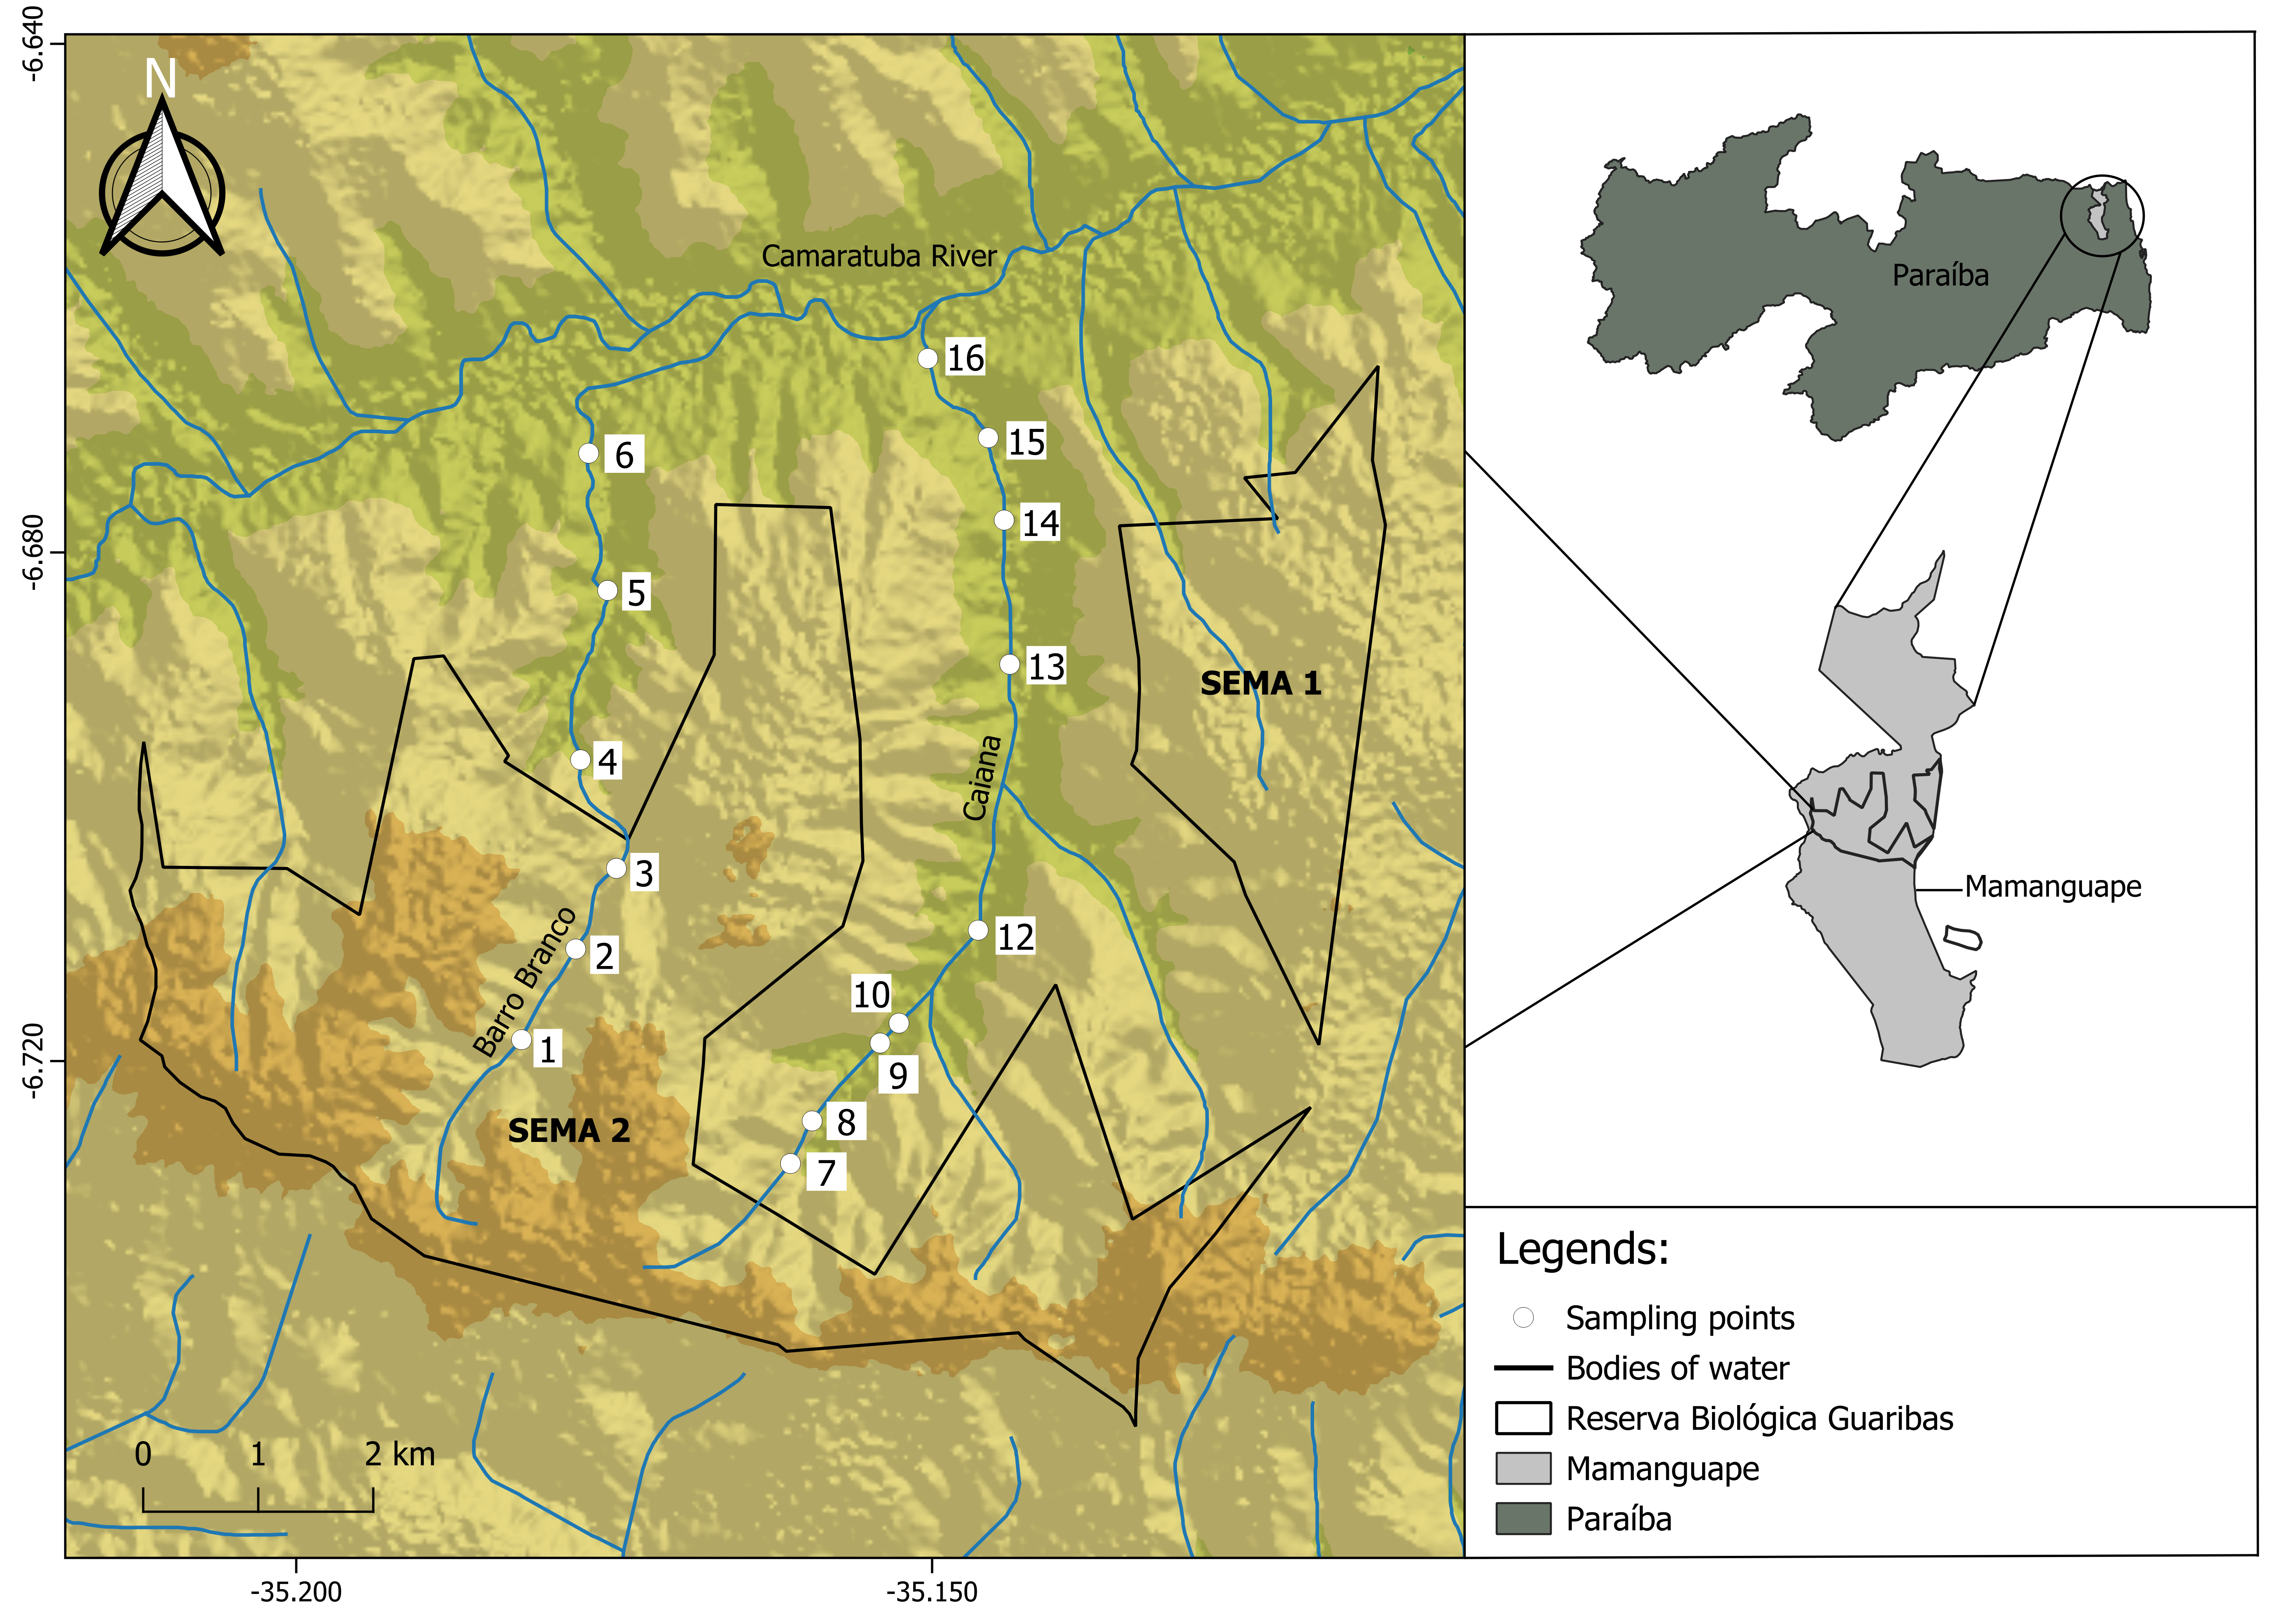
\includegraphics{imagens/Mapa.png}

}

\caption{\label{fig-mapa}Mapa da área de influência da REBIO Guaribas
localizada no município de Mamanguape.}

\end{figure}%

\begin{figure}

\centering{

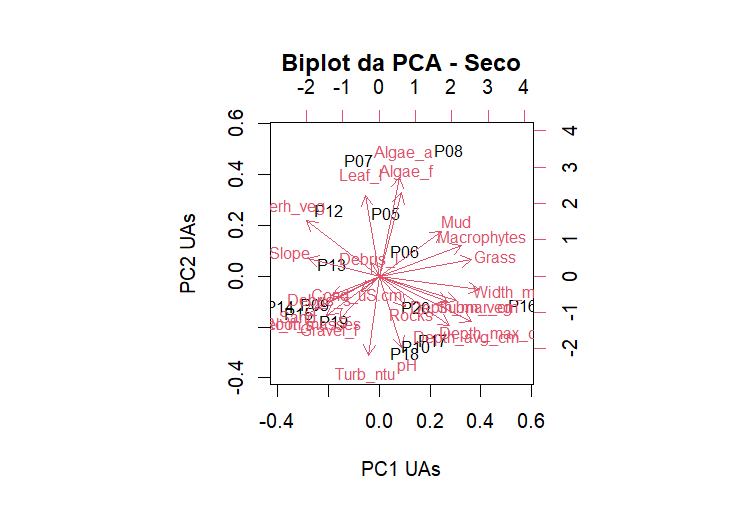
\includegraphics{imagens/PCA_Seco.png}

}

\caption{\label{fig-pcaseco}Biplot da Análise de Componentes Principais
(PCA) das unidades amostrais (UAs) e das variáveis ambientais nos
riachos Barro Branco e Caiana durante o período seco. Os pontos
representam as UAs, enquanto os vetores indicam as variáveis ambientais
associadas à estrutura do habitat.}

\end{figure}%

\begin{figure}

\centering{

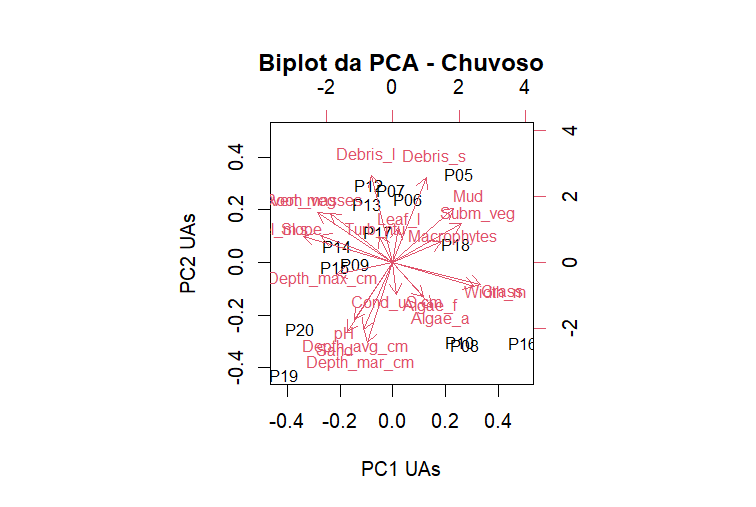
\includegraphics{imagens/PCA_Chuvoso.png}

}

\caption{\label{fig-pcachuvoso}Biplot da Análise de Componentes
Principais (PCA) das unidades amostrais (UAs) e das variáveis ambientais
nos riachos Barro Branco e Caiana durante o período chuvoso. Os pontos
representam as UAs, enquanto os vetores indicam as variáveis ambientais
associadas à estrutura do habitat.}

\end{figure}%

\begin{figure}

\centering{

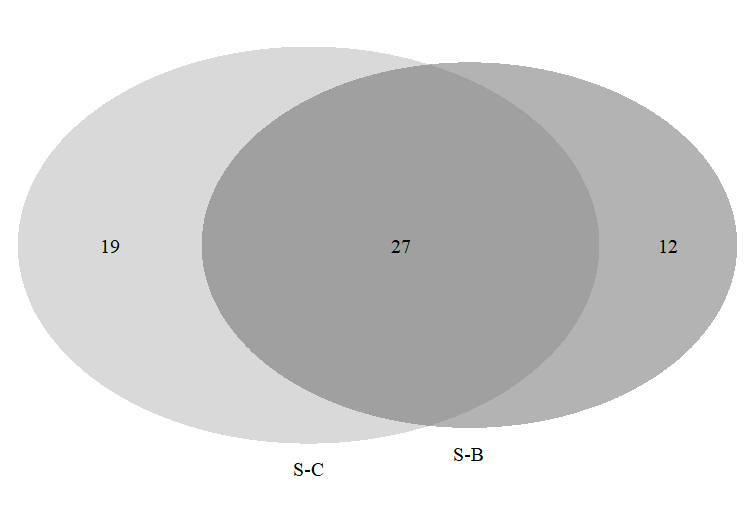
\includegraphics{imagens/venn_seco.png}

}

\caption{\label{fig-venn-seco}Diagrama de Venn indicando o número de
espécies compartilhadas e exclusivas representadas a partir dos
componentes de diversidade alfa (α) dos riachos Barro Branco (B) e
Caiana (C) da REBIO Guaribas no período seco (S).}

\end{figure}%

\begin{figure}

\centering{

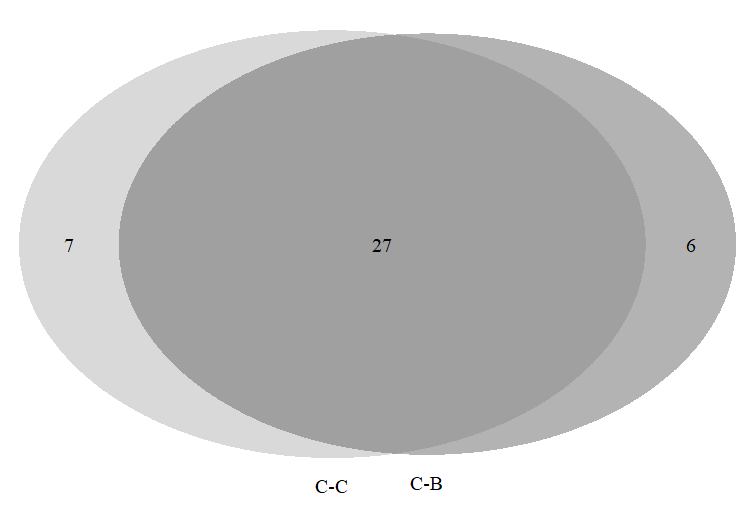
\includegraphics{imagens/venn_chuvoso.png}

}

\caption{\label{fig-venn-chuvoso}Diagrama de Venn indicando o número de
espécies compartilhadas e exclusivas representadas a partir dos
componentes de diversidade alfa (α) dos riachos Barro Branco (B) e
Caiana (C) da REBIO Guaribas no período chuvoso (C).}

\end{figure}%

\begin{figure}

\centering{

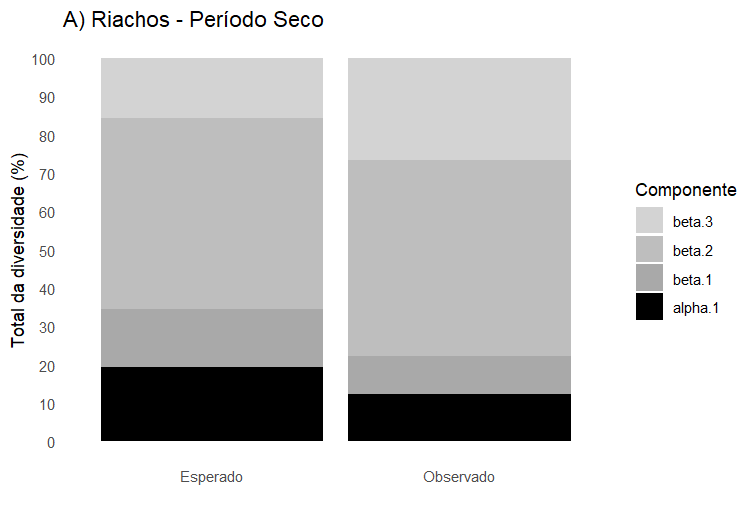
\includegraphics{imagens/diversidade_obs_seco.png}

}

\caption{\label{fig-diversidadeobs-riachos-seco}Diversidade observada e
esperada do período seco, dividida em componentes alfa e três/dois
betas, expressa em porcentagem da riqueza total em (A) ambos os riachos;
(B) Barro Branco; e (C) Caiana. Alpha.1 = unidade de amostragem, beta.2
= variação entre habitats; beta.2 = variação entre pontos; beta.3 =
variação entre riachos.}

\end{figure}%

\begin{figure}

\centering{

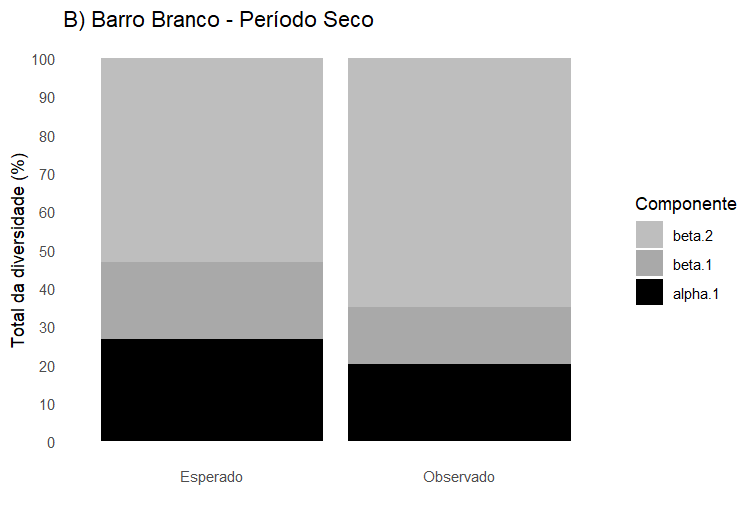
\includegraphics{imagens/diversidade_obs__bb_seco.png}

}

\caption{\label{fig-diversidadeobs-bb-seco}}

\end{figure}%

\begin{figure}

\centering{

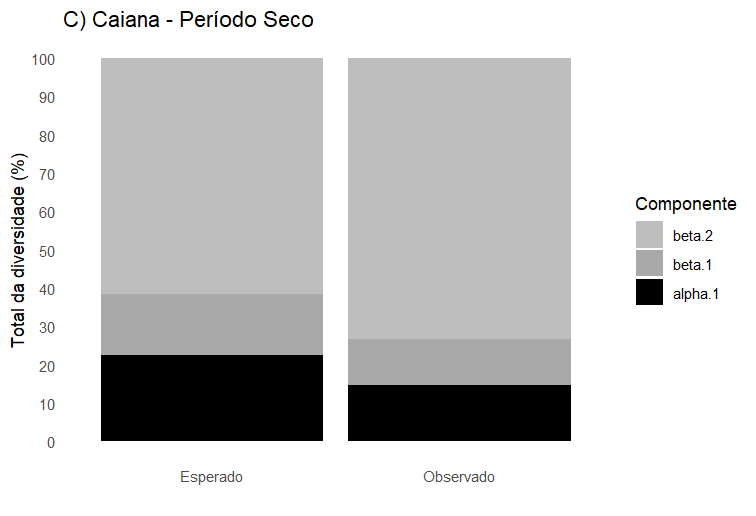
\includegraphics{imagens/diversidade_obs__ca_seco.png}

}

\caption{\label{fig-diversidadeobs-ca-seco}}

\end{figure}%

\begin{figure}

\centering{

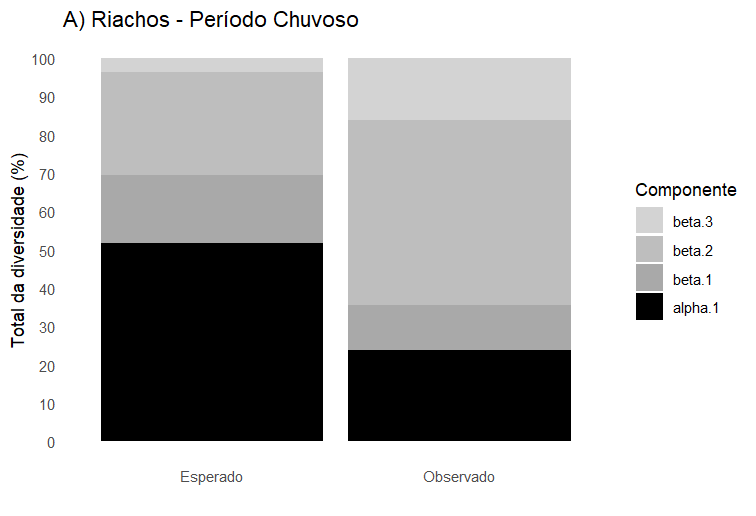
\includegraphics{imagens/diversidade_obs__chuvoso.png}

}

\caption{\label{fig-diversidadeobs-riachos-chuvoso}Diversidade observada
e esperada do período chuvoso, dividida em componentes alfa e três/dois
betas, expressa em porcentagem da riqueza total em (A) ambos os riachos;
(B) Barro Branco; e (C) Caiana. Alpha.1 = unidade de amostragem, beta.2
= variação entre habitats; beta.2 = variação entre pontos; beta.3 =
variação entre riachos.}

\end{figure}%

\begin{figure}

\centering{

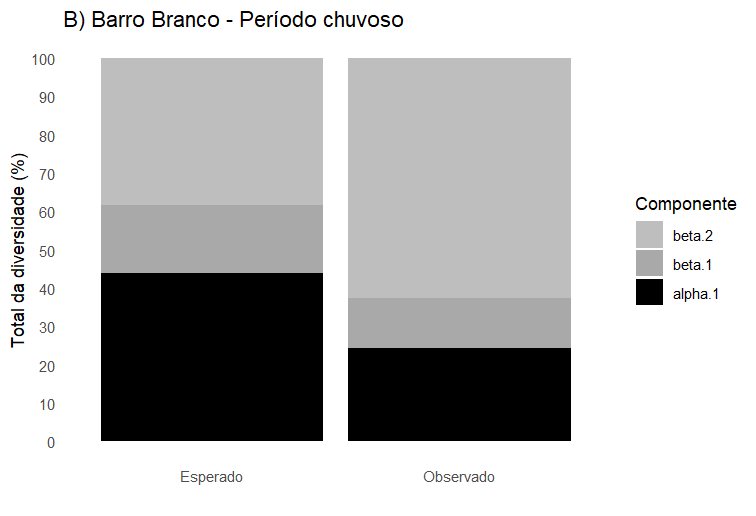
\includegraphics{imagens/diversidade_obs__bb_chuvoso.png}

}

\caption{\label{fig-diversidadeobs-bb-chuvoso}}

\end{figure}%

\begin{figure}

\centering{

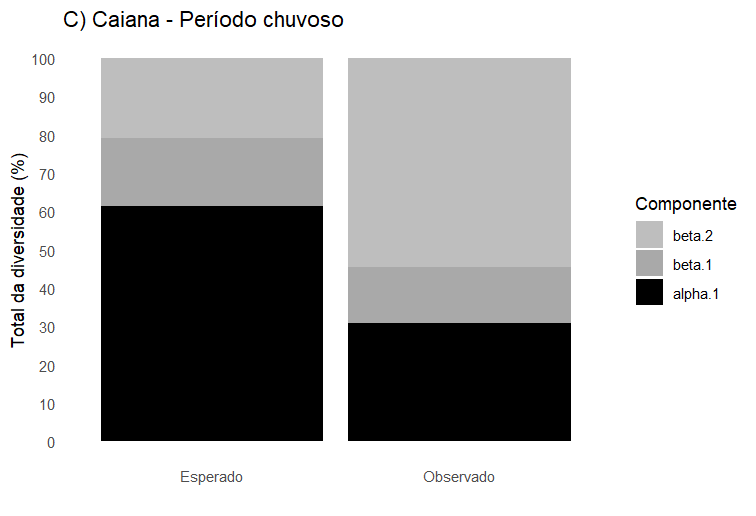
\includegraphics{imagens/diversidade_obs__ca_chuvoso.png}

}

\caption{\label{fig-diversidadeobs-ca-chuvoso}}

\end{figure}%

\begin{figure}

\centering{

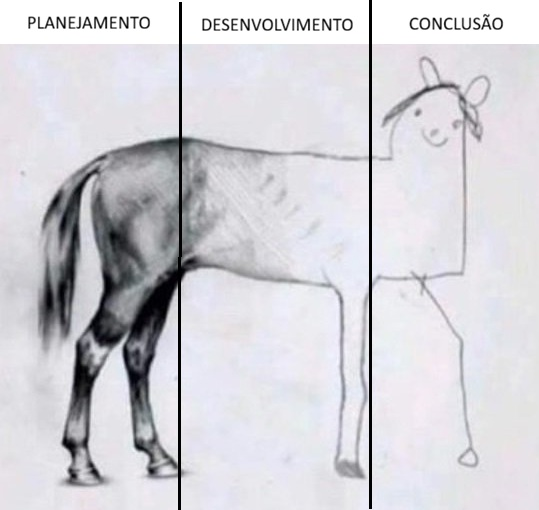
\includegraphics{imagens/pesquisa_cientifica.jpg}

}

\caption{\label{fig-pesquisa}Etapas do desenvolvimento da pesquisa
científica.}

\end{figure}%

\subsection*{Tables}\label{tables}
\addcontentsline{toc}{subsection}{Tables}

\pagebreak
\newpage

\section*{Apendices}\label{apendices}
\addcontentsline{toc}{section}{Apendices}

\section*{Non-used figures and
tables}\label{non-used-figures-and-tables}
\addcontentsline{toc}{section}{Non-used figures and tables}

\begin{tcolorbox}[enhanced jigsaw, colback=white, opacityback=0, titlerule=0mm, colbacktitle=quarto-callout-warning-color!10!white, arc=.35mm, leftrule=.75mm, bottomtitle=1mm, breakable, rightrule=.15mm, toptitle=1mm, colframe=quarto-callout-warning-color-frame, title=\textcolor{quarto-callout-warning-color}{\faExclamationTriangle}\hspace{0.5em}{Non-used codes}, toprule=.15mm, bottomrule=.15mm, left=2mm, opacitybacktitle=0.6, coltitle=black]

\end{tcolorbox}




\end{document}
